\documentclass[letterpaper, spanish, 12pt]{report}

%% PACKAGE SECTION
\usepackage{setspace}
\usepackage[letterpaper, margin=2.5cm]{geometry}
\usepackage[spanish]{babel}
\usepackage{graphicx}
\graphicspath{ {images/} }
\usepackage{booktabs}
\usepackage{multirow}
\usepackage{listings}
\usepackage{color}
\usepackage{amsmath}
\usepackage{float}
\usepackage[utf8]{inputenc}
\usepackage{titlesec}
\usepackage{lipsum}
%\usepackage{helvet}
\usepackage{caption}
\usepackage{booktabs}
\usepackage{adjustbox}
\usepackage{graphicx}
\usepackage{amsmath}
\usepackage{tabularx}
\usepackage[hyphens,spaces]{url}
\usepackage{listings} %For code in appendix

\definecolor{codegreen}{rgb}{0,0.6,0}
\definecolor{codegray}{rgb}{0.5,0.5,0.5}
\definecolor{codepurple}{rgb}{0.58,0,0.82}
\definecolor{backcolour}{rgb}{0.95,0.95,0.92}

\lstdefinestyle{mystyle}{
    backgroundcolor=\color{backcolour},
    commentstyle=\color{codegreen},
    keywordstyle=\color{magenta},
    numberstyle=\tiny\color{codegray},
    stringstyle=\color{codepurple},
    basicstyle=\footnotesize,
    breakatwhitespace=false,
    breaklines=true,
    captionpos=b,
    keepspaces=true,
    numbers=left,
    numbersep=5pt,
    showspaces=false,
    showstringspaces=false,
    showtabs=false,
    tabsize=2
}

\lstset{style=mystyle}

%% LANGUAGE SELECTION FOR SPANISH
\selectlanguage{spanish}

%% SET COUNTER CHAPTER
\setcounter{secnumdepth}{0}
\titleformat{\chapter}[display]{\normalfont\bfseries}{}{0pt}{\Huge}

%% FIX CAPTION STYLE FOR REFERENCES AND BIBLIOGRAPHY
\addto\captionsspanish{\renewcommand{\bibname}{Referencias}}
\renewcommand{\bibname}{Referencias}
\renewcommand{\familydefault}{\sfdefault}
\captionsetup{font=footnotesize}

%% SET FANCYHDR FOR PAGE NUMBERING
\usepackage{fancyhdr}
\fancyhf{} % clear all header and footers
\renewcommand{\headrulewidth}{0pt} % remove the header rule
\rhead{\thepage}
\pagestyle{fancy}
\pagestyle{myheadings}
\makeatletter
\def\@oddhead{{\slshape\rightmark}\hfil\footnotesize\thepage}%
\makeatother

%% CREATE MINARG AND MAXARG OPERATORS
\DeclareMathOperator*{\argmax}{argmax} % thin space, limits underneath in displays
\DeclareMathOperator*{\argmin}{argmin} % thin space, limits underneath in displays

%% R CODE LISTING
\lstset
{ %Formatting for code in appendix
    language=R,
    basicstyle=\footnotesize,
    numbers=left,
    stepnumber=1,
    showstringspaces=false,
    tabsize=1,
    breaklines=true,
    breakatwhitespace=false,
}

%% BEGIN DOCUMENT WITH ROMAN NUMBERING
\pagenumbering{roman}

\begin{document}
\begin{titlepage}
\begin{center}
\vspace*{1cm}    


\includegraphics[width=0.6 \textwidth]{logoubj.png} \\
\large{Universidad Benito Juárez G.}

\vspace{3cm}
\textbf{Ariel Estanislao Meilij Ezeiza}

\vspace{3cm}
\huge
Modelo Predictivo de la Tasa Representativa de Mercado de Colombia Utilizando Aprendizaje Automatizado

\vspace{3cm}
\large
\textbf{Tesis para obtener el grado de Doctor en Administración Gerencial}

\vspace{4cm}
\small
\textit{Julio 14 del 2018}

\end{center}
\end{titlepage}

\pagenumbering{gobble}

\Large
 \begin{center}
Resumen\\ 
\hspace{5pt}

% Author names and affiliations
\large
Ariel E. Meilij$^1,^2$  \\
\hspace{5pt}

\small  
$^1$) Universidad Benito Juárez G.\\
ariel.meilij@gmail.com\\
$^2$) Universidad Latinoamericana de Ciencia y Tecnología
\end{center}
\hspace{5pt}

\normalsize
El siguiente trabajo de investigación tiene como finalidad determinar un modelo de predicción para la tasa de cambio del dólar en Colombia (conocida legalmente como la TRM) utilizando aprendizaje automatizado. La investigación se enfoca en la hipótesis de que las series de tiempo pueden utilizarse como elementos de predicción por contener la tendencia de una variable, pero son más fuertes cuando se utilizan las variables exógenas que modelan e intervienen en dicho comportamiento. Para la TRM estas variables independientes son los regresores representados por los principales rubros de exportación del país. En vez de extraer un modelo en base a la observación, se utiliza el aprendizaje automatizado para entrenar los datos de las series de tiempo de la TRM y los rubros de exportación, y se unen con un modelo ensamblado de pronostico ARIMA para la serie de tiempo y regresión multivariable para los factores exógenos. 

\hspace{10pt}

\Large
 \begin{center}
Abstract\\ 
\hspace{5pt}
\end{center}

\normalsize
The following research thesis objective is the determination of a prediction model for the Colombian Peso exchange rate (legally known as the TRM) using machine learning techniques. The research focuses on the hipothesis that time series can be used for forecasting purposes given their intrinsic trend capacity, but their potential can be strengthened when coupled with exogenous variables that confound said behavior. For the TRM these independent variables are represented by the principal export components. Instead of extracting a model through observation, machine learning is used to train the different time series representing the values of the TRM and exports. Ensambled methodologies of stacking are then used to join the predictive capacities of ARIMA forecasting for TRM time series and multivariable regresion for the different export variables confounding the TRM pricing.
\clearpage
\begin{center}
    \thispagestyle{empty}
    \vspace*{\fill}
        Existen pocas metas en la vida profesional y académica de una persona como la investigación científica que implica el doctorado. Más allá de la dedicación personal, el esfuerzo de superación o la curiosidad humana que trata de abarcar un poco más de lo que se puede ver, entender o explicar, existe un cúmulo de personas que sacrifican su tiempo y aportan una cuota mayor de paciencia que el mismo doctorando. Todas estas personas fueron, son y serán el punto de apoyo para todos los empréstitos pasados, este en particular, y todos los proyectos futuros que puedan devenir. Por esa misma razón, estoy dedicando la siguiente tesis doctoral a las personas que la han hecho realidad.
            
        \begin{itemize}
            \item Primero que nada a mi esposa Ángela Alejo, quien ha sido la piedra angular de todo lo que soy y todo lo que seré en el futuro. 
            \item A nuestra hija Ruth Meilij, futura Física Cuántica, y una de las tantas (pocas) personas que entiende de \LaTeX y FORTRAN.
            \item A mis padres Norma Ezeiza y Ricardo Meilij, quienes siempre creyeron que lo lograría y sacrificaron muchos fines de semana para que pudiera estudiar.
            \item A mi jefe Max Harari por prestarme un libro de Big Data en el 2014 y despertar la curiosidad por la Ciencia de Datos. Siempre quise ser un Data Scientist, simplemente no sabía que existía tal cosa hasta que un libro me dejó más preguntas que respuestas. 
            \item A los profesores Roger Peng, Ph.D., Jeff Leek, Ph.D. y Brian Caffo, Ph.D. de \emph{Johns Hopkins University}. Gracias a sus clases y emprendimiento aprendí las habilidades de estadística, programación y matemáticas que me permitieron seguir investigando. 
            \item A los increíbles profesores de la Universidad Benito Juárez G. Es poco probable que entiendan la importancia y evolución que significan para todos los doctorandos del grupo G2V2. Por eso es tan importante que sepan que se está sembrando en estos momentos la nueva generación de investigadores del área de la Administración Gerencial en Latinoamérica gracias a sus esfuerzo. 
        \end{itemize}
    \vspace*{\fill}
    \end{center}
\clearpage

\tableofcontents
\listoffigures
\listoftables

%% CHANGE 1.5 SPACING ON STARTING HERE!
\begin{spacing}{1.0}
\begin{spacing}{1.5}
\pagenumbering{roman}
\setcounter{chapter}{-1}
\chapter{Introducción}
\thispagestyle{empty}

\section{Antecedentes de la Investigación}
Para todas las empresas que importan producto para su comercialización en el territorio de Colombia, el manejo de la TRM es uno de los problemas mayores que deben confrontar. La tasa de cambio representativa del mercado (TRM por sus siglas) es el valor en pesos colombianos que una empresa tiene que desembolsar por un dólar estadounidense. A pesar que no todas las importaciones provienen de Estados Unidos, inclusive aquellas que se realizan con Asia tienen facturación en dólares. De aquí que el dólar sea tan ubicuo en los procesos de comercio internacional, que Colombia como país importador y exportador haya tenido que crear una figura legal solamente para esta razón entre dos monedas. 

La TRM afecta una serie de variables dentro del proceso comercial de una empresa. 

\begin{itemize}
	\item Las listas de precios que emita el departamento de contabilidad estarán sujetas a la TRM en curso. Si el departamento de finanzas e importación no realizó la mejor negociación de la TRM, los precios se verán afectados de manera negativa, ya que su costo es mayor por afectación directa del cambio de dólares americanos a pesos colombianos.
	\item El departamento de ventas tendrá un especial interés en evitar las fluctuaciones constantes de listas de precio, que inevitablemente el departamento de contabilidad actualizará, si no puede prever la variación misma de la TRM en un horizonte de corto a mediano plazo. 
	\item Asimismo, el departamento de mercadeo vigilará de cerca que la variación de precios sea mínima, ya que la variable precio es una de las 4 P’s de la ciencia de la mercadotecnia (siendo todas posicionamiento, precio, producto y publicidad). La variación del precio al alza aliena a los consumidores, que pueden no ver la razón de la misma en el aumento de la TRM sino en la mala fe del importador. 	
\end{itemize}

Para protegerse de los efectos de la variación de la moneda, las empresas algunas veces recurren al concepto de forwards, o contratos de compras a futuros de moneda extranjera pactados a un precio dado que reduce el margen de incertidumbre. Dentro de la contabilidad moderna, y aplicado a la importación de productos, el contrato de forward es un elemento de costeo. Con esto la empresa puede asignar costos a un producto a un valor dado de tasa de cambio el cual es conocido y no sufrirá variación. Esto no implica que sea el mejor valor o el mejor negociado, solo que el precio final al momento de ejecutarse el contrato no sufre variación y no hay incertidumbre sobre el mismo. 

Muchas empresas no efectúan contratos de compra de moneda a futuro haciendo acuso del carácter especulativo de los mismos. El horizonte de planificación de un importador involucra un ciclo de noventa a ciento veinte días en el cual factura y cobra sus ventas a crédito. Dentro de ese plazo, es probable que la TRM haya reducido por debajo del valor pactado en el contrato futuros, incurriendo en gastos innecesarios por reducir la incertidumbre del cambio. Otras empresas solo cubren una porción del valor total de la operación con contratos futuros tratando de optimizar el resultado de la misma y perder el menor margen posible de rentabilidad versus el costo de cobertura. 

El problema mayor para todas estas empresas es poder predecir con algún valor matemático y científico cuál será el valor de la TRM en cualquier momento dado. Existe en la comunidad financiera - y en la comunidad de comerciantes en general - una idea acertada de que la TRM está relacionada a los movimientos del precio internacional del petróleo, principal producto de exportación de Colombia, y por ende, el mayor contribuyente a estabilizar la balanza de pago del país y la necesidad de equilibrar los flujos de moneda internacional con las reservas nacionales. Estos estudios incluyen los reportes de casas financieras importantes como J. P. Morgan, las cuales han analizado las fluctuaciones de la cesta petrolera y la TRM hasta un índice de correlación cercano al 70 por ciento (o en términos matemáticos, un coeficiente de correlación \(R^{2} ~ 0.7\) ). 

Para el estadista entrenado, un índice de correlación \(R^{2}\) de 0.7 en un buen indicio de correlación, pero lejos de un valor que pueda completar un modelo de predicción. Para la ciencia de datos, es sin embargo un comienzo prometedor de un modelo predictivo en potencia que puede construirse a través de las nuevas metodologías de Aprendizaje Automatizado. El aprendizaje automatizado utiliza técnicas matemáticas y de estadística avanzadas para aprender de los datos históricos y crear modelos de predicción altamente confiables. El aprendizaje automatizado no es inteligencia artificial (aunque la inteligencia artificial usa aprendizaje automatizado), sino que es el conjunto de herramientas de la ciencia de datos que hoy ayuda a diseñar teclados que predicen el texto, motores de búsqueda en Internet, autos que se manejan solos, y búsqueda de solución a enfermedades como el cáncer. 

¿Hay una manera más eficaz de poder modelar y predecir la TRM para minimizar los efectos negativos de las variaciones de la misma en la comercialización de productos importados? ¿Hay otros elementos además de la cesta de petróleo que jueguen un papel determinante en la fijación del valor de la TRM? ¿Si la Superintendencia sólo mide el valor en base al intercambio de compradores y vendedores, como juegan estos dos en la fijación del precio si son solo agentes secundarios de procesos de importación y exportación?

Una empresa que cuente con el conocimiento y tecnología para poder predecir y proyectar el valor de la TRM podrás reducir el impacto negativo en el proceso de comercialización mientras que optimiza el rendimiento financiero en sus áreas contables. 

\section{Objetivo general}
El objetivo principal de la investigación es construir un modelo parsimonioso predictivo que permita determinar el valor futuro de la TRM a partir de variables predictivas dadas.

\subsection{Objetivos específicos}
Los objetivos específicos de la investigación son los siguientes:

\begin{itemize}
	\item Identificar que variables dentro del marco económico colombiano son las que tienen mayor grado de incidencia en la determinación de la TRM colombiana. 
	\item Cuantificar cuales y cuantas de estas variables forman parte de un modelo predictivo parsimonioso que permita realizar predicciones dentro de un intervalo de confidencia con valores de p = 0.05. 
	\item Determinar qué tipo de modelo parsimonioso es el correcto utilizando las variables predictivas del punto anterior con los mismos intervalos de confidencia, o en su defecto si este es un modelo predictivo compuesto. 
\end{itemize}

\section{Justificación de la investigación}
La justificación de dicha investigación está basada en el costo que afrontan las empresas que no pueden determinar exactamente el valor de la TRM dentro de su ciclo operativo anual e incurren en pérdidas dadas por:

\begin{enumerate}
	\item Falta de ventas al costear incorrectamente sus productos por encima del valor de mercado
	\item Perdidas contables al costear incorrectamente sus productos a valor del mercado y luego verificar que no están cubiertas las deudas en moneda extranjera y que la TRM tiene un valor superior al utilizado
	\item Perdidas contables en los contratos futuros de compra de divisas con los bancos en el cual el precio de ejecución termina siendo superior al valor actual de la TRM (en dicho caso, para el banco es una operación altamente rentable)
\end{enumerate}

Adicionalmente, la siguiente investigación plantea el uso de una metodología relativamente nueva en el campo de la administración como lo es el aprendizaje automatizado. La ciencia de datos es una disciplina principalmente multidisciplinaria, que recién ahora comienza a tener alguna participación oficial en algunas universidades del mundo. El enfoque ha sido utilizado con éxito en la ingeniera y ciencias de la computación, así como en la bioestadística, pero es muy poco su uso académico en las ciencias administrativas y financieras, por lo que el enfoque es novedoso y abre las puertas a la resolución de muchos más problemas con una metodología cuantitativa similar.

\section{Alcances y Limitaciones}
Las siguientes son los alcances y limitaciones de la investigación. 

\begin{itemize}
	\item El siguiente estudio está basado en la TRM colombiana, que por su propia definición establece una razón entre dos divisas, el peso colombiano y el dólar estadounidense. Aun cuando la solución prevista al problema muy probablemente pudiera utilizarse con otras monedas, esta investigación no las abarca.
	\item El siguiente estudio no hace referencia ni analiza en profundidad el sistema para determinar la TRM por parte de la Superintendencia Financiera de Colombia; este pudiera ser un tema interesante de tesis de posgrado para un futuro investigador. El resultado final del método de la Superintendencia Financiera de Colombia para el valor de la TRM se utiliza solo como una observación matemática de un hecho predecible a partir de ene cantidad de variables. 
	\item El siguiente estudio utiliza base de datos y datos oficiales históricos medidos desde el año 2000 hasta el año 2017. Si bien este valor es menor al de una generación, ha sido arbitrariamente establecido como punto de quiebre ya que reúne muchos más datos estadísticos de los necesarios para un modelo predictivo de gran precisión. 
	\item La siguiente investigación busca un modelo predictivo parsimonioso. Un modelo parsimonioso en estadística es un modelo que cumple con el valor predictivo buscado con el menor número de variables predictivas necesarias. Puede entonces existir variables predictivas que afecten el valor de la TRM pero que este estudio no incluirá si el resultado del modelo predictivo es suficiente con un número menor de variables.
\end{itemize} 
\end{spacing}
\pagenumbering{arabic}
\setcounter{chapter}{0}
\chapter{Capítulo I: \\Protocolo de Investigación}
\thispagestyle{empty}

\section{El Problema de Investigación}
El siguiente proyecto de investigación busca analizar el problema de la determinación del valor futuro de la TRM de Colombia en base a los componentes principales de exportación del país, que conforman su cesta de divisas, con miras a crear un modelo predictivo matemático que le sirva a la organización para la optimizar los procesos comerciales y financieros de la misma. ¿Qué es la TRM que afecta tanto el funcionamiento de los importadores? Actualmente la Superintendencia Financiera de Colombia es la que calcula y certifica diariamente la TRM con base en las operaciones registradas el día hábil inmediatamente anterior y la define de la siguiente manera (Circular Reglamentaria Externa del Banco de la República DODM-146, 2015):

\begin{quotation}
	La tasa de cambio representativa del mercado (TRM) es la cantidad de pesos colombianos por un dólar de los Estados Unidos (antes del 27 de noviembre de 1991 la tasa de cambio del mercado colombiano estaba dada por el valor de un certificado de cambio). La TRM se calcula con base en las operaciones de compra y venta de divisas entre intermediarios financieros que tranzan en el mercado cambiario colombiano, con cumplimiento el mismo día cuando se realiza la negociación de las divisas.
\end{quotation}

La Superintendencia Financiera de Colombia no determina el valor de la TRM sino de un elemento derivado de las operaciones de compra y venta de la misma. Son los agentes de operación (exportadores que venden sus productos en dólares y los deben canjear a pesos colombianos e importadores que compran sus productos en dólares y para tal fin cambian sus pesos colombianos). Ambos obedecen a fuerzas del mercado que dan forma y materializan la valorización. 

Es de conocimiento que la cesta petrolera influye en la valorización de la TRM, sin embargo, poco o nada se ha estudiado de que otras variables actúan en la ecuación total. Cada una de estas debe pensarse como una variable independiente de un modelo predictivo que interviene en la valorización total de la TRM, y sin los cuales la formula queda incompleta.

\section{Impacto Social}
El trabajo cumple con la dimensión de relevancia social. Ninguna empresa quiere costear sus productos por encima de los demás agentes del mercado, so pena de perder participación de mercado a sus competidores con precios más ventajosos. La capacidad de estimar a futuro el mejor pronóstico de tasa de cambio reduce el porcentaje de carga por previsión de volatilidad de moneda (también conocido en contabilidad como colchón) lo que redunda en un precio mejor para el consumidor y la sociedad en general. Al reducir las ineficiencias del cálculo de costos prediciendo de forma correcta la tasa de cambio los consumidores ganan el diferencial entre el precio pobremente estimado y un precio ajustado a las realidades del cambio futuro.

\section{Línea de Investigación}
El siguiente trabajo de investigación se apega a la línea de investigación financiera de la UBJ. La universidad define la línea financiera como aquella que investiga modelos económicos y financieros innovadores que impulsen el crecimiento y sustentabilidad de la organización a fin de relevar su competitividad \cite{guiaAcademicaDAG}. 

La hipótesis de trabajo de la investigación propone un nuevo modelo de predicción de la tasa de cambio de Colombia utilizando aprendizaje automatizado y un modelo ensamblado de aprendices, lo que representa un enfoque innovador para mejorar la situación de optimización de costos y competitividad de la empresa. 

\section{Tipo de Estudio}
El tipo de estudio es hipotético deductivo, cuantitativo.

Es hipotético deductivo porque:

\begin{itemize}
\item Partimos de una teoría base (macroeconomía que sustenta la tasa de cambio con la balanza de pagos y exportaciones, machine learning para deducir modelos predictivos en base a grandes muestras de datos) 
\item Formulamos una hipótesis de trabajo
\item Aplicamos ciencia de datos para una recolección masiva de datos de diferentes regresores (cada uno un rubro importante de exportaciones de Colombia)
\item Confirmamos la hipótesis al extraer un modelo predictivo estadístico  
\end{itemize}

\section{Pregunta de Investigación}
La pregunta de investigación de este anteproyecto surge de una pregunta real y de aplicación necesaria en el ámbito empresarial de una organización importadora de bienes de consumo masivo al mercado de Colombia: \emph{¿Cómo podemos predecir la TRM para mitigar el efecto negativo de las fluctuaciones en la tasa de cambio en la contabilidad de precios y costos?}

\section{Objetivo General de la Investigación}
El objetivo principal de la investigación es construir un modelo parsimonioso predictivo que permita determinar el valor futuro de la TRM a partir de variables predictivas dadas.

\subsection{Objetivos específicos}
Los objetivos específicos de la investigación son los siguientes:

\begin{itemize}
	\item Identificar que variables dentro del marco económico colombiano son las que tienen mayor grado de incidencia en la determinación de la TRM colombiana. 
	\item Cuantificar cuales y cuantas de estas variables forman parte de un modelo predictivo parsimonioso que permita realizar predicciones dentro de un intervalo de confidencia con valores de p = 0.05. 
	\item Determinar qué tipo de modelo parsimonioso es el correcto utilizando las variables predictivas del punto anterior con los mismos intervalos de confidencia, o en su defecto si este es un modelo predictivo compuesto. 
\end{itemize}

La intención del trabajo de investigación es integrar el uso de rubros de exportación como series de tiempo para el entrenamiento de modelos de aprendizaje automatizado en forma de aprendices. La determinación del modelo no la hace el investigador sino que la metodología de aprendizaje automatizado ayuda a entrenar los datos para extraer el modelo. Uno o ambos de estos modelos debe cumplir con la premisa de alcanzar un alto nivel de predicción. Si ambos modelos cumplen con la premisa de alto valor predictivo entonces sus egresos - los valores estimados - serán utilizados como entradas de un tercer modelo ensamblado (conocido en inglés como modelo apilado o \textit{stacking}) para diseñar un modelo predictivo parsimonioso final con mayor valor de precisión.   

\section{Alcances y Limitaciones}
Las siguientes son los alcances y limitaciones de la investigación. 

\begin{itemize}
	\item El siguiente estudio está basado en la TRM colombiana, que por su propia definición establece una razón entre dos divisas, el peso colombiano y el dólar estadounidense. Aun cuando la solución prevista al problema muy probablemente pudiera utilizarse con otras monedas, esta investigación no las abarca.
	\item El siguiente estudio no hace referencia ni analiza en profundidad el sistema para determinar la TRM por parte de la Superintendencia Financiera de Colombia; este pudiera ser un tema interesante de tesis de posgrado para un futuro investigador. El resultado final del método de la Superintendencia Financiera de Colombia para el valor de la TRM se utiliza solo como una observación matemática de un hecho predecible a partir de ene cantidad de variables. 
	\item El siguiente estudio utiliza base de datos y datos oficiales históricos medidos desde el año 2000 hasta el año 2017. Si bien este valor es menor al de una generación, ha sido arbitrariamente establecido como punto de quiebre ya que reúne muchos más datos estadísticos de los necesarios para un modelo predictivo de gran precisión. 
	\item La siguiente investigación busca un modelo predictivo parsimonioso. Un modelo parsimonioso en estadística es un modelo que cumple con el valor predictivo buscado con el menor número de variables predictivas necesarias. Puede entonces existir variables predictivas que afecten el valor de la TRM pero que este estudio no incluirá si el resultado del modelo predictivo es suficiente con un número menor de variables.
\end{itemize} 

\setcounter{chapter}{1}
\chapter{Capítulo II: \\Fundamento Teórico}
\thispagestyle{empty}

\section{Estado del Arte}
A pesar de ser un campo relativamente nuevo, la Ciencia de Datos está profundamente sustentada por la teoría académica (quizás por sus implicaciones como campo multidisciplinario y su importancia para la solución de problemas que impactan otras disciplinas).

De acuerdo a la bibliografía existente, la primera persona en hacer un bosquejo de la idea fue el académico Danés Peter Naur en su libro “Concise Survery of Computer Methods”. Naur sin embargo utiliza el término más que nada para sustituir el de ciencia computacional \cite{naur}. El investigador de Laboratorios Bell y profesor de la Universidad de Princeton, John Tukey, hace un mejor acercamiento al escribir el primer artículo científico sobre como la disciplina de la estadística cambiaba con el advenimiento de la informática \cite{tukey}. Mucho más tarde fue el estadista de la Universidad de Tokio Chikio Hayashi quien definiría de manera sucinta el concepto de Ciencia de Datos como un concepto sintético para unificar la estadística, el análisis de datos y los métodos relacionados con la consecución lo resultados \cite{hayashi}.

Es interesante que los métodos de aprendizaje automatizado proliferaron de forma paralela al concepto de ciencia de datos, y solo fueron absorbidos por esta en los últimos diez años. Alpaydim nos describe el aprendizaje automatizado como la programación de computadoras para optimizar un criterio de desempeño utilizando datos o experiencia pasada \cite{alpaydin}. Tom Mitchell respeta este concepto al describir el aprendizaje automatizado como “… la construcción de programas computacionales que aprenden con la experiencia…” \cite[pag. XV]{mitchell}. Solo Peter Harrington utiliza una descripción mucho más simplista al determinar que “El aprendizaje automatizado es la extracción de información de la data.” \cite[pag. 5]{harrington}.

La teoría detrás de la regresión lineal es bastante homogénea a través de todos los autores. Zumel y Mount describen la regresión lineal como el más común de los métodos de aprendizaje automatizado \cite{zumelMount}, y si no, es muy fácil verificar cual otro método probar como segunda opción. Para Daroczi, el énfasis está en los modelos de regresión multivariable (una extensión de la regresión lineal simple de un solo predictor y resultado) que construyen el camino para la predicción de fenómenos complejos en la naturaleza y negocios \cite{daroczi}. Por su parte, Harrington resume los beneficios de la regresión lineal \cite{harrington} por la facilidad de interpretar los resultados y lo frugal en el uso de ciclos de computación (aunque puede ser menos útil si el fenómeno no es perfectamente lineal).
 
Muchos autores han escrito sobre las series de tiempo, pero es difícil agregar al tema o discutir las ideas del profesor Robert Hyndman, uno de los expertos más respetados en la comunidad de la estadística por su trabajo en las series de tiempo. Hyndman extiende la teoría a las series de tiempo como elementos de pronóstico y su relación con la regresión lineal \cite{hyndman}. Desde el punto de vista técnico, Hyndman es el creador de varias bibliotecas de funciones de pronóstico utilizando series de tiempo y ARIMA en lenguaje R. Dentro de la bibliografía, Daroczi es quien agrega detalles sobre la detección temprana de valores atípicos que pueden dificultar – y mucho – el análisis \cite{daroczi}. Un componente importante de las series de datos es la detección de si son o no auto-regresivas (lo que determina mucho de su poder predictivo). La fórmula para la detección de series auto-regresivas es el test Dickey-Fuller, y la mejor bibliografía es el artículo científico escrito por ambos profesores en la revista especializada Econometrica \cite{dickeyfuller}. A pesar de ser un artículo contemporáneo, la teoría detrás de la prueba Dickey-Fuller nos permite descartar series de tiempo no-regresivas con poco poder de predicción.
 
El uso de modelos ensamblados es en cierta forma la prueba final de la hipótesis de trabajo: la utilización de dos modelos entrecruzados cuyos resultados conforman una tabla temporal de valores esperados de los cuales se genera un nuevo modelo sintético de predicción más general y con mayor capacidad de predicción en juegos de datos de validación cruzada. Este concepto es novel; Witten y Frank lo describen como combinación de métodos múltiples, y escriben: “… un enfoque obvio para hacer mejores decisiones es tomar el resultado de diferentes métodos y combinarlos…” \cite{datamining}. Zhou nos describe que “… los modelos ensamblados que entrenan múltiples variables y luego las combinan para uso de entrenamiento, con el Boosting y el Bagging como representantes principales, representan lo más novedoso en el estado del arte de la ciencia de datos…” \cite[pag. 5]{ensembleMethods}. De una manera un tanto más coloquial, Zhang y Ma describen el uso de modelos ensamblados con una analogía de la vida real, en la cual los pacientes buscan una segunda y hasta tercera opinión de expertos antes de someterse a una operación complicada \cite{ensembleMachineLearning}. Curiosamente tanto Zhang, Ma y Zhou hablan de la combinación de métodos de regresión general con clasificadores, y solo Witten y Frank hablan de otras combinaciones (por supuesto, Witten y Frank comenzaban a escribir en los albores del ensamblaje de métodos, cuando los clasificadores no estaban tan de moda porque el análisis era mayoritariamente de números, algo que cambió con el avance de las redes sociales).

En su libro “Crisis Cambiarias en Países Emergentes” el Dr. Bernardo Carriello utiliza un modelo de descripción (más que de predicción) de corrida de las tasas de cambios, en el cual los regresores incluían variables de medición económicos como crédito privado como porcentaje del PIB, tasa de variación de reservas, desalineación de tipo real, y otros \cite{crisisCambiarias}. Carriello utiliza muchísimo modelos lineales dicotómicos que modelan los escenarios con variables binarias (algo muy común entre los economistas) que por lo general favorecen regresiones logísticas o con la utilización de variables dummy o comodín (se multiplican por el coeficiente uno o cero según tengan o no valor). La mayoría de la bibliografía de aprendizaje automatizado y ciencias de datos prefieren el estudio de variables continuas y reales con amplitud de rango y valores, algo que está más cerca de la disciplina de la bioestadística que de la economía. Una pregunta adicional válida es si tomar metodologías más cercanas a la bioestadística se aplica para la predicción financiera mejor que los modelos dicotómicos actuales.
 
Volviendo a la pregunta mayor de área, el autor y antiguo Ministro de Economía de Colombia, Alfonso Ortega Cárdenas, menciona como material de bibliografía universitaria, la re-valorización del dólar frente al peso colombiano tras el comienzo de la caída de los precios del petróleo a partir del año 2015 \cite{cardenas}. El Dr. Cárdenas no hace mucho hincapié en la correlación de ambas variables, y prefiere ahondar en temas macro-económicos como la variación de la tasa de interés como elemento de presión en la tasa cambiaria y las leyes de ingreso de capital extranjero. Pero es claro que el efecto de las fuentes de ingreso del petróleo como variable clave en el valor final de la TRM ya han sido definidas – si bien algo ligeramente – como claves en un libro de texto de economía de Colombia. ¿Hay elementos adicionales que indiquen la importancia de otras fuentes de ingresos como posibles modeladores y variables de predicción de la TRM? Si los hay, y aparecen en la misma bibliografía de Cárdenas quien describe en detalle a) el sector petrolero, b) el sector siderúrgico, c) el carbón, y d) el níquel.

Los autores Castaño, Callejas, Ochoa y Henao de la Facultad de Ciencias Económicas de la Universidad de Antioquia, hacen un trabajo innovador y de avanzada técnicas estadísticas en su artículo científico \emph{Modelando el Esquema de Intervenciones del Tipo de Cambio para Colombia}. En dicho escrito se determina la eficiencia de las intervenciones realizadas por el Banco de la República empleando el modelo teórico del canal de coordinación. Los autores evalúan el efecto que tiene el diferencial de tasas de interés, la variable de intervenciones construida por medio de un modelo \emph{Markov-switching}, y el procedimiento de inversionistas técnicos y fundamentalistas sobre diferentes cuantiles del retorno de la tasa representativa del mercado (TRM). La metodología utilizada son las regresiones de cuantiles bajo redes neuronales \cite{modelandoIntervenciones}. Castaño, Callejas, Ochoa y Henao no son los únicos en utilizar redes neuronales, o una variante de redes neuronales, para entrenar modelos de predicción. Los profesores de la Universidad de Parana, Brasil, Scarpin y Steiner utilizan un modelo de Redes Neuronales Radiales Artificiales para un modelo de pronóstico de reemplazo de artículos vendidos en supermercados \cite{scarpinSteiner}. Sin embargo el modelo propuesto por Scarpin y Steiner necesita alimentarse no solo de la data actualizada de movimientos de producto, sino de un pronóstico inicial de necesidades de niveles de venta. Con una base similar - la necesidad de un pronóstico a priori - pero una metodología diferente, los doctores Wang y Xu crean un marco para pronosticos cooperativos utilizando modelos basados en Pronósticos Combinados de Bayes \cite{wangXu}. 
 
Los investigadores Mehreen Rehman, Gul Muhammad Khan y Sahibzada Ali Mahmud han utilizado la ciencia de datos para la predicción de FOREX. Los autores utilizan CGP (Programación Genética Cartesiana), una extensión del uso de redes neuronales, para obtener predicciones del dólar australiano con 98.72\% de precisión por períodos extendidos de hasta 1,000 días \cite{rehmanKhanMahmud}. Los autores alimentan el sistema CGP con información histórica de las monedas en cuestión compuesta por 500 días de cotización.
 
Quizás menos conocido es el uso de clasificadores versus regresores. Este camino toma el estudio de los doctores Hossein Talebi, Winsor Hoang y Marina Gavrilova. En su investigación en búsqueda de la mejora de sistemas automatizados de corretaje de FOREX utilizando aprendizaje automatizado, los autores proponen un nuevo método de clasificación. Dicho método utiliza extracción de clasificadores de múltiples escalas para el entrenamiento de datos, y luego se ensamblan diferentes clasificadores por voto Bayes \cite{talebiHoang}. El método propuesto demuestra superioridad a la hora de ensamblar clasificadores por encima de clasificadores individuales.
 
Otro estudio interesante es el de los profesores de matemática de la universidad de Beijing Lean Yu, Shouyang Wang, y K. K. Lai. El enfoque es novedoso en el sentido que utilizan un sistema ensamblado de auto-regresión lineal generalizada (GLAR) con redes neuronales artificiales (ANN). Los autores llegan a la conclusión que los resultados en las predicciones son superiores a los resultados de las predicciones de los métodos por separado, o de métodos similares con regresiones lineales \cite{yuWangLai}. Una lectura cuidadosa de los resultados evidencia márgenes de error del 1.56\% al 3.57\%, dependiendo de la moneda a evaluar.

\section{Marco Teórico}
La Ciencia de Datos se caracteriza por ser una ciencia multidisciplinaria. A la par de extenso conocimiento de estadística y programación, el científico de datos debe poseer un dominio extremo sobre el campo de acción o \textit{domain expertise} como se le conoce en inglés \cite{pengMatsui}. Este portafolio de conocimiento se refleja de igual manera en el marco teórico del trabajo de investigación, que debe unir, analizar y sintetizar la teoría de la estadística descriptiva e inferencial, el aprendizaje automatizado y los modelos ensamblados para la resolución del problema, y la economía de Colombia para entender el problema en toda su magnitud. Por tales razones se ha decidido desglosar el marco teórico en seis secciones diferentes, cada una con su base de conocimiento distintivo. 

\begin{enumerate}
    \item La Economía de Colombia
    \item Regresión Lineal
    \item Series de Tiempo
    \item La Ciencia de Datos
    \item Aprendizaje Automatizado
    \item Modelos Ensamblados
\end{enumerate}

Cada una de estas secciones se unen en un todo final para una solución holística del problema de investigación.

\section{Economía de Colombia}
Para la creación de un modelo de predicción de la TRM de Colombia, tomando como hipótesis de trabajo que existe un número finito y reducido de variables de aporte que regulan el valor de la misma a través de los ingresos por exportación y su contribución a la economía nacional, se debe primeramente comprender y definir estos conceptos. La sección del marco teórico que cubre la economía de Colombia, tiene como finalidad abarcar los siguientes temas. 

\begin{enumerate}
	\item Definir correctamente el concepto de tasa de cambio y su específico colombiano, la tasa de mercado representativa, desentrañando la formula que usa la Superintendencia Bancaria para su valuación diaria.
	\item Entender las bases del comercio internacional de Colombia y cuales son sus principales productos de exportación, sobre todo con el afán de identificar correctamente candidatos como variables de aporte para alimentar de datos el modelo de aprendizaje automatizado. 
	\item Por último, especificar el funcionamiento de los elementos financieros derivados de compra de divisas tales como los \emph{forward} y su correspondiente reglamentación bajo la leyes de Colombia. 
\end{enumerate}

Entender el funcionamiento de la economía de Colombia, sus principales componentes de exportación, y los marcos legales que rigen las estructuras de la TRM y los productos financieros de compra y venta de divisas, nos da luces no solo para entender correctamente el problema, sino para plantear propuestas de solución matemáticas que tengan una amplia correlación entre el modelo abstracto y el comportamiento en la vida real del proceso. 

\subsection{La Tasa de Cambio}
La moneda de un país tiene una equivalencia en moneda de otro y ese valor se conoce como tasa de cambio. Explicamos el concepto apoyados en los escritos del autor Mauricio Cárdenas \cite{cardenas}. También es importante explicar porqué los productos de exportación tienen un efecto en la canasta de divisas y la balanza de pagos \cite{crisisCambiarias}.   

\subsection{La TRM}
Dennis Robertson \cite{robertson} definió el dinero como \textit{"todo aquello generalmente aceptado para el pago de una obligación"}. El dinero en su forma más simple es el medio de pago de total liquidez, constituido por el \textit{efectivo} (billetes y monedas) y puesto en circulación por la Banca Central y por el \textit{dinero bancario}, correspondiente a los depósitos en bancos comerciales que son transferibles por medio de cheque. 

El intercambio de bienes y comercio internacional se realiza tomando como premisa que países con diferente moneda tendrán que llegar a algún tipo de mecanismo para compensar las compras, ventas y pagos de las mismas entre ambos actores. A falta de una moneda común (por lo menos en términos legales) el mecanismo que rige dicha condición de medio de operación es la tasa de cambio.

\subsubsection{Concepto: Tasa de Cambio}
Para entender el concepto de la tasa representativa de mercado, es importante primero entender el concepto de tasa de cambio. Dicha idea es muy sencilla, y gira entorno al valor de una moneda en relación con otra \cite{30seconds}. En épocas pasadas, el tipo de cambio era fijo, pero esta teoría ha quedado atrás con la implementación de tipos de cambio de flotación libre. La preocupación de los gobiernos gira en procurar mantener un determinado tipo de cambio ni estimule la revalorización de la moneda, ni mucho menos genere una devaluación de la misma \cite{cardenas}. 

\subsubsection{Devaluación de la Moneda} 
Se entiende como devaluación monetaria la pérdida del valor nominal de la moneda nacional frente a otra u otras monedas extranjeras. Las causas generadoras de la devaluación se pueden sintetizar principalmente en dos:

\begin{itemize}
	\item Falta o disminución de la demanda de la moneda nacional.
	\item Una mayor demanda de la moneda extranjera por parte de los consumidores y comerciantes de la nación.
\end{itemize}

En un sistema de cambio libre (dólar de flotación), en el cual la intervención del Banco de la República es nula, la devaluación toma el nombre de \textit{depreciación}. 

\subsubsection{Apreciación de la Moneda Local}
A veces, por causas externas a la economía de un país, la moneda local se ve sobrevaluada, sea por la abundancia de dólares procedentes del exterior o por el ingreso de capitales extranjeros al país. Esto genera que haya más reservas de dólares, provocando que la moneda local se aprecie por la mayor oferta de los capitales extranjeros. 

\subsubsection{Dólar de Flotación}
El 25 de septiembre de 1999, la Junta Directiva del Banco de la República de Colombia optó por desmontar la banda cambiaría y dar paso al dólar flotante. Cuando el precio de la divisa se mueve por libre juego de la oferta y la demanda, sin límite de techos o pisos, se habla de un régimen de flotación. La flotación implica que el Banco de la República no tendrá en adelante ninguna injerencia en la fijación del precio del dólar \cite{cardenas}. 

Las oportunidades en las cuales el estado ha tratado de varias formas de estabilizar la moneda y el tipo de cambio no han sido pocas. El país ha pasado a través de ciclos de revaluación y devaluación alternados, ambos con impactos negativos para la economía. 

\begin{enumerate}
	\item En el año 2007 el Gobierno Nacional intentó frenar el ingreso de dólares producto de capital golondrina con medidas de cautelas de depósitos de un cuarenta por ciento del valor durante seis meses, tratando de evitar la especulación (Decreto 2466 MINHACIENDA, Junio 2007)
	\item La disminución de los capitales y el aumento del desempleo llevó al Gobierno Nacional a desarticular dicha medida en el año 2008 (Decreto 1888 MINHACIENDA, Mayo 2008)
	\item En el año 2012 el Banco de la República tomo la estrategia de compras diarias de treinta millones de dólares como forma de mantener la moneda estable y lejos de la apreciación (Empresarios piden bajar tasas de interés por caída del dólar. (Enero 27 del 2012, Portafolio, pp.3)
	\item Hacia el año 2014 el Banco de la República, habiendo conseguido su meta de una tasa de cambio estable, redujo notablemente sus esfuerzos de compras de la divisa americana. Lamentablemente hacia mediados del 2015, la caida de los precios del petroleo tuvo un efecto nefasto en la devaluación del peso colombiano, que llegaría a tasas de cambio a finales del año cercanas a los \$3,300 pesos. 
\end{enumerate}

\subsubsection{La TRM (Tasa Representativa del Mercado)}
La Superintendencia Financiera de Colombia es la que calcula y certifica diariamente la TRM con base en las operaciones registradas el día hábil inmediatamente  anterior  y  la  define  de  la  siguiente  manera  (Circular  Reglamentaria Externa del Banco de la República DODM-146, 2015):

	\begin{quote}La  tasa  de  cambio  representativa  del  mercado  (TRM)  es  la  cantidad de pesos colombianos por un dólar de los Estados Unidos (antes del 27 de noviembre de 1991 la tasa de cambio del mercado colombiano estaba dada por el valor de un certificado de cambio). La TRM se calcula con base en las operaciones de compra y venta de divisas entre intermediarios financieros que transan en el mercado cambiario colombiano, con cumplimiento el mismo día cuando se realiza la negociación de las divisas.
	\end{quote}

La Superintendencia Financiera de Colombia no determina el valor de la TRM sino de un elemento derivado de las operaciones de compra y venta de la misma. Son los agentes de operación (exportadores que venden sus productos en dólares y los deben canjear a pesos colombianos e importadores que compran sus productos en dólares y para tal fin cambian sus pesos colombianos). Ambos obedecen a fuerzas del mercado que dan forma y materializan la valorización.

\subsection{Exportaciones de Colombia}
Si bien no buscamos ser expertos en ninguno de los tipos de exportación que hace Colombia, es importante en esta sección describir uno a uno los rubros con mayor contribución, ya que serán nuestras variables independientes para aplicar en el proceso de aprendizaje automatizado y modelar el comportamiento futuro de la TRM. 

\subsubsection{El Petróleo}
Del petróleo se dice que es el energético más importante en la historia de la humanidad, que es un recurso no renovable que aporta el mayor porcentaje del total de la energía que se consume en el mundo. En cuanto a Colombia, hace parte del grupo de países en el mundo que tiene petróleo, sin llegar a ser un país petrolero; su producción para el año 2015 tan solo alcanzó un millón de barriles diarios, de los cuales no todos son clasificados como los mejores, ya que no alcanzan según las normas API el nivel superior a 26 grados \cite{cardenas}. 

En Colombia los recursos naturales no renovables, entre ellos, los hidrocarburos, son propiedad del Estado. La política petrolera es definida por el Gobierno Nacional a través del Ministerio de Minas y Energía, y hasta el año 2003 Ecopetrol era la empresa encargada de su ejecución. 

\subsubsection{El Carbón}
Colombia, en cuanto a recursos carboníferos se refiere, ocupa dentro de los países latinoamericanos un lugar privilegiado, pues cuenta con las mayores reservas y cuenta con gran variedad de calidades. Este potencial carbonífero está distribuido en las tres cordilleras principales, correspondiendo la mayor parte a la cordillera oriental \cite{cardenas}. Colombia es el país con mayores reservas de carbón en América Latina, cuenta con recursos potenciales de 16,992 millones de toneladas (MT) de los cuales 7,063 MT son medidas, 4,571 MT son indicadas, 4,237 MT son inferidas y 1,119 MT son recursos hipotéticos. Por otra parte, es el sexto exportador de carbón del mundo, con una participación de 6,3\%, equivalente a 50 MT anuales de carbón \cite{carbonMain}. 

La importancia del carbón colombiano, más que por sus características, es por su posición estratégica (particularmente en las minas de la Guajira), pues facilita el acceso al mercado europeo y norteamericano, y porque ha logrado, con relativo éxito, la conquista de dichos mercados por su precio y calidad respecto al de los carbones procedentes de Australia e Indonesia \cite{cardenas}. Con la tasa de explotación actual, las reservas medidas de carbón en Colombia aseguran más de 120 años de producción, suficientes para participar a gran escala en el mercado internacional y abastecer la demanda interna \cite{carbonMain}

El carbón, fuente generadora de divisas y de empleo, concentra el 47\% de la actividad minera nacional y representa el 1\% del producto interno bruto colombiano con algo más de 3,4 billones de pesos \cite{carbonMain}. En los últimos años se ha consolidado en el segundo producto de exportación nacional  después del petróleo y se estima que bajo las condiciones de mercado actuales, entre el 2010 y 2015 podría superar las exportaciones de petróleo.

\subsubsection{El Café}
El café es uno de los productos básicos del mundo que más se comercializa. Es el principal producto agrícola de Colombia, y de él depende un porcentaje significativo de la economía y el sustento de gran parte de la población. El café Colombiano es reconocido a nivel mundial a través de su marca registrada Juan Valdez. Dado que es una de las exportaciones que continua creciendo, es de esperar que sea una fuente de divisas y exista una correlación estrecha entre el precio del café y el valor de la TRM. 

Se cree que los Jesuitas fueron los primeros en cultivar café en Colombia en la región del Orinoco, hacia 1732. Posteriormente, difundieron su cultivo por el sur del país. El párroco de Sálazar de las Palmas, Francisco Romero, ferviente admirador de la planta, impuso como penitencia a sus feligreses la siembra de cafetos según la gravedad de los pecados. Su ejemplo, seguido por otros sacerdotes y así se propagó el café por el nororiente del país. A mediados del siglo XIX el cultivo del café se expandió del norte al centro y occidente del territorio. A finales de ese siglo, se consolidó como cultivo de exportación. Desde cuando comenzaron a tener forma ordenada el cultivo y la actividad exportadora de café en Colombia, el producto ha estado estrechamente ligado al desarrollo y bienestar del país \cite{cafeMain}.

Actualmente, el café genera más de 1 millón de empleos permanentes de los cuales 800,000 se ocupan de las labores agrícolas. Más de 500,000 familias se benefician de su cultivo. Todos los cafetales sembrados hasta 1993 estaban en producción y las exportaciones ascendieron a cerca de 532,000 sacos. Para mediados de la década de los 90, el café representaba mucho más de la mitad del valor total de las exportaciones colombianas, y en los años pico de 1995 y 1996 el café significó cerca del 70 por ciento del valor total delas exportaciones. Alrededor de 1 millón de hectáreas están sembradas en café, lo que equivale al uno por ciento del área total de Colombia. Las zonas cafeteras se distribuyen a lo largo de las pendientes de las cordilleras en un microambiente especial de clima templado. La mayor cantidad de cultivos se encuentra en los departamentos de Antioquia, Caldas, Risaralda, Quindío, Tolima y Valle del Cauca \cite{cafeMain}

Colombia tiene, pues, gran tradición como país productor y exportador de café. La actividad cafetera favoreció el aumento y la expansión de la industria manufacturera, el crecimiento de las ciudades, el desarrollo de la infraestructura de transporte, la formación del sector financiero y la vinculación del país al comercio internacional.

\subsubsection{El Níquel}
El  desarrollo  de  la  minería  en  Colombia, aún en proceso de mejoramiento, muestra el adelanto de la industria del Níquel como una de las que mayores beneficios le han dado  al  país,  al  lado  de  los  grandes  progresos que se tienen en el sector carbonífero, siendo estas por excelencia las exportaciones tradicionales del país, en lo que compete al sector minero, con el petróleo y carbón \cite{niquelMain}.

La importancia del níquel radica en las aleaciones con otros elementos para dar fuerza y resistencia a la corrosión en amplias variaciones de temperatura. Se utiliza principalmente en aleaciones con el hierro y el acero para las fabricaciones de aceros inoxidables empleados en la industria en forma general. En Colombia, los recursos identificados pertenecen al grupo de las lateritas niquelíferas, producto de la alteración de las rocas ultramáficas del conocido sistema tectónico ofiolítico \cite{cardenas}.

En Colombia existen seis yacimientos de Níquel, tres de ellos están localizados en la región Caribe, en el departamento de Córdoba (Cerro Matoso, Planeta Rica  y Uré). Los tres restantes se encuentran en el departamento de Antioquia (Ituango, Morro Pelón y Medellín) \cite{niquelMain}.

Cerro Matoso es una mina de extracción de Níquel integrada con el proceso de  fundición, que además combina los depósitos lateríticos de Níquel más ricos del mundo, con una fundición de Ferroníquel a bajo costo, lo cual la ha convertido en uno de los productores de Ferroníquel con más bajo costo de producción en el mundo \cite{niquelMain}.

Colombia es el primer productor de Níquel en Suramérica y el tercero en Centroamérica y el Caribe, después de Cuba y República Dominicana. Cerro Matoso aporta el 10\% de la producción mundial de Ferroníquel y un 3\% de la producción mundial de Níquel. La producción industrial se hace en lingotes de Ferroníquel con un contenido de 37,5\% de Níquel \cite{niquelMain}.

\subsubsection{El Oro}
De acuerdo a la Contraloría General de la República,se afirma que en Colombia hay 17 departamentos y 80 municipios donde se llevan a cabo procesos de extracción artesanal, pequeña o industrial de oro y según la UPME, Antioquía y   Bolívar poseen la mayor cantidad de minas del país y producen alrededor de  18.8  MT de oro anuales, si bien departamentos como Chocó, Córdoba, Caldas y Tolima  también tienen amplia presencia de la actividad extractiva del metal \cite{oroMain}.

La actividad de extracción del oro en el país se podría nominar como atomizada, es decir, existen múltiples actividades de extracción en diferentes zonas, la mayoría de las cuales no cuenta con una legalidad o formalización en su actividad. Tomando datos oficiales, existen 4,133 unidades de minería que son  equivalentes al 29\% de la minería con o sin título minero, de las cuales 3,584 son ilegales. Esto representa el 40\% del total de la ilegalidad de minería en el país, lo cual indica que de cada cinco unidades ilegales dos pertenecen al oro \cite{oroMain}. 

Lamentablemente la explotación del oro tiene una connotación negativa en el país. La Dra. Adriana Arango nos ilustra \cite{arango_2017}:

\begin{quote}
Después de la independencia de Colombia, el oro pasó a ser propiedad de la Nación y desde entonces la minería se convirtió en un sector económico regulado por la legislación nacional. Luego de muchos años de explotación, mayormente por la industria, medianos y pequeños mineros, los grupos armados pasaron a tomar parte en el negocio de la minería de oro, ya sea extorsionando mineros y/o extrayendo oro de forma ilegal. Esto ocurrió a partir de las negociaciones formales de paz entre el gobierno y la guerrilla en 2012, donde el oro se convirtió en una actividad económica que sostenía las organizaciones armadas. A pesar de que los grupos insurgentes (FARC y ELN) estaban adquiriendo un promedio de \$600 millones al año, proveniente del negocio de cultivos ilícitos, extorsión, secuestro, ganado robado, y otras fuentes; el oro también se volvió lucrativo debido a su pequeño volumen y su alto valor. El incremento de explotación de oro por parte de grupos armados incrementó con el aumento en el control de cultivos ilícitos en el país. Así, la extracción de oro pasó de 47.8 MT en 2009 a 66.2 MT en 2012, cifra que se ha mantenido hasta el 2016.
\end{quote}

Es interesante que los ingresos por la extracción del oro pasan en gran parte por la economía informal. ¿Cuál es el impacto de ingresos informales del oro en la tasa de cambio del dólar en Colombia? Si bien esta no es una pregunta que nos hacemos en el proyecto de investigación, se podrá contestar cuando se mida el coeficiente de determinación y el coeficiente de correlación de Pearson en el capítulo 4 de análisis y discusión de resultados.  

\subsubsection{El Banano}
El banano es el cultivo que ocupa el primer lugar en las exportaciones agropecuarias menores. Las principales zonas de cultivo son las de Urabá (72\% de la producción) y Santa Marta. Los principales problemas en el cultivo son las plagas, los problemas socio laborales, los vientos huracanados y problemas internacionales por la aparición de otros tipos de banano de mejor aceptación. Aunque el volumen de producción de Colombia se ve superado por Ecuador, existen óptimas condiciones para la producción a bajos costos. La fruta es cultivada desde el nivel del mar hasta alturas de 2,200 metros. El consumo nacional ha mejorado y cada vez se han ido extendiendo los cultivos en algunas fincas del Quindío y del Valle del Cauca, intercalando con el plátano \cite{bananoC}.

Colombia ha tenido una relativa larga tradición como productora y exportadora neta de banano de exportación tipo \emph{Cavendish Valery}. La agroindustria bananera se ha desarrollado como una cadena agroexportadora tradicional, generando importantes divisas para el país, manteniendo su posición como exportadora neta, después del café y las flores. En el país existen dos tipos de banano: el banano de exportación y el banano criollo o de consumo interno \cite{bananoFINAGRO}.

\begin{itemize}
\item El banano de exportación: las regiones del Golfo de Urabá y el nororiente del departamento del Magdalena, se han especializado en la producción y exportación de banano y plátano con altos niveles de productividad e integración de los productores y comercializadores, gracias a las ventajas comparativas de localización y calidad de los suelos con respecto a otras zonas productoras del mundo.
\item El Banano Criollo: El banano criollo (común y murrapo) o de consumo interno, según datos del Ministerio de Agricultura, se produce principalmente en el Valle del Cauca, Tolima y Antioquia y tiene un área cosechada y una producción significativamente menores al de exportación.
\end{itemize}

La Asociación De Bananeros De Colombia \emph{AUGURA} es una corporación de derecho civil de interés colectivo, estrictamente gremial, que agrupa a los productores y comercializadoras internacionales de banano de Antioquia y Magdalena, zonas colombianas productoras de la fruta para los mercados internacionales. AUGURA como gremio busca asegurar que las exportaciones de banano se consoliden en los mercados internacionales, como resultados de procesos de producción sostenible que garanticen la conservación del recurso humano y natural, una justa distribución del ingreso y el bienestar social de los trabajadores de la industria y de los habitantes de las zonas de producción \cite{bananoAUGURA}.

\subsubsection{Las Rosas}
Las primeras noticias que se tienen en Colombia de la producción de flores con  fines comerciales, es de los primeros años de la década del 30 cuando algunos miembros de la sociedad bogotana, entre ellos granjeros de origen europeo, cultivaron jardines en los solares de las casas, crearon viveros y con ellos  los clubes de jardinería. Igualmente por esa época se realizaron las primeras  ferias de flores como la Exposición Mundial de Orquídeas en Medellín, primer antecedente de la Feria de las Flores actual \cite{cardenasRodriguez}.

Según Cárdenas y Rodríguez \cite{cardenasRodriguez}, el origen del comercio de flores en Colombia sin embargo fue la visión de un ciudadano norteamericano. 

\begin{quote}
Simultáneamente con los estudios de Cheever y otros estudiantes de las Universidades de Chicago y California, Edgar Wells Castillo un colombiano que residía en Estados unidos vio en la industria de las flores un excelente negocio ya que las condiciones climáticas de Colombia eran mejores que la tierra  y  el  clima de Estados Unidos. Allí conoció los pormenores de la industria y regreso al país con la ilusión de convertir a Colombia en uno de los principales países productores de flores. Wells junto con otros empresarios iniciaron la aventura de producir flor de corte, inicialmente para abastecer el mercado local pero el gran sueño era exportar a los Estados Unidos. Wells creo una de las primeras empresas de flores del país “Flores  Colombianas  Ltda.” la cual producía claveles y crisantemos y en octubre de 1965 enviaron el primer embarque a los Estados Unidos.
\end{quote}

La industria de las flores de corte en Colombia se inició con el cultivo del clavel, pompones, crisantemos y rosas. Posteriormente finalizando la década del  70 los cultivos se diversificaron. Con la evolución de los mercados, Colombia  tuvo que implementar políticas de diversificación de cultivos para seguir siendo  competitivos.  En  la  actualidad  se  exportan  más  de  50  tipos  de  flor  y  follajes,  lo  que  le  ha  permitido  al  país  seguir  ocupando el segundo lugar de exportaciones en el mundo. Igualmente  las  regiones  se  han  venido  especializando  en  los  cultivos, la Sabana de Bogotá produce rosas, claveles y alstroemerias, Antioquia crisantemos y follajes y Valle y el Eje Cafetero  follajes, helechos y flores tropicales. En la actualidad se producen y  exportan  principalmente rosas 30\%, clavel estándar 13\%, mini clavel 6\%, crisantemos 2\%, pompones 6\%, y otros tipos de flores 33\% \cite{cardenasRodriguez}

\subsubsection{Gasoleo}
El petrodiesel es el gasóleo extraído del petróleo. Se diferencia del biodiésel, que es el gasóleo extraído del aceite vegetal. En España se denomina gasóleo al combustible y diésel al motor diésel, aunque en América Latina es más común usar diésel para ambos, en Colombia se lo denomina ACPM, que son las siglas de Aceite Combustible Para Motores. Es una mezcla de hidrocarburos que se obtiene por destilación fraccionada del petróleo entre 250C y 350C a presión atmosférica. El gasóleo es más sencillo de refinar que la gasolina y suele costar menos. Por el contrario, tiene mayores cantidades de compuestos minerales y de azufre.

\subsection{Compendio de Exportaciones Colombia 2010 al 2016}
En la siguiente tabla figura el compendio de las principales exportaciones de Colombia, entre los años 2010 y 2016, que se utilizaron en el estudio para definir los principales regresores a entrenar con el modelo de aprendizaje automatizado. \\

\begin{figure}[H]
\centering
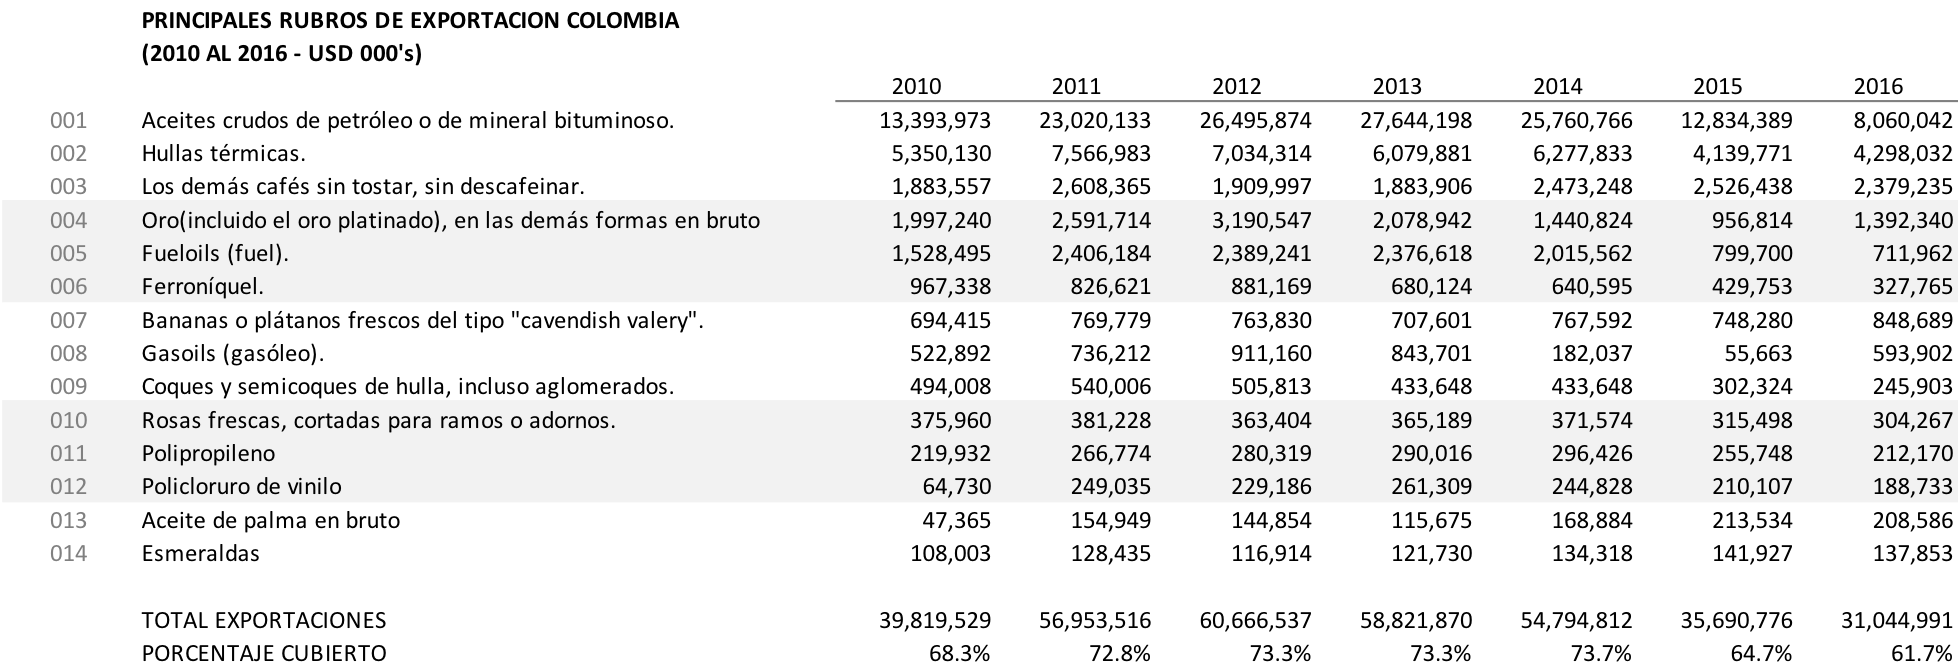
\includegraphics[width = 15cm]{ExportacionesColombia.png}
\caption{Principales Rubros de Exportación Colombia 2010-2016}
\end{figure}

\section{Regresión Lineal}
La regresión lineal es el punto de entrada más sencillo de entender y aplicar en la Ciencia de Datos. Parte de esto se debe a que la regresión lineal es aplicable en muchos casos a una gran gama de problemas de predicción en los cuales el científico de datos cuenta con una base de datos o juego de datos lo suficientemente grande y accesible para entrenar un modelo \cite{daroczi}. La segunda razón es que un modelo bien entrenado de regresión lineal por lo general nos da una respuesta con cierto grado de precisión que da por cerrado el caso \cite{leek}.

El concepto en sí es relativamente sencillo de abstraer y explicar. En una visualización de datos donde un valor $y$ se corresponde con alguna relación del valor $x$, para cada $x$ y $y$, es posible trazar una línea que en cierta forma sea representativa del valor de predicción de $y$ para cada $x$. Esta línea puede no ser perfecta, o puede dejar muchos puntos sin una relación válida (a menos en el papel de gráfico) pero nos da una idea aproximada de la tendencia y evolución de los datos. \\

\begin{figure}[h!]
    \centering
    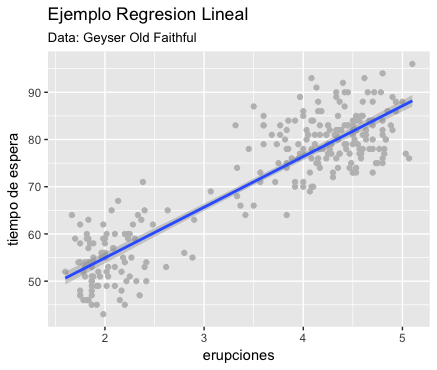
\includegraphics[width = 4 in]{ejemRegresionLineal.png}
    \caption{Ejemplo de Regresión Lineal con Old Geyser}
\end{figure}

Zumel y Mount describen la regresión lineal como el más común de los métodos de aprendizaje automatizado \cite{zumelMount}. Para los autores hay una probabilidad muy grande que el método funcione bien con el problema, y si no, es muy fácil verificar cual otro método probar como segunda opción. Para Daroczi, el énfasis está en los modelos de regresión multivariable (una extensión de la regresión lineal simple de un solo predictor y resultado) que construyen el camino para la predicción de fenómenos complejos en la naturaleza y negocios \cite{daroczi}. Por su parte, Harrington resume los beneficios de la regresión lineal \cite{harrington} por la facilidad de interpretar los resultados y lo frugal en el uso de ciclos de computación (aunque puede ser menos útil si el fenómeno no es perfectamente lineal).

\subsection{Definición de Regresión Lineal}
Downey describe la regresión lineal como aquella que está basada en modelos de funciones lineales \cite{thinkStats}. Para Mann y Lacke la regresión lineal es aquella que se da como una función lineal entre dos variables, y la cual se puede dibujar en el plano cartesiano como una recta \cite{intoStats7}. Yau por su lado, define la regresión lineal simple como el modelo que describe la relación entre dos variables, $x$ y $y$, expresada por la ecuación de regresión lineal, donde $\alpha$ y $\beta$ son parámetros y $\epsilon$ es el término de error \cite{yau}. Para García, López y Calvo, el primer paso para el estudio de la relación entre las variables consiste en la construcción y observación de un diagrama de dispersión. El problema de la regresión se concreta entonces en ajustar una función a la nube de puntos representada en dicho diagrama. Esta función permitirá entonces obtener, al menos de forma aproximada, una estimación del valor de una de las variables a partir del valor que tome la otra \cite{estadisticaBasica}.

La fórmula a la que hacemos referencia en la definición de Yau, y la que utilizan los otros autores, es la siguiente:

\begin{equation}
	Y_{i} = \beta_{0} + \beta_{1}X_{i} + \epsilon_{i}
\end{equation}

Dentro del aprendizaje automatizado la regresión tiene su propia interpretación donde se asume que el modelo está definido por un juego de parámetros \cite{alpaydin}:

\begin{equation}
	y = g(x \mid \theta)
\end{equation}

donde $g(.)$ es el modelo y $\theta$ son sus parámetros. $Y$ es un número dentro de una regresión y $g(.)$ es la función de la regresión. El programa de aprendizaje automatizado optimiza los parámetros $\theta$ de forma que el error de aproximación sea mínimo, o en otras palabras, que los valores estimados sean los más cercanos a los valores reales del juego de entrenamiento.

Los parámetros $\beta_{0}$ y $\beta_{1}$ determinan el punto en el que la función intercepta la la ordenada y la pendiente de la función. Podemos profundizar estos dos puntos aún más:
\begin{itemize}
	\item el punto de intercepción es la predicción del valor de $y$ cuando $x=0$.
    \item la pendiente $\beta_{1}$ representa la predicción del aumento de $y$ con cada unidad que incrementa $x$
\end{itemize}

Notemos que las observaciones no están dispuestas en una línea recta, sino que se encuentran dispersas alrededor de esta. Debemos pensar de cada observación $\beta_{0} + \beta_{1}x_{i}$ como la parte sistemática del modelo, y $\epsilon_i$ como el error aleatorio. Este margen de error no es un error per se, pero una desviación del modelo lineal \cite{hyndman}. Asumimos que el factor de error cumple con los siguientes requisitos.

\begin{enumerate}
  \item tiene media cero
  \item no contiene autocorrelación
  \item no está relacionado con la variable predictor
\end{enumerate}

Se espera que la distribución de los errores sea normal con varianza constante para producir pronósticos precisos.

\subsection{Estimación con Mínimos Cuadrados}
En la práctica se tiene un juego de valores y no los mismos de $\beta_{0}$ y $\beta_{1}$. Estos necesitan ser calculados en base al juego de datos en lo que se conoce como el calce o ajuste de la linea a través de los datos. Hay muchas posibles líneas que calcen en el modelo con diferentes valores para $\beta_{0}$ y $\beta_{1}$. El método de mínimos cuadrados provee una forma de seleccionar valores para $\beta_{0}$ y $\beta_{1}$ minimizando la suma del error cuadrático \cite{estadisticaBasica}:

\begin{equation}
	\sum_{i=1}^{N} \epsilon_{i}^{2} = \sum_{i=1}^{N}(y_{i} - \beta_{0} - \beta_{1}x_{i})^2
\end{equation}

Utilizando cálculo matemático, se ha demostrado que los estimados de los mínimos cuadrados son:

\begin{equation}
\begin{split}
	\hat{\beta}_{1} &= \frac{\sum_{i=1}{N}(y_{i}-\bar{y})(x_{i} - \bar{x})}{\sum_{i=1}{N}(x_{i}-\bar{x})^2}\\
	\hat{\beta}_{0} &= \bar{y} - \hat{\beta}_{1} \bar{x}\\
\end{split}
\end{equation}

\subsection{Limitaciones de la Regresión Lineal}
Aunque el análisis de la regresión lineal y la derivación del coeficiente de correlación parecen un método muy adecuado para estudiar la relación entre dos variables, hay que indicar que tiene importantes debilidades \cite{estadisticaBasica}. En particular:

\begin{itemize}
	\item Tanto la recta de regresión como el coeficiente de correlación no son robustos, en el sentido de que resultan muy afectados por medidas particulares que se alejen mucho de la tendencia general.
	\item No hay que olvidar que el coeficiente de correlación no es más que una medida resumen. En ningún caso puede substituir al diagrama de dispersión, que siempre habrá que construir para extraer más información. Formas muy diferentes de la nube de puntos pueden conducir al mismo coeficiente de correlación.
	\item El que en un caso se obtenga un coeficiente de correlación bajo no significa que no pueda existir correlación entre las variables. De lo único que nos informa es de que la correlación no es lineal (no se ajusta a una recta), pero es posible que pueda existir una buena correlación de otro tipo.
	\item Un coeficiente de correlación alto no significa que exista una dependencia directa entre las variables. Es decir, no se puede extraer una conclusión de causa y efecto basándose únicamente en el coeficiente de correlación. En general hay que tener en cuenta que puede existir una tercera variable escondida
	que puede producir una correlación que, en muchos casos, puede no tener sentido.
\end{itemize}

\subsection{Regresión Multi-Variable}
Para Downey \cite{thinkStats}, la regresión múltiple es aquella en la cual se utilizan múltiples variables independientes, pero una sola variable dependiente.

El Dr. Tattar de la Universidad de Bangalore define que el modelo de regresión línea simple no es realista ni aplicable al mundo practico \cite{narayanachar}. Para aplicaciones más reales, es casi obligatorio el uso de modelos de regresión múltiple, en los cuales varias variables independientes se conjugan como parámetros de regresión.

La regresión multivariable no es un tema mayormente complicado en teoría cómo lo es en llevar a la práctica. No todos los ejemplos de regresiones multivariables nos van a llevar a funciones lineales, sino que estamos tocando el limite entre regresión lineal y métodos de regresión general con funciones no lineales que pueden necesitar de transformaciones matemáticas para obtener un modelo apropiado \cite{daroczi}. Aquí también se explica la selección de un modelo con múltiples variables independientes y cuales conviene seleccionar \cite{viswanathan}.

La mayor parte de la teoría de esta sección sigue el desarrollo de la fórmula:

\begin{equation}
	Y_{i} = \beta_{0} + \beta_{1}X_{1} + \beta_{2}X_{2} + \cdots + \epsilon_{i}
\end{equation}

Para medir el nivel de relación entre una variable de predicción y otra de respuesta sobra el modelo de regresión lineal tradicional. Pero si se trata de modelos modelos más complejos donde una serie de variables pueden estar afectando el resultado, es necesario utilizar un modelo multivariable. Una variable oculta \cite{estadisticaBasica} o confundidora \cite{daroczi} es aquella que sesga (incrementa o disminuye) el valor de la asociación que se analiza. En este sentido una variable confundidora siempre está asociada con la respuesta y el predictor. Los modelos de regresión en general se entienden como formas de medir la asociación entre respuestas y predictores controlando el efecto de terceros. Confundidores potenciales se agregan al modelo como predictores adicionales, y el coeficiente de regresión del predictor (el coeficiente parcial) mide el efecto de la regresión ajustada por los confundidores \cite{daroczi}.

\subsection{Presunción del Modelo}
Los modelos de regresión lineal que utilizan los métodos tradicionales de estimación hacen un número de presunciones sobre el resultado de las variables estimadas, las variables regresores, y su relación \cite{daroczi}.

\begin{enumerate}
    \item $Y$ es una variable continua (no es binaria, nominal u ordinal)
    \item La variación aleatoria (los errores residuales) son estadísticamente independientes
    \item Existe una relación estocástica lineal entre $Y$ y cada $X$
    \item $Y$ tiene una distribución normal, si tomamos $X$ fijo
    \item $Y$ tiene la misma varianza, más allá del valor fijo de las $X's$
\end{enumerate}

Una violación del precepto 2 ocurre en el análisis de series de tiempo, si se utiliza el tiempo como variable de predicción. Dado que los años consecutivos no son independientes, el error no será independiente tampoco. Una violación del precepto 3 ocurre cuando la relación no es exactamente lineal sino que existe una desviación de la linea de tendencia. Los preceptos 4 y 5 requieren que la distribución condicional de $Y$ sea normal y tenga la misma varianza, sin importar los valores correspondientes de las $X's$. Finalmente el precepto 5 se conoce como \emph{homocedasticidad}, y en caso contrario la regresión se ve afectada por el efecto de \emph{heterocedasticidad}.

\subsection{Calce de los Datos}
Llegar a un modelo de regresión lineal no significa llegar a una solución óptima, ni mucho menos. Los datos pueden calzar de forma muy elástica dentro del modelo, por lo que debemos recurrir a ciertas medidas para verificar si el modelo tiene algún poder predictivo de uso científico. Decimos que existe una correlación lineal en el grado en que la nube de puntos representada en el diagrama de dispersión se acerca a una recta. Cuanto mejor se aproxime dicha nube a una recta, mayor será el grado de correlación lineal \cite{estadisticaBasica}. De esta forma, el estudio de la correlación lineal está íntimamente ligado al de la regresión lineal. Distinguiremos dos tipos de correlación lineal. Cuando al crecer la variable x, la variable y tienda también a aumentar (pendiente positiva de la recta de regresión) diremos que tenemos una correlación positiva o directa. Cuando ocurra lo contrario, la correlación será negativa o inversa \cite{estadisticaBasica}.

\subsubsection{Covarianza de una Correlación Lineal}
Evidentemente, la simple observación del diagrama de dispersión proporciona una idea cualitativa del grado de correlación. Sin embargo, es claramente más útil disponer de una medida cuantitativa de dicha correlación. Una primera cuantificación de la correlación se puede obtener a partir de la covarianza. Puede observarse que, en el caso de una clara correlación lineal positiva, la mayor parte de los puntos de datos estarán en el segundo y tercer cuadrante, de forma que, cuando $x_i$ sea mayor que $\bar{x}$, también $y_i$ tenderá a ser mayor que $y$, y al revés. Por tanto, la mayoría de los términos del sumatorio serán positivos y la covarianza alcanzará un valor alto. Por el mismo argumento, si existe correlación lineal negativa, la mayoría de los términos del sumatorio serán negativos y la covarianza tendrá un valor alto y negativo. En el caso de que no hubiese correlación y los puntos estuviesen repartidos en los cuatro cuadrantes, aparecerían por igual términos positivos y negativos, que se anularían dando un valor muy bajo, en valor absoluto, de la covarianza. En resumen, la covarianza es una medida de la correlación lineal entre las dos variables \cite{estadisticaBasica}.

\subsubsection{R - Coeficiente de Correlación de Pearson}
La utilidad de la covarianza como medida de correlación está limitada por el hecho de que depende de las unidades de medida en que se trabaje. Para construir una medida adimensional de la correlación habrá que dividir la varianza por un término con sus mismas dimensiones. De esta forma, se define el \emph{coeficiente de correlación lineal R} como el cociente entre la covarianza y las desviaciones típicas (o raíces cuadradas de las varianzas) de $x$ e $y$ \cite{estadisticaBasica}.

El coeficiente de correlación también se conoce como \emph{coeficiente de correlación de Pearson} mide la relación lineal entre dos variables aleatorias cuantitativas. La correlación de Pearson es independiente de la escala de medida de las variables, lo que permite tener comparaciones mucho más objetivas independiente del fenómeno estudiado. De manera menos formal, podemos definir el coeficiente de correlación de Pearson como un índice que puede utilizarse para medir el grado de relación de dos variables siempre y cuando ambas sean cuantitativas \cite{intoStats7}.

\begin{equation}
    R = \frac{\Sigma(x_i - \bar{x})(y_i - \bar{y})}{\sqrt{\Sigma(x_i - \bar{x})^2\Sigma(y_i - \bar{y})^2}}
\end{equation}

\subsubsection{R2 - Coeficiente de Determinación}
El coeficiente de determinación - denominado \(R^{2}\) - es un estadístico usado en el contexto de un modelo estadístico cuyo principal propósito es predecir resultados futuros o probar una hipótesis. El coeficiente determina la calidad del modelo para replicar los resultados, y la proporción de variación de los resultados que puede explicarse por el modelo \cite{daroczi}. El coeficiente de determinación, puede interpretarse como la fracción de la variación total que se explica por la recta de regresión. Así, un coeficiente de correlación próximo a +1 o -1 indica que casi todas las variaciones encontradas en $y$ son explicadas por la recta (teniéndose una buena correlación), mientras que si $R$ es 0, la recta de regresión apenas sirve para explicar las variaciones y la correlación lineal será pobre. Como ejemplo, si $R = 0.95$, podemos deducir que aproximadamente el 90\% de las variaciones de $y$ son debidas a la regresi'on lineal.

En el caso de regresión lineal, la formula del coeficiente de determinación sigue la siguiente forma:

\begin{equation}
    R^{2} = \frac{\sigma^{2}_{XY}}{\sigma^{2}_{X}\sigma^{2}_{Y}}
\end{equation}

\subsection{Valor de p}
La evaluación de una hipótesis emerge como un componente crucial en la toma de decisión cuando dos opciones compiten como solución de un problema. La evaluación estadística de la hipótesis provee un marco formal y guías para hacer tal selección \cite{thinkStats}. Una hipótesis estadística es una afirmación o conjetura que se hace sobre una, o varias, características de una población. Ejemplos de dichas afirmaciones incluyen el que la media de una población tenga un determinado valor, o que los valores de una variable presenten menor dispersión en torno a un valor medio en una población comparada con la dispersión en otra, etc. Evidentemente, la forma m´as directa de comprobar tales hipótesis sería estudiando todos y cada uno de los elementos de la población. Sin embargo, frecuentemente esto no es posible (la población podría ser incluso infinita), por lo que el contraste de la hipótesis ha de basarse en una muestra, que supondremos aleatoria, de la población en estudio. Al no estudiarse la población entera, nunca podremos estar completamente seguros de si la hipótesis realizada es verdadera o falsa. Es decir, siempre existe la probabilidad de llegar a una conclusión equivocada \cite{estadisticaBasica}.

Una prueba estadística de hipótesis está formada de cinco partes \cite{mendehall}:

\begin{enumerate}
    \item La hipótesis nula, denotada por $H_0$
    \item La hipótesis alternativa, denotada por $H_a$
    \item El estadístico de prueba y su valor $p$
    \item La región de rechazo
    \item La conclusión
\end{enumerate}

Las dos hipótesis en competencia son la hipótesis alternativa $H_a$, generalmente la hipótesis que el investigador desea apoyar y la hipótesis nula $H_0$, una contradicción de la hipótesis alternativa. Es más fácil presentar apoyo para la hipótesis alternativa al demostrar que la hipótesis nula es falsa. En consecuencia, el investigador estadístico siempre empieza por suponer que la hipótesis nula $H_0$ es verdadera. El investigador utiliza entonces los datos muestrales para decidir si la evidencia está a favor de $H_a$ más que de $H_0$ y saca una de dos conclusiones:

\begin{itemize}
    \item Rechaza $H_0$ y concluye que Ha es verdadera.
    \item Acepta (no rechaza) $H_0$ como verdadera
\end{itemize}

La decisión de rechazar o aceptar la hipótesis nula está basada en información contenida en una muestra sacada de la población de interés. Esta información toma estas formas:

\begin{itemize}
    \item \textbf{Estadística de prueba:} un solo número calculado a partir de los datos muestrales
    \item \textbf{Valor p:} probabilidad calculada usando la prueba estadística
\end{itemize}

Cualquiera de estas mediciones, o ambas, actúan como quienes toman decisiones para el investigador al decidir si rechazar o aceptar H0 \cite{mendehall}. Un valor de $p$ por debajo de 0.05 puede interpretarse como que la regresión es estadísticamente significativa \cite{daroczi}.

\section{Series de Tiempo}
Muchos autores han escrito sobre las series de tiempo, pero es difícil agregar al tema o discutir las ideas del profesor Robert Hyndman, uno de los expertos más respetados en la comunidad de la estadística por su trabajo en las series de tiempo. Hyndman extiende la teoría a las series de tiempo como elementos de pronostico y su relación con la regresión lineal \cite{hyndman}. Desde el punto de vista técnico, Hyndman es el creador de varias bibliotecas de funciones de pronostico utilizando series de tiempo y ARIMA en lenguaje R. Dentro de la bibliografía, Daroczi es quien agrega detalles sobre la detección temprana de valores atípicos que pueden dificultar – y mucho – el análisis \cite{daroczi}. 

\subsection{Introducción a las Series de Tiempo}
Las series de datos son muy útiles para pronosticar algo que cambia con el tiempo. Ejemplos de estas cantidades que varían con el tiempo incluyen acciones en la bolsa de valor, cifras de ventas, y otro tipo de información cuantitativa \cite{hyndman}.

Una serie de tiempo es una serie de datos indexada en orden temporal. Comúnmente una serie de datos es una secuencia de datos tomados a puntos sucesivos y equidistantes en el tiempo, lo que la convierte en una secuencia de datos discretos en el tiempo. En forma general cualquier cosa que observamos secuencialmente en el tiempo es una serie de tiempos \cite{hyndman}. La literatura académica se concentra en series de tiempo que se observan en intervalos regulares de tiempo, aunque aquellas que se observan en intervalos irregulares también existen. 

El análisis de las series de tiempo es el uso de métodos para extraer estadísticas interesantes y otras características de los datos. El pronóstico de series de tiempo es el uso de modelos para predecir valores futuros basados en valores observados en el pasado. En el pronóstico de series de tiempo, la idea principal es estimar cómo la secuencia de observaciones continuará en el futuro. El pronóstico de series de tiempo utiliza solamente información de la variable a ser pronosticada, y no hace intento alguno de descubrir cuales son los factores que motivan este comportamiento (en análisis de regresión diríamos que buscamos las variables de confusión). Por lo tanto el análisis de series de tiempo extrapola la tendencia secular y los patrones cíclicas, pero ignora todo otro tipo de información que puede afectar el movimiento de la variable estudiada, como pueden ser en la vida real efectos de la publicidad en el lanzamiento de un producto, la tasa de cambio en las ventas, o actividades de riesgo en el precio internacional de materias primas. 

Podemos ver un ejemplo de serie de tiempo si tomamos los valores de la TRM (la Tasa Representativa de Mercado, el nombre oficial de la tasa de cambio del dólar en Colombia) en la siguiente gráfica:

\begin{figure}[h]
    \centering
    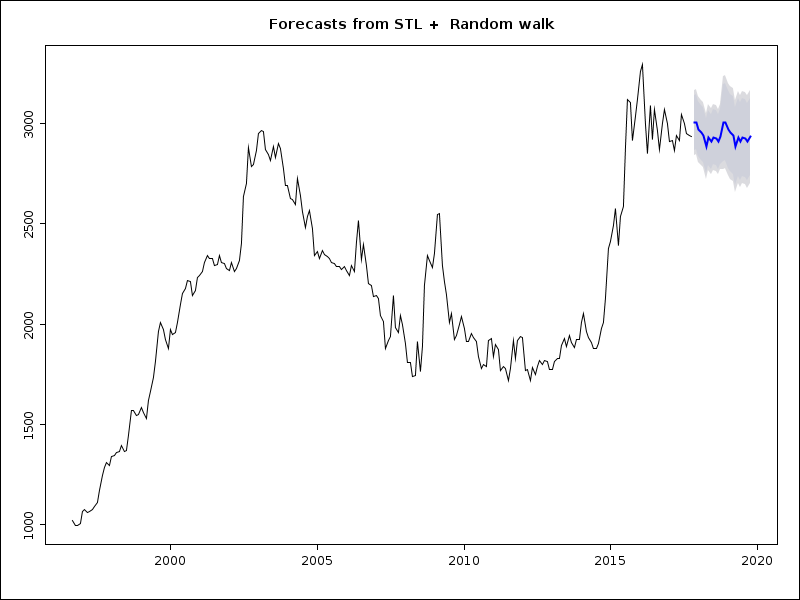
\includegraphics[width = 4 in]{timeSeries1.png}
    \caption{Ejemplo de Pronóstico con Descomposición STL (Fuente Hyndman and Athanasopoulos)}
\end{figure}

La línea negra es la variación de la TRM a lo largo del tiempo (en este caso, desde el año 1980 hasta el 2017). La línea azul es el pronóstico del valor de la TRM según la función \texttt{forecast()} del lenguaje R. La zona gris comprenden el intervalo de confianza del pronóstico, la cual nos da una idea más real de como puede fluctuar el pronóstico dentro del mismo.

La forma de una ecuación de series de tiempo se puede escribir en los siguientes términos:

\[ x(t+1) = f(x_t, x_{t-1}, x_{t-2}, \ldots, error) \]

Es posible utilizar predictores en el pronóstico de series de tiempo. Un ejemplo utilizando el tema de investigación de este mismo trabajo es el pronóstico de la TRM, la cual estimamos es el resultado de varios factores:

\[ TRM = f(\textnormal{demanda dólar, tasa interés, turismo, error}) \]

La relación no es exacta, sino que siempre habrá factores por lo cuales el modelo no puede responder. Estas variaciones están previstas en el término error dentro del modelo. Este tipo de modelo se llama \emph{modelo explanatorio}. 

Las series de tiempo se suelen catalogar en aditivas y multiplicativas. 

\begin{itemize}
	\item Las series aditivas son aquellas cuya variación en la estacionalidad, o variación en el ciclo o tendencia secular, no aumentan de forma proporcional al avance del tiempo.
	\item Las series multiplicativas son aquellas cuya variación en la estacionalidad, o variación en el ciclo o tendencia secular, aumentan de forma proporcional al avance del tiempo. Las series multiplicativas son comunes en ciencias como la economía y finanzas.
\end{itemize}

\subsection{Pronóstico con Series de Tiempo}
Los pronósticos con series de tiempo utilizan solamente la información disponible de la variable que se propone pronosticar, sin hacer intento alguno por descubrir los factores adicionales que condicionan su comportamiento. Por lo tanto se extrapolan las tendencias y patrones temporales, pero se ignora toda la información adicional como pueden ser iniciativas de publicidad, actividad de la competencia, cambios en las condiciones económicas y otros \cite{hyndman}.

\subsection{Patrones}
Las series de tiempo pueden descomponerse según su patrón o tendencia en tres elementos que las componen [Velazco, M., 2017]. A saber:

\begin{enumerate}
	\item Tendencia Secular: la tendencia secular o tendencia a largo plazo de una serie de tiempo es por lo común el resultado de factores a largo plazo. La tendencia no tiene porque ser lineal. Además es común ver que la tendencia cambia de dirección, ascendente o descendente \cite{hyndman}.
	\item Variación Estacional: Es el componente de la serie de tiempo que representa la variabilidad de los datos debido a la influencia de las estaciones. El componente de estacionalidad es siempre fijo \cite{hyndman}
	\item Variación Irregular: Esta variación se debe a factores a corto plazo, imprevisibles, y no recurrentes que afectan la serie de tiempo. Algunos autores llaman a estas variaciones \emph{cíclicas}. 
\end{enumerate}

Es importante saber distinguir entre los patrones cíclicos y estacionales. Los patrones estacionales tienen una duración fija y conocida en su extensión, mientras que los patrones cíclicos son mucho más extensos que los patrones estacionales y la duración de su magnitud es variable. La forma más sencilla es identificar los ciclos de estación con el calendario, por ejemplo los aumentos de tráfico en los centros comerciales en las fiestas de fin de año \cite{hyndman}. 

\subsection{Auto Correlación}
De igual manera que una correlación mide la extensión de una relación lineal entre dos variables, la autocorrelación mide la relación lineal entre dos valores retrasados de series de tiempo \cite{hyndman}.

El valor de una autocorrelación para un \(r_{k}\) dado es:

\[ r_{k} = \frac{\sum_{t = k + 1}^T(y_{t} - \bar{y})(y_{t - k} - \bar{y})}{\sum_{t = 1}^T(y_{t} - \bar{y})^{2}} \]

donde \(T\) es el valor de período temporal de la serie de tiempo. 

El autor Daroczi agrega como metodología para la verificación de autocorrelación en un juego de datos (no solo una serie de tiempos, sino cualquier juego de datos espacial) el \emph{Indice I de Moran} \cite{daroczi}. Dicho índice esta dado por la formula:

\[ I = \frac{N}{W} 
	\frac{\sum{i}\sum{j}w_{ij}(x_{i} - \bar{x})(x_{j} - \bar{x})}{{\sum{i}(x_{i} - \bar{x})^2}} \]

Los coeficientes de autocorrelación se visualizan a través de un gráfico de la función de autocorrelación o ACF (también llamado correlograma). Dicho gráfico analiza las relaciones entre valores retrasados de la serie de tiempo. Podemos utilizar la serie de tiempo representativa de la TRM para visualizar su gráfica de ACF.

\begin{figure}[h!]
    \centering
    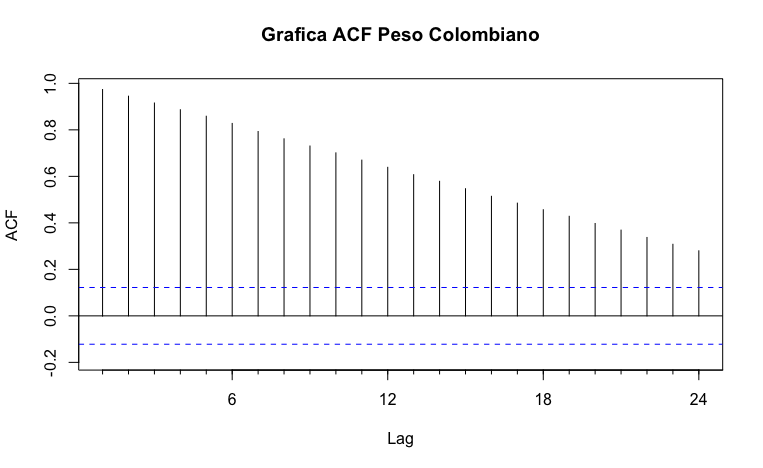
\includegraphics[width = 4 in]{COPEjemploACF.png}
    \caption{Correlograma del Peso Colombiano (Fuente propia)}
\end{figure}

Las series de tiempo que no muestran efectos de autocorrelación se denominan \emph{ruido blanco}. En dichas series se espera que los coeficientes de correlación sean cercanos a cero. Esto de por si es difícil, ya que toda serie de tiempo tendrá cierta variación aleatoria, pero en términos matemáticos esperamos que la serie tenga variaciones que 95\% del tiempo estén dentro de la región de $\pm2/\sqrt{T}$ donde $T$ es la extensión de la serie de tiempo. Si hay una o más series de magnitud fuera de estos límites, o si el 5\% o más de las series están fuera de estos límites, es muy probable que no sea ruido blanco \cite{hyndman}.

Existe una prueba adicional de autocorrelación que utiliza todo un grupo de datos $r_k$ en vez de tratarlos por separado. El racional para el proceso es que la visualización normal de una gráfica ACF es un test de hipótesis para cada retraso entre series. Cuando se hacen múltiples de estos test, la probabilidad de encontrar un falso positivo incrementa. Se evita este problema evaluando si las autocorrelación de los primeros $h$ valores es diferente de una serie de ruido blanco. El test de un grupo de valores con autocorrelación se conoce como un test \emph{portmanteau}. Uno de los más utilizados es el test \emph{Box-Pierce}:

\[ Q = T \sum_{k=1}^{h}r_{k\prime}^2 \]

donde $h$ es el retraso máximo considerado y $T$ es el número de observaciones. Si cada uno de los $r_k$ es cercano a cero, entonces Q sera mínimo. Si alguno de los valores de $r_k$ son grandes (ya sea positivos o negativos), entonces Q será grande. Hyndman y Athanasoupulos sugieren utilizar $h = 10$ para data no estacional y $h = 2m$ para datos con estacionalidad, donde $m$ es el número de estaciones, por ejemplo 4 para trimestres \cite{hyndman}.  El test \emph{Box-Pierce} tiende a no ser confiable con valores grandes de $h$. Si $h > T/5$ es recomendable utilizar $h=T/5$.

Un test relacionado - y más preciso - es el test \emph{Ljung-Box}:

\[ Q* = T(T+2) \sum_{k=1}^{h}(T-k)^{-1}r_{k\prime}^{2} \]

Si el valor de $Q*$ es grande, las autocorrelaciones no provienen de una serie de ruido blanco. 

\subsection{Precisión del Pronóstico}
Para el estudio de la precisión del pronóstico de series de tiempo, sea $y_i$ la observación $i$ de datos y $\hat{y_i}$ el pronóstico de $y_i$.

\subsubsection{Errores dependiente de la Escala}
El error del pronóstico es la diferencia $e_i = y_i - \hat{y_i}$, que está en la misma escala que los datos. Las medidas de precisión que dependen de $e_i$ son dependientes de la escala y no se pueden utilizar para hacer comparaciones entre series de tiempo de diferentes escalas. Las dos formas que se utilizan comúnmente para medir la precisión del pronóstico de series de tiempo dependiente de escalas están basadas en el error absoluto o error cuadrático \cite{hyndman}. Se trata de:

\begin{eqnarray*}
	\text{Error Promedio Absoluto (MAE)}& = &\text{promedio}(|e_{i}|) \\
	\text{Error Promedio Cuadrático (RMSE)}& = &\sqrt{promedio_{e_1}^2} 
\end{eqnarray*}

La tendencia al comparar precisión en un solo juego de datos es utilizar el MAE ya que es mas sencillo y simple de entender. 

\subsubsection{Errores Porcentuales}
Un error porcentual es del tipo $p_i = 100 e_i / y_i$. Los errores porcentuales son independientes de la escala, y se utilizan con facilidad para comparar errores en la precisión de múltiples juegos de datos. Es error porcentual más común es:

\[ \text{Error Promedio Porcentual Absoluto (MAPE)} = promedio(\mid p_i \mid) \]

Las medidas basadas en errores porcentuales tienen la debilidad de ser infinitas o indefinidas cuando $y_i = 0$ para cualquier $i$. Esto también ocurre cuando un $y_i$ tiende a cero. 

\subsection{Descomposición de Series de Tiempo}
La descomposición de las series de tiempo facilita el análisis y la investigación exploratoria de los datos. Una de las formas mas sencillas de lograr esto es la aplicación de promedios móviles, lo cual se facilita mucho en R con el uso de la función \texttt{decompose()} \cite{daroczi}.

Pensemos en la serie de tiempo $y_t$ compuesta por tres factores: un componente estacional, un componente de tendencia (que contiene tanto tendencia secular como cíclica) y un último componente que contiene cualquier otro resto de información importante. Podemos entonces escribir una serie de tiempos aditiva como:

\[ y_t = S_t + T_t + E_t \]

donde $y_t$ es la data en el período $t$, $S_t$ es el componente estacional en el período $t$, $T_t$ es el componente de tendencia-ciclo en el período $t$, y $E_t$ es el componente de error en el período $t$. De forma alternativa podemos escribir una ecuación similar para los modelos de series de datos multiplicativos como:

\[ y_t = S_t * T_t * E_t  \]

El modelo aditivo es más apropiado si la magnitud de las fluctuaciones estacionales o la variación alrededor del ciclo o tendencia no varía con los niveles de la serie de tiempo (ejemplo: el avance del tiempo). Cuando la variación se da, o sea es proporcional con el avance del tiempo en la serie, un modelo multiplicativo es más apropiado. Este es el caso de la mayoría de las series de tiempo en la economía \cite{hyndman}.

\subsubsection{Datos Ajustados Estacionalmente}
Si el componente de estacionalidad se elimina de la serie de datos original, los valores resultantes se denominan \emph{ajustados estacionalmente}. Para un modelo aditivo, el ajuste por estacionalidad se da por $y_t - S_t$. Para un modelo multiplicativo este se da por $y_t/S_t$. Si la variación por estacionalidad no es de importancia, la serie ajustada por estacionalidad puede ser útil. Estos casos se dan por ejemplo con los datos de desempleo mensual, los cuales se saben tienen variación estacional que altera la lectura real del cambio. 

\subsubsection{Métodos de Descomposición de Series de Tiempo}
Existen múltiples métodos de descomposición de series de tiempo. En nuestro marco teórico tocaremos brevemente los de promedios móviles, promedios móviles ponderados, STL, suavizar exponencialmente, y ARIMA.

\subsubsection{Promedios Móviles}

El método de promedios móviles origina de los años 1920 y fue ampliamente utilizado hasta los 1950. Hasta el día de hoy es la base de todos los otros métodos modernos de descomposición. El fundamento del mismo es utilizar los promedios móviles para estimar la tendencia o ciclo \cite{hyndman}. La descomposición por promedios móviles toma la forma siguiente:

\[ \hat{T}_{t} = \frac{1}{m} \sum_{j = -k}^{k} y_{t + j}  \]

donde $m=2k+1$. Esto significa que el estimado de la tendencia/ciclo en el momento $t$ se obtiene promediando los valores de la serie de tiempo dentro de $k$ períodos de $t$ valores. 

\subsubsection{Promedios Móviles Ponderados}
Es posible obtener promedios móviles de los promedios móviles. Combinaciones de estos nos dan promedios ponderados. Por ejemplo un modelo 2X4-MA, que es un promedio de promedios móviles, es el equivalente a un modelo 5-MA con ponderaciones dadas por el vector de pesos $[\frac{1}{8}, \frac{1}{4}, \frac{1}{4}, \frac{1}{4}, \frac{1}{8}]$ \cite{hyndman}. La forma de escribir un modelo de promedios móviles ponderados es la siguiente:

\[ \hat{T}_{t} = \sum_{j = -k}^{k} a_j y_{t + j}  \]

donde $k=(m-1)/2$ y los pesos están dados por $[a_{-k}, \ldots, a_{k}]$. Es importante que todos los pesos sumen uno como valor y que sean simétricos para que $a_{j} = a_{-j}$. Una ventaja mayor de los promedios móviles ponderados es que producen estimados más suavizados de la tendencia/ciclo. 

\subsubsection{Descomposición STL}
El método STL es muy versátil y robusto para la descomposición de series de tiempo. Su nombre es el acrónimo en inglés de \emph{Seasonal and Trend Descomposition using Loess}, que significa descomposición de estacionalidad y tendencia utilizando Loess. Loess es un método para estimar relaciones no-lineales desarrollado por Cleveland et al \cite{hyndman}. Las desventajas de STL es su manejo de cierta data financiera (como por ejemplo días de comercio bursátil) y las variaciones de calendario. La biblioteca de R tiene una función que descompone automáticamente una serie de datos utilizando STL, la función \texttt{STL()}.

La descomposición STL se utiliza más que nada para estudiar las series de tiempo, pero tiene aplicación en pronosticar. Asumiendo una descomposición aditiva, la serie de tiempo descompuesta se puede escribir como:

\[ y_{t} = \hat{S}_t + \hat{A}_t \]

donde $\hat{A}_t = \hat{T}_t + \hat{E}_t$ es el componente ajustado por estacionalidad. Si se trata de una serie multiplicativa entonces la misma ecuación se puede escribir como: 

\[ y_{t} = \hat{S_t}\hat{A_t}\]

donde $\hat{A}_t = \hat{T}_t\hat{E}_t$. 

Para pronosticar cualquier componente ajustado por estacionalidad, se puede utilizar cualquier método de pronóstico no estacional. Por ejemplo, se puede aplicar camino aleatorio con deriva, Holts-Winter, o ARIMA.

\subsubsection{Alisamiento Exponencial}
El Alisamiento Exponencial (o Suavizamiento Exponencial según la traducción), fue propuesto por Brown, Holt y Winters entre los años 1950 a 1960. Los pronósticos producto del suavizamiento exponencial son promedios ponderados de observaciones históricas en las cuales el valor del peso va decayendo a medidas que las observaciones van envejeciendo. En otras palabras, las observaciones más nuevas reciben mayor asociación con el peso. 

La primera forma de suavizamiento exponencial se llama \emph{suavizamiento exponencial simple}. Este método es aplicable para el pronóstico de series de datos sin tendencia o estacionalidad. El pronostico se calcula con promedios ponderados donde los pesos decrecen exponencialmente a medida que las observaciones envejecen - los pesos más pequeños se asocian con las observaciones más antiguas. 

\[ \hat{y}_{T+1 \mid T} = \alpha y_{T} + \alpha(1-\alpha) y_{T-1} + \alpha(1-\alpha)^2 y_{T-2} + \alpha(1-\alpha)^3 y_{T-3} + \ldots \]

donde $0 \leq \alpha \leq 1$ es el parámetro de alisamiento. El pronóstico de $T + 1$ es el promedio ponderado de todas las observaciones en la serie $y_1, \ldots, y_T$. La tasa por la cual decrecen los pesos se controla con el parámetro $\alpha$.

Este método se puede extender aplicando el factor de suavizamiento exponencial decreciente para lograr la ecuación de la segunda forma de suavizamiento exponencial ponderado de tal forma que:

\[ \hat{T}_{T+1 \mid T} = \sum{j=0}^{T-1} \alpha(1-\alpha)^j y_{T-j} + (1-\alpha)^{T} \ell_{0}  \]

Notemos que la ecuación es otra forma de escribir la notación del suavizamiento exponencial simple. 

Holt extendió el método de suavizamiento exponencial para permitir hacer pronósticos con datos que contenían tendencia \cite{hyndman}. Este método de pronóstico incluye una ecuación de pronóstico y dos ecuaciones de suavizamiento, una para el nivel y otra para la tendencia:

\begin{eqnarray*}
	\text{Ecuación de Pronóstico}&&\hat{y}_{t+h \mid t} = \ell_{t} + hb_{t} \\
	\text{Ecuación de Nivel}&&\ell_{t} = \alpha y_{t} + (1 - \alpha)(\ell_{t-1} + b_{t-1}) \\
	\text{Ecuación de Tendencia}&&b_{t} = \beta^{*}(\ell_{t} - \ell_{t-1}) + (1 - \beta^{*})b_{t-1}  
\end{eqnarray*}

donde $\ell_{t}$ denota el nivel estimado de la serie de tiempo en el momento $t$, $b_{t}$ denota el estimado de la tendencia de la serie de tiempo en el momento $t$, $\alpha$ es el parámetro de suavizamiento para el nivel, $0 \lq \alpha \leq 1$ y $\beta^{*}$ es el parámetro de suavizamiento de la tendencia, $0 \leq \beta^{*} \leq 1$.

Holt y Winters volverían sobre el método de Holt para extenderlo y capturar el elemento de estacionalidad, el único que faltaba en la ecuación. El método \emph{Holt-Winters} está compuesto por una ecuación de pronóstico y tres de suavizamiento - una para el nivel $\ell_{t}$, una para la tendencia $b_{t}$, y otra para el componente estacional $S_t$, con los parámetros de suavizamiento $\alpha$, $\beta^{2}$, y $\gamma$. Se utiliza $m$ para definir el período de estacionalidad, por ejemplo el número de temporadas en el año. De tal forma los meses serían $m=12$. 

Hay dos variaciones del método que difieren en la naturaleza de los componentes de estacionalidad. El método aditivo es preferible cuando las variaciones de estacionalidad son más o menos constantes a través de la serie. El método multiplicativo es preferible cuando la variación de estacionalidad son cambiantes proporcionalmente al nivel de las series. 

Los componentes de la forma aditiva son los siguientes:

\begin{equation} 
\begin{split}
	\hat{y}_{t+h \mid t} & = \ell_{t} + hb_{t} + s_{t-m+h_{m}^{+}} \\
 	\ell_{t} & = \alpha(y_{t} - s_{t-m}) + (1 - \alpha)(\ell_{t-1} + b_{t-1}) \\
    b_{t} & = \beta^{*}(\ell_{t} - \ell_{t-1}) + (1 - \beta^{*})b_{t-1} \\
    s_{t} & = \gamma(y_{t} - \ell_{t-1} - b_{t-1}) + (1-\gamma)s_{t-m}
\end{split}
\end{equation}

donde $h_{m}^{+} = \lfloor (h-1) mod m \rfloor + 1$, son los que regulan que el estimado de los índices estacionales usados para el pronóstico vengan del año final de la serie. La ecuación de nivel nuestra el promedio ponderado entre la observación ajustada por estacionalidad $(y_{t} - s_{t-m}$ y el pronóstico no ajustado $(\ell_{t-1} + b_{t-1})$ para el momento $t$. La ecuación de la tendencia es idéntica al método lineal de Holt. La ecuación de la estacionalidad muestra un promedio ponderado el índice estacional actual, $(y_{t} - \ell_{t-1} - b_{t-1})$, y el índice para la misma temporada en el período previo (por ejemplo, $m$ períodos atrás).

Los parámetros de la ecuación $\ell_{t}$, $b_{t}$ y $s_{t}$ se corrigen por error dentro de la ecuación de suavizamiento con las siguientes fórmulas:

\begin{equation}
\begin{split}
	\ell_{t} & = \ell_{t-1} + b_{t-1} + \alpha e_{t} \\
    b_{t} & = b_{t-1} + \alpha \beta^{*} e_{t} \\
    s_{t} & = s_{t-m} + \gamma e_{t} \\
\end{split}
\end{equation}

Los componentes del método \emph{Holt-Winters} para modelos multiplicativos son los siguientes:

\begin{equation} 
\begin{split}
	\hat{y}_{t+h \mid t} & = (\ell_{t} + hb_{t}) s_{t-m+h_{m}^{+}} \\
 	\ell_{t} & = \alpha \frac{y_{t}}{s_{t-m}} + (1 - \alpha)(\ell_{t-1} + b_{t-1}) \\
    b_{t} & = \beta^{*}(\ell_{t} - \ell_{t-1}) + (1 - \beta^{*})b_{t-1} \\
    s_{t} & = \gamma \frac{y_{t}}{(\ell_{t-1} - b_{t-1})} + (1-\gamma)s_{t-m}
\end{split}
\end{equation}

Las ecuaciones para la corrección de errores son las siguientes:

\begin{equation}
\begin{split}
	\ell_{t} & = \ell_{t-1} + b_{t-1} + \alpha \frac{e_{t}}{s_{t-m}} \\
    b_{t} & = b_{t-1} + \alpha \beta^{*} frac{e_{t}}{s_{t-m}} \\
    s_{t} & = s_{t} + \gamma frac{e_{t}}{(\ell_{t-1} + b_{t-1})} \\
\end{split}
\end{equation}

donde $e_{t} = y_{t} - (\ell_{t-1} + b_{t-1})s_{t-m}$.

\subsection{ARIMA}
Los modelos ARIMA son otro enfoque para el pronóstico de series de tiempo. Mientras que la metodología de suavizamiento exponencial busca la descripción de la tendencia y estacionalidad de la data, los modelos ARIMA intentan describir la autocorrelación de la misma. 

\subsubsection{Series de Tiempo Estacionarias}
Un requisito para el modelar pronósticos con series de tiempo es que las mismas deben ser estacionarias \cite{srivastava}. Por lo tanto es importante definir la estacionalidad de series de tiempo antes de avanzar con la descomposición de las mismas. 

Definimos una serie de tiempo estacionaria como aquella cuyas propiedades no dependen del momento en la cual se la observa \cite{hyndman}. Por lo tanto las series de tiempo con tendencias, o con estacionalidad, no son estacionarias. La tendencia o la estacionalidad afectará el valor de la serie de tiempos en momentos específicos de la misma. Una serie de ruido blanco es un caso de series de tiempo estacionarias. En casos puede ser confuso determinar que es que. Una serie de tiempos puede ser cíclica y estacionaria si cumple con la condición de no tener tendencia o estacionalidad.

Hay tres criterios básicos que debe cumplir una serie de tiempos para catalogarla como estacionaria \cite{srivastava}:

\begin{enumerate}
	\item El promedio de la serie no debiera ser una función del tiempo sino una constante. Esto es visible a la vista en una serie de tiempos que permanece relativamente horizontal sobre el eje de la abscisa a pesar de fluctuar. 
	\item La varianza de la serie no debiera ser una función del tiempo. Esta propiedad se conoce en matemática como \emph{homocedasticidad}.
    \item La covarianza del término $x_i$ y el término $(x + m)_i$ no debiera ser una función en el tiempo. Esto también posible de ver en una gráfica, a medida que la función disminuye la distancia entre sus ondas, o aumenta la densidad de las mismas proporcional avanza en el tiempo. 
\end{enumerate}

El académico Tavish Srivastava agrega sobre el concepto de series estacionarias la necesidad de asociar el de \emph{random walk} o camino aleatorio. Una serie de tiempo es un camino aleatorio con promedio cero pero con varianza dependiente en el tiempo, por lo tanto no es una serie estacionaria \cite{srivastava}.

\subsubsection{Diferenciando Series de Tiempo}
Una forma de convertir una serie de tiempo en estacionaria es diferenciarla. Al diferenciarla, se toma las diferencias entre observaciones consecutivas de la serie. La diferenciación ayuda a estabilizar el promedio de una serie de tiempos removiendo cambios en el nivel de la misma y eliminando - o por lo menos reduciendo - se tendencia y estacionalidad \cite{hyndman}. 

Para una serie de tiempos estacionaria, su ACF disminuirá a cero relativamente rápido, mientras que el cuadro ACF de una serie no estacionaria disminuirá de forma paulatina y lenta. Además, para una serie no estacionaria, su valor $r_1$ es por lo general grande y positivo \cite{hyndman}.

\begin{figure}[h!]
    \centering
    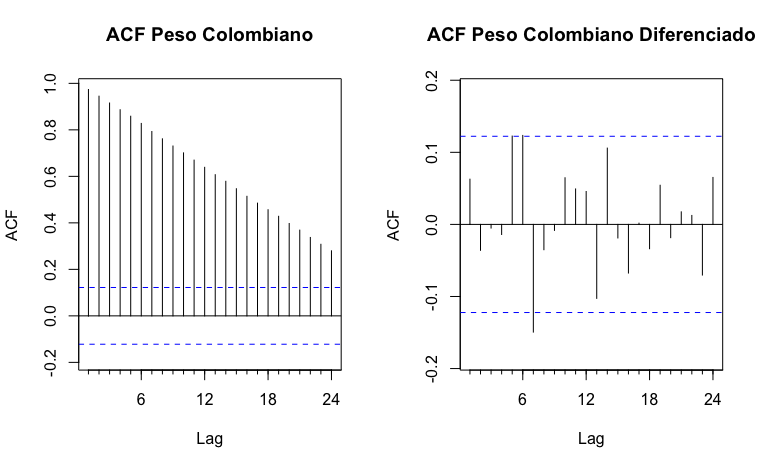
\includegraphics[width = 4 in]{DiffEjemploACF.png}
    \caption{Correlograma del Peso Colombiano Con y Sin Diferenciar (Fuente propia)}
\end{figure}

Una serie diferenciada es el cambio entre dos observaciones consecutivas y puede detallarse de la siguiente forma:

\[ y_{t}^{\prime} = y_{t} - y_{t-1} \]

Una serie diferenciada tendrá solo $T-1$ valores dado que no es posible calcular la diferencia $y_{1}^{\prime}$ para la primera observación. Cuando la serie diferenciada es ruido blanco, se la puede definir como:

\[ y_{t} = y_{t-1} - e_{t} \]

Las diferenciaciones también pueden hacerse por temporadas. Una diferenciación estacional es la diferencia entre una observación y su observación correspondiente del período pasado:

\[ y_{t}^{\prime} = y_{t} - y_{t-m} \]

donde $m$ es igual al número de temporadas. Estas se conocen como \emph{diferencias de m-retrasos}.

\subsubsection{Pruebas de Raíz Unitaria}
Una forma de determinar más objetivamente si hay necesidad de diferenciar una serie es la \emph{prueba de raíz unitaria}. Estas son pruebas de hipótesis estadísticas que están diseñadas para determinar la necesidad o no de diferenciación de la serie \cite{hyndman}. Existen varias y están basadas en diferentes enfoques, por lo que es común utilizar más de una si hay respuestas conflictivas que confrontar. 

La más utilizada es la prueba aumentada \emph{Dickey-Fuller}, también conocida como \emph{ADF}. Para este test, se utiliza el siguiente modelo de regresión \cite{dickeyfuller}:

\[ y_{t}^{\prime} = \phi y_{t-1} + \beta y_{t-1}^{\prime} + \beta_{2} y_{t-2}^{\prime} + \ldots + \beta_{k} y_{t-k}^{\prime} \]

donde $y_{t}^{\prime}$ denota la primera serie diferenciada, $y_{t}^{\prime} = y_{t} - y_{t-1}$ y $k$ es el número de retrasos para incluir en la regresión (que por regla común se ajusta a 3). Si la serie original, $y_{t}$, necesita diferenciarse, entonces el coeficiente $\hat{\phi}$ debiera aproximar a cero. Si $y_{t}$ ya es estacionaria, $\hat{\phi} < 0$. La metodología normal de test de hipótesis no funciona cuando la serie es estacionaria, pero el lenguaje \emph{R} tiene una función que lo calcula sin problemas de la forma \texttt{adf.test(x, alternative="stationary")} \cite{packageForecast}.

La hipótesis nula para una prueba \emph{Dickey-Fuller} es que la data es no-estacionaria. De tal manera que valores grandes de $p$ son indicativos de no-estacionalidad y valores pequeños de $p$ por el contrario indican que la hipótesis alternativa es de serie estacionaria. Un corolario de esto es que se necesita usar diferenciación cuando $p > 0.05$. 

\subsubsection{Modelos Autoregresivos (AR)}
En un modelo de regresión múltiple, pronosticamos la variable de interés usando una combinación lineal de predictores. En un modelo autoregresivo, el pronóstico de la variable de interés se conforma con una combinación lineal de valores pasados de la variable. El término autoregresión indica que es una regresión de variables contra si mismas \cite{hyndman}. 

Por lo tanto un modelo autogresivo de orden $p$ puede ser escrito como:

\[ y_{t} = c + \phi_{1}y_{t-1} + \phi_{2}y_{t-2} + \ldots + \phi_{p}y_{t-p} + e_{t}  \]

donde $e_{t}$ es ruido blanco. Es muy similar a la regresión múltiple pero con valores retrasados de $y_{t}$ como predictores. Esto se refiere a un modelo \textbf{AR(p)}. Los modelos autoregresivos son muy flexibles para manejar un portafolio amplio de patrones de series de datos. El cambio de los parámetros $\phi_1, \ldots, \phi_{p}$ resulta en diferentes patrones de series de datos. La varianza del término de error $e_t$ solo modifica la escala de la serie, no los patrones.

\subsubsection{Modelos de Promedios Móviles (MA)}
En vez de utilizar los valores pasados de una variable de pronóstico en una regresión, el modelo de promedios móviles utiliza los errores pasados del pronóstico en un modelo cuasi-regresión.

\[ y_{t} = c + e_{t} + \theta_{1}e_{t-1} + \theta_{2}e_{t-2} + \ldots + \theta_{q}e_{t-q} \]

donde $e_{t}$ es ruido blanco. Nos referimos a este modelo como \textbf{MA(q)}. En realidad no observamos los valores de $e_{t}$, por lo que no es una regresión en el sentido estricto de la palabra \cite{hyndman}. Hacemos notar que cada valor de $y_{t}$ puede ser pensado como un promedio móvil ponderado de los últimos errores de pronóstico. Sin embargo no hay que confundirlo con el suavizamiento de promedios móviles. El cambio de los parámetros $\phi_1, \ldots, \phi_{p}$ resulta en diferentes patrones de series de datos. Al igual que en los modelos autoregresivos, la variación del término de error $e_t$ solo modifica la escala de la serie, no los patrones.

\subsubsection{Modelos ARIMA No-Estacionarios}
Si combinamos la diferenciación con la autoregresión y un modelo de promedios móviles, obtenemos el \emph{modelo no-estacionario ARIMA}. ARIMA es el acrónimo para \emph{AutoRegressive Integrated Moving Average} (o modelos autoregresivos integrados de promedios móviles). En este caso son integrados porque la integración es la función opuesta de diferenciación \cite{hyndman}. Podemos escribir el modelo completo como:

\[ y_{t}^{\prime} = c + \phi_{1}y_{t-1}^{\prime} + \ldots + \phi_{p}y_{t-p}^{\prime} + \theta_{1}e_{t-1} + \ldots + \theta_{q}e_{t-q} + e_{t} \]

donde $y_{t}^{\prime}$ es la serie diferenciada (puede haber sido diferenciada más de una vez). Los predictores en la mano derecha de la ecuación incluyen tanto valores rezagados de $y_t$ y errores rezagados. A esto lo llamamos un modelo \textbf{ARIMA(p, d, q)}, donde:

\begin{description}
  \item [p = ]
  orden de la parte autoregresiva;
  \item [d = ]
  grado de la primera diferenciación involucrada; 
  \item [q = ]
  orden de la parte de promedios móviles.
\end{description}

Las mismas condiciones de estacionalidad e invertibilidad que se utiliza en los modelos de autoregresión y promedios móviles aplican al modelo ARIMA. 

\subsubsection{Gráficas ACF y PACF}
Seleccionar el juego indicado de variables \emph{p, d, q} puede ser difícil. Las bibliotecas de \emph{R} tienen funciones para ayudar. Por lo general no es posible a simple vista evaluar estos valores. Sin embargo, si es posible utilizar las gráficas de la función de autocorrelación ACF y su función asociada PACF para seleccionar valores de \textit{p} y \textit{q}. La gráfica de la función PACF mide la autocorrelación parcial entre $y_{t}$ y $y_{t-k}$ después de eliminar los efectos de otras series rezagadas $1, 2, 3, \ldots, k-1$. Por lo tanto la primer autocorrelación parcial es idéntica a la primer autocorrelación, porque no hay nada que eliminar. 

\begin{figure}[h!]
    \centering
    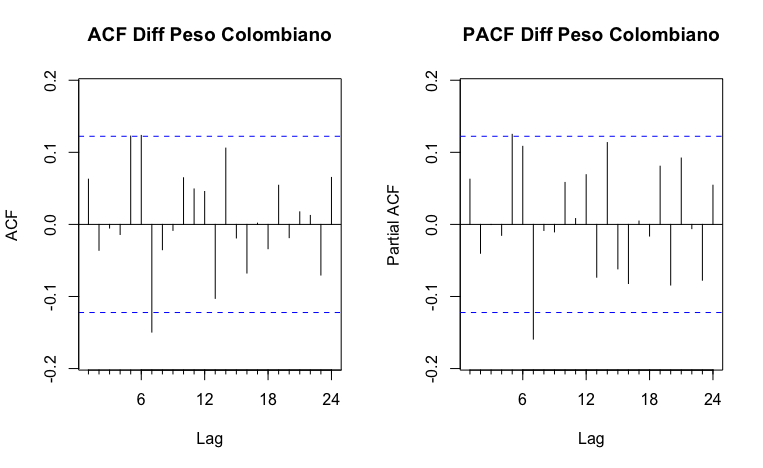
\includegraphics[width = 4 in]{ACFPACFEjemplo.png}
    \caption{Gráficas de las Funciones ACF y PACF del Peso Colombiano (Fuente propia)}
\end{figure}

Si los datos son de un modelo \textit{ARIMA(p,d,0)} o \textit{ARIMA (0,d,q)}, entonces las gráficas ACF y PACF pueden ser útiles en determinar los valores de \emph{p} o \emph{q}. Si tanto \emph{p} y \emph{q} son positivas, los gráficos no podrán ayudar a determinar los valores adecuados de \emph{p} y \emph{q}. 

Los datos pueden seguir un modelo ARIMA(p,d,0) si el gráfico ACF y PACF de los datos diferenciados muestran los siguientes patrones. 
\begin{itemize}
	\item La gráfica ACF decrece exponencialmente o tiene forma sinusoide 
	\item Hay un crecimiento significativo en el tramo \textit{p} en la gráfica PACF, pero ninguno después del tramo \textit{p}
\end{itemize}

Los datos pueden seguir un modelo ARIMA(0,d,q) si el gráfico ACF y PACF de los datos diferenciados muestran los siguientes patrones. 
\begin{itemize}
	\item La gráfica PACF decrece exponencialmente o tiene forma sinusoide 
	\item Hay un crecimiento significativo en el tramo \textit{p} en la gráfica ACF, pero ninguno después del tramo \textit{p}
\end{itemize}

\section{La Ciencia de Datos}
La Ciencia de Datos es una disciplina relativamente nueva, inclusive en muchos entornos académicos. El objetivo de este capítulo es el de resumir los aspectos mayores de la ciencia de datos como estudio multidisciplinario cuya intención es hacer sentido de la gran cantidad de datos que surgen de nuestro entorno, con miras a modificar los fenómenos del mundo.

\subsection{Introducción}
La ciencia de datos \cite{zumelMount} utiliza herramientas de otras ciencias empíricas, estadística, análisis matemático, finanzas, técnicas de visualización, inteligencia de negocios, sistemas expertos, aprendizaje automatizado, bases de datos, bioestadística, y ciencia de la computación con la finalidad de procesar y extraer conocimiento de la data, ya sea que esta se encuentre estructurada o no estructurada. 

Previo al termino Ciencia de Datos, el matemático John W. Tukey comienza a circular la idea del análisis de datos versus la estadística en su libro \textit{The Future of Data Analysis} \cite{tukey}. La premisa es que la estadística es una ciencia formal, mientras que el análisis de datos es una ciencia empírica ya que se basa en datos extraídos de la vida real. Tukey sostuvo que de la data debía extraerse hipótesis para evaluación, y que el análisis confirmatorio de datos debía coexistir al lado del análisis exploratorio de datos. Ambos se apoyan en la estadística como disciplina de aplicación pero estudian objetos diferentes. 

La ciencia de datos \cite{wikipediaDS} ha resultado para muchos una disciplina de reciente creación, pero en la realidad este concepto lo utilizó por primera vez el científico danés Peter Naur en la década de los sesenta como sustituto de las ciencias computacionales. En 1974 publicó el libro Concise Survey of Computer Methods 3 donde utiliza ampliamente el concepto ciencia de datos, lo que permitió que se comenzara a utilizar más libremente entre el mundo académico \cite{naur}.  

Por otro lado, el matemático japones e inventor de la \textit{Metodología de Cuantificación} Chikio Hayashi define sucintamente \cite{hayashi} la ciencia de datos no solo como un concepto sintético para unificar las disciplinas de la estadística, el análisis de datos, y sus métodos relacionados, sino por la forma en la cual sus resultados se aplican. Esta nueva metodología incluye tres fases: diseño de la data, recolección de la data, y análisis de la misma. 

Muchas veces se ha criticado a la ciencia de datos como el uso disimulado de estadística bajo un nombre diferente con fines comerciales. En 2001, William S. Cleveland introdujo a la ciencia de datos como una disciplina independiente, extendiendo el campo de la estadística para incluir los avances en computación con datos en su artículo \textit{Ciencia de datos: un plan de acción para expandir las áreas técnicas del campo de la estadística}. Cleveland estableció seis áreas técnicas que en su opinión conformarían al campo de la ciencia de datos: investigaciones multidisciplinarias, modelos y métodos para datos, computación con datos, pedagogía, evaluación de herramientas, y teoría \cite{cleveland}.

En abril del 2002, el \textit{ Council for Science: Committee on Data for Science and Technology} \cite{CODATA} empezó la publicación del \textit{Data Science Journal}, enfocada en problemas como la descripción de sistemas de datos, su publicación en Internet, sus aplicaciones y problemas legales. Poco después, en enero del 2003, la Universidad de Columbia empezó a publicar \textit{The Journal of Data Science}, la cual ofreció una plataforma para que todos los profesionales de datos presentaran sus perspectivas e intercambiaran ideas \cite{wikipediaDS}.

\subsection{El Científico de Datos y su Rol como Investigador}
Las personas que se dedican a la ciencia de datos se les conoce como científico de datos. El proyecto \textit{Master in Data Science} define al científico de datos como una mezcla de estadísticos, computólogos y pensadores creativos, con las siguientes habilidades:

\begin{itemize}
	\item Recopilar, procesar y extraer valor de las diversas y extensas bases de datos.
	\item Imaginación para comprender, visualizar y comunicar sus conclusiones a los no científicos de datos.
	\item Capacidad para crear soluciones basadas en datos que aumentan los beneficios, reducen los costos.
\end{itemize}

Los científicos de datos trabajan en todas las industrias y hacen frente a los grandes proyectos de datos en todos los niveles. La definición mas famosa de las habilidades que componen a un científico de datos se han atribuido al Dr. Nathan Yau \cite{yau}, quien precisó lo siguiente: \begin{quote} "... El científico de datos es un estadístico que debería aprender interfaces de programación de aplicaciones (API), bases de datos y extracción de datos; es un diseñador que deberá aprender a programar; y es un computólogo que deberá saber analizar y encontrar datos con significado." \end{quote}

En la tesis doctoral de Benjamin Fry \cite{fry} explicó que el proceso para comprender mejor a los datos comenzaba con una serie de números y el objetivo de responder preguntas sobre los datos, en cada fase del proceso que él propone (adquirir, analizar, filtrar, extraer, representar, refinar e interactuar), se requiere de diferentes enfoques especializados que aporten a una mejor comprensión de los datos. Entre los enfoques que menciona Fry están: ingenieros en sistemas, matemáticos, estadísticos, diseñadores gráficos, especialistas en visualización de la información y especialistas en interacciones hombre-máquina, mejor conocidos por sus siglas en inglés “HCI” (Human-Computer Interaction). Además, Fry afirmó que contar con diferentes enfoques especializados lejos de resolver el problema de entendimiento de datos, se convierte en parte del problema, ya que cada especialización conduce de manera aislada el problema y el camino hacia la solución se puede perder algo en cada transición del proceso.

\subsection{La Ciencia de Datos como Herramienta Predictiva}
Uno de los enfoques principales de la ciencia de datos es el procesamiento de datos estructurados o no estructurados para la obtención de conocimiento. Es importante destacar que la ciencia de datos trabaja en condiciones especiales que la definen de otras disciplinas (como por ejemplo, la inteligencia de negocios). 

\begin{itemize}
	\item Trabaja en datos incompletos; es muy probable que hasta un setenta por ciento del tiempo de un científico de datos se utilice en recopilar y curar datos aparentemente no-relacionados, incompletos, o altamente dispersos. 
	\item Los datos suelen estar desordenados; las fuentes de los datos a utilizar pueden ser de fuentes diversas y formatos diferentes, especialmente si estos datos provienen del Internet
	\item Analiza los datos para ver qué información obtiene; la exploración de datos no tiene garantía de hallazgo alguno como procedimiento científico, a diferencia de la inteligencia de negocios que opera sobre juegos de datos donde siempre hay certeza de al menos una conclusión 
	\item Los hallazgos impulsan decisiones sobre operaciones y productos; no solo de negocios sino dentro del mundo de la investigación de otras disciplinas, tales como la genética, biología, inteligencia artificial, etc.
\end{itemize}

Lo que distingue a la ciencia de datos de sus mismas técnicas y metodologías es su objetivo central de desplegar modelos efectivos para la toma de decisiones en un medio ambiente de producción. Así es una disciplina que que administra el proceso de transformar hipótesis y data en predicciones accionables \cite{zumelMount}. Los objetivos de predicción mas comunes incluyen la predicción de quien ganara una elección política presidencial, que productos se venderán mejor juntos, que créditos resultaran en moratoria, y cual pagina web el consumidor hará clic en la próxima hora. 

\subsection{Diseño de un Estudio de Ciencia de Datos}
El científico de datos es responsable de guiar el proyecto de ciencia de datos de comienzo a fin. El éxito de un proyecto de ciencia de datos no se da por la utilización de alguna herramienta en particular, sino de tener goles cuantificables, buena metodología, interacción interdisciplinaria, y un flujo de trabajo adecuado. Hay seis pasos principales en el diseño de un proyecto de ciencia de datos \cite{zumelMount}.

\begin{enumerate}
	\item \textbf{Definir el objetivo:} El primer paso en un proyecto de ciencia de datos es definir un objetivo medible y cuantificable. En esta etapa se trata de aprender todo lo posible sobre el contexto del problema. Un objetivo concreto incluye condiciones firmes para definir el éxito de la solución y criterios de aplicación.  
	\item \textbf{Recopilar y administrar la data:} El segundo paso incluye identificar los datos necesarios para alcanzar los objetivos propuestos, explorar dicha data, y acondicionarla para hacerla aplicable al análisis. Esta etapa suele ser una de las más intensiva en el uso de tiempo y recursos y es también la más importante. El investigador debe contestar las preguntas más críticas. ¿Qué datos se tienen disponibles? ¿Cuáles de estos datos son los necesarios para resolver el problema? ¿La data disponible es suficiente o se necesita más información? ¿La calidad de la data es óptima?
	\item \textbf{Construir el modelo de predicción:} La etapa de construcción del modelo es aquella donde se extrae información relevante de los datos para alcanzar el objetivo de estudio. Dado que muchas de las técnicas y procedimientos de modelos hace uso de suposiciones iniciales sobre la distribución de la data y sus relaciones, es muy probable que el investigador tenga que retroceder a la fase anterior, curar la data, y volver a la etapa de modelo en varias interacciones. 
	\item \textbf{Evaluar y criticar el modelo:} Una vez se obtiene el modelo, es necesario ver si se ajusta al problema en cuestión. ¿Es lo suficientemente preciso? ¿Su uso se generaliza bien? ¿Su desempeño es mejor que las herramientas disponibles existentes? ¿Los resultados del modelo (coeficientes, agrupaciones, reglas, etc.) hacen sentido dentro del contexto del problema?    
	\item \textbf{Presentar los hallazgos y documentar:} A partir del momento que el investigador aprueba el modelo de datos, es importante la presentación de los mismos con el rigor científico esperado por aquellos que tienen implicación o serán evaluadores del proyecto de investigación. 
	\item \textbf{Implementar el modelo en producción:} Muchos de los modelos de datos utilizados en la ciencia de datos deberán ser implementados como herramientas en la vida real. A esto se le conoce como despliegue en producción y tiene implicaciones de implementación que muchas veces salen de las manos del científico de datos y hacia el equipo de ingeniería. 
\end{enumerate}

Los renombrados científicos de Johns Hopkins University Roger Peng y Elizabeth Matsui prefieren hablar de epiciclos en su libro \emph{"The Art of Data Science"}. Un epiciclo se define como un un proceso iterativo que se aplica a todos los pasos del análisis de data. El epiciclo del análisis de datos incluye cinco pasos \cite{pengMatsui}.

\begin{enumerate}
	\item Formular y refinar la pregunta
	\item Explorar la data
	\item Construcción formal del modelo estadístico
	\item Interpretación de los resultados
	\item Comunicación de los resultados
\end{enumerate}

Estas cinco actividades pueden ocurrir en diferentes escalas de tiempo, con proyectos pequeños ejecutados en un día, y empréstitos mayores ocupando meses del tiempo de un equipo completo. Cada una de las cinco actividades del epiciclo a su vez se materializa a través de tres componentes principales.

\begin{enumerate}
	\item Establecer expectativas
	\item Recolección de datos, comparación con las expectativas, y resolución de conflictos cuando los datos y las expectativas no concuerdan
	\item Revisión de las expectativas, o los datos, según sea la prognosis del científico de datos
\end{enumerate}

La iteración de los tres pasos es lo que se denomina el \emph{epiciclo del análisis de datos} \cite{pengMatsui}. A medida que se avanza por cada una de las cinco fases del análisis, sera obligatorio iterar a través del epiciclo de análisis de datos para refinar la pregunta, la exploración inicial de datos, la interpretación y comunicación de los resultados. La siguiente tabla profundiza el uso de los tres pasos iterativos a través de dichas cinco fases. 

\begin{figure}[h!]
	\centering
	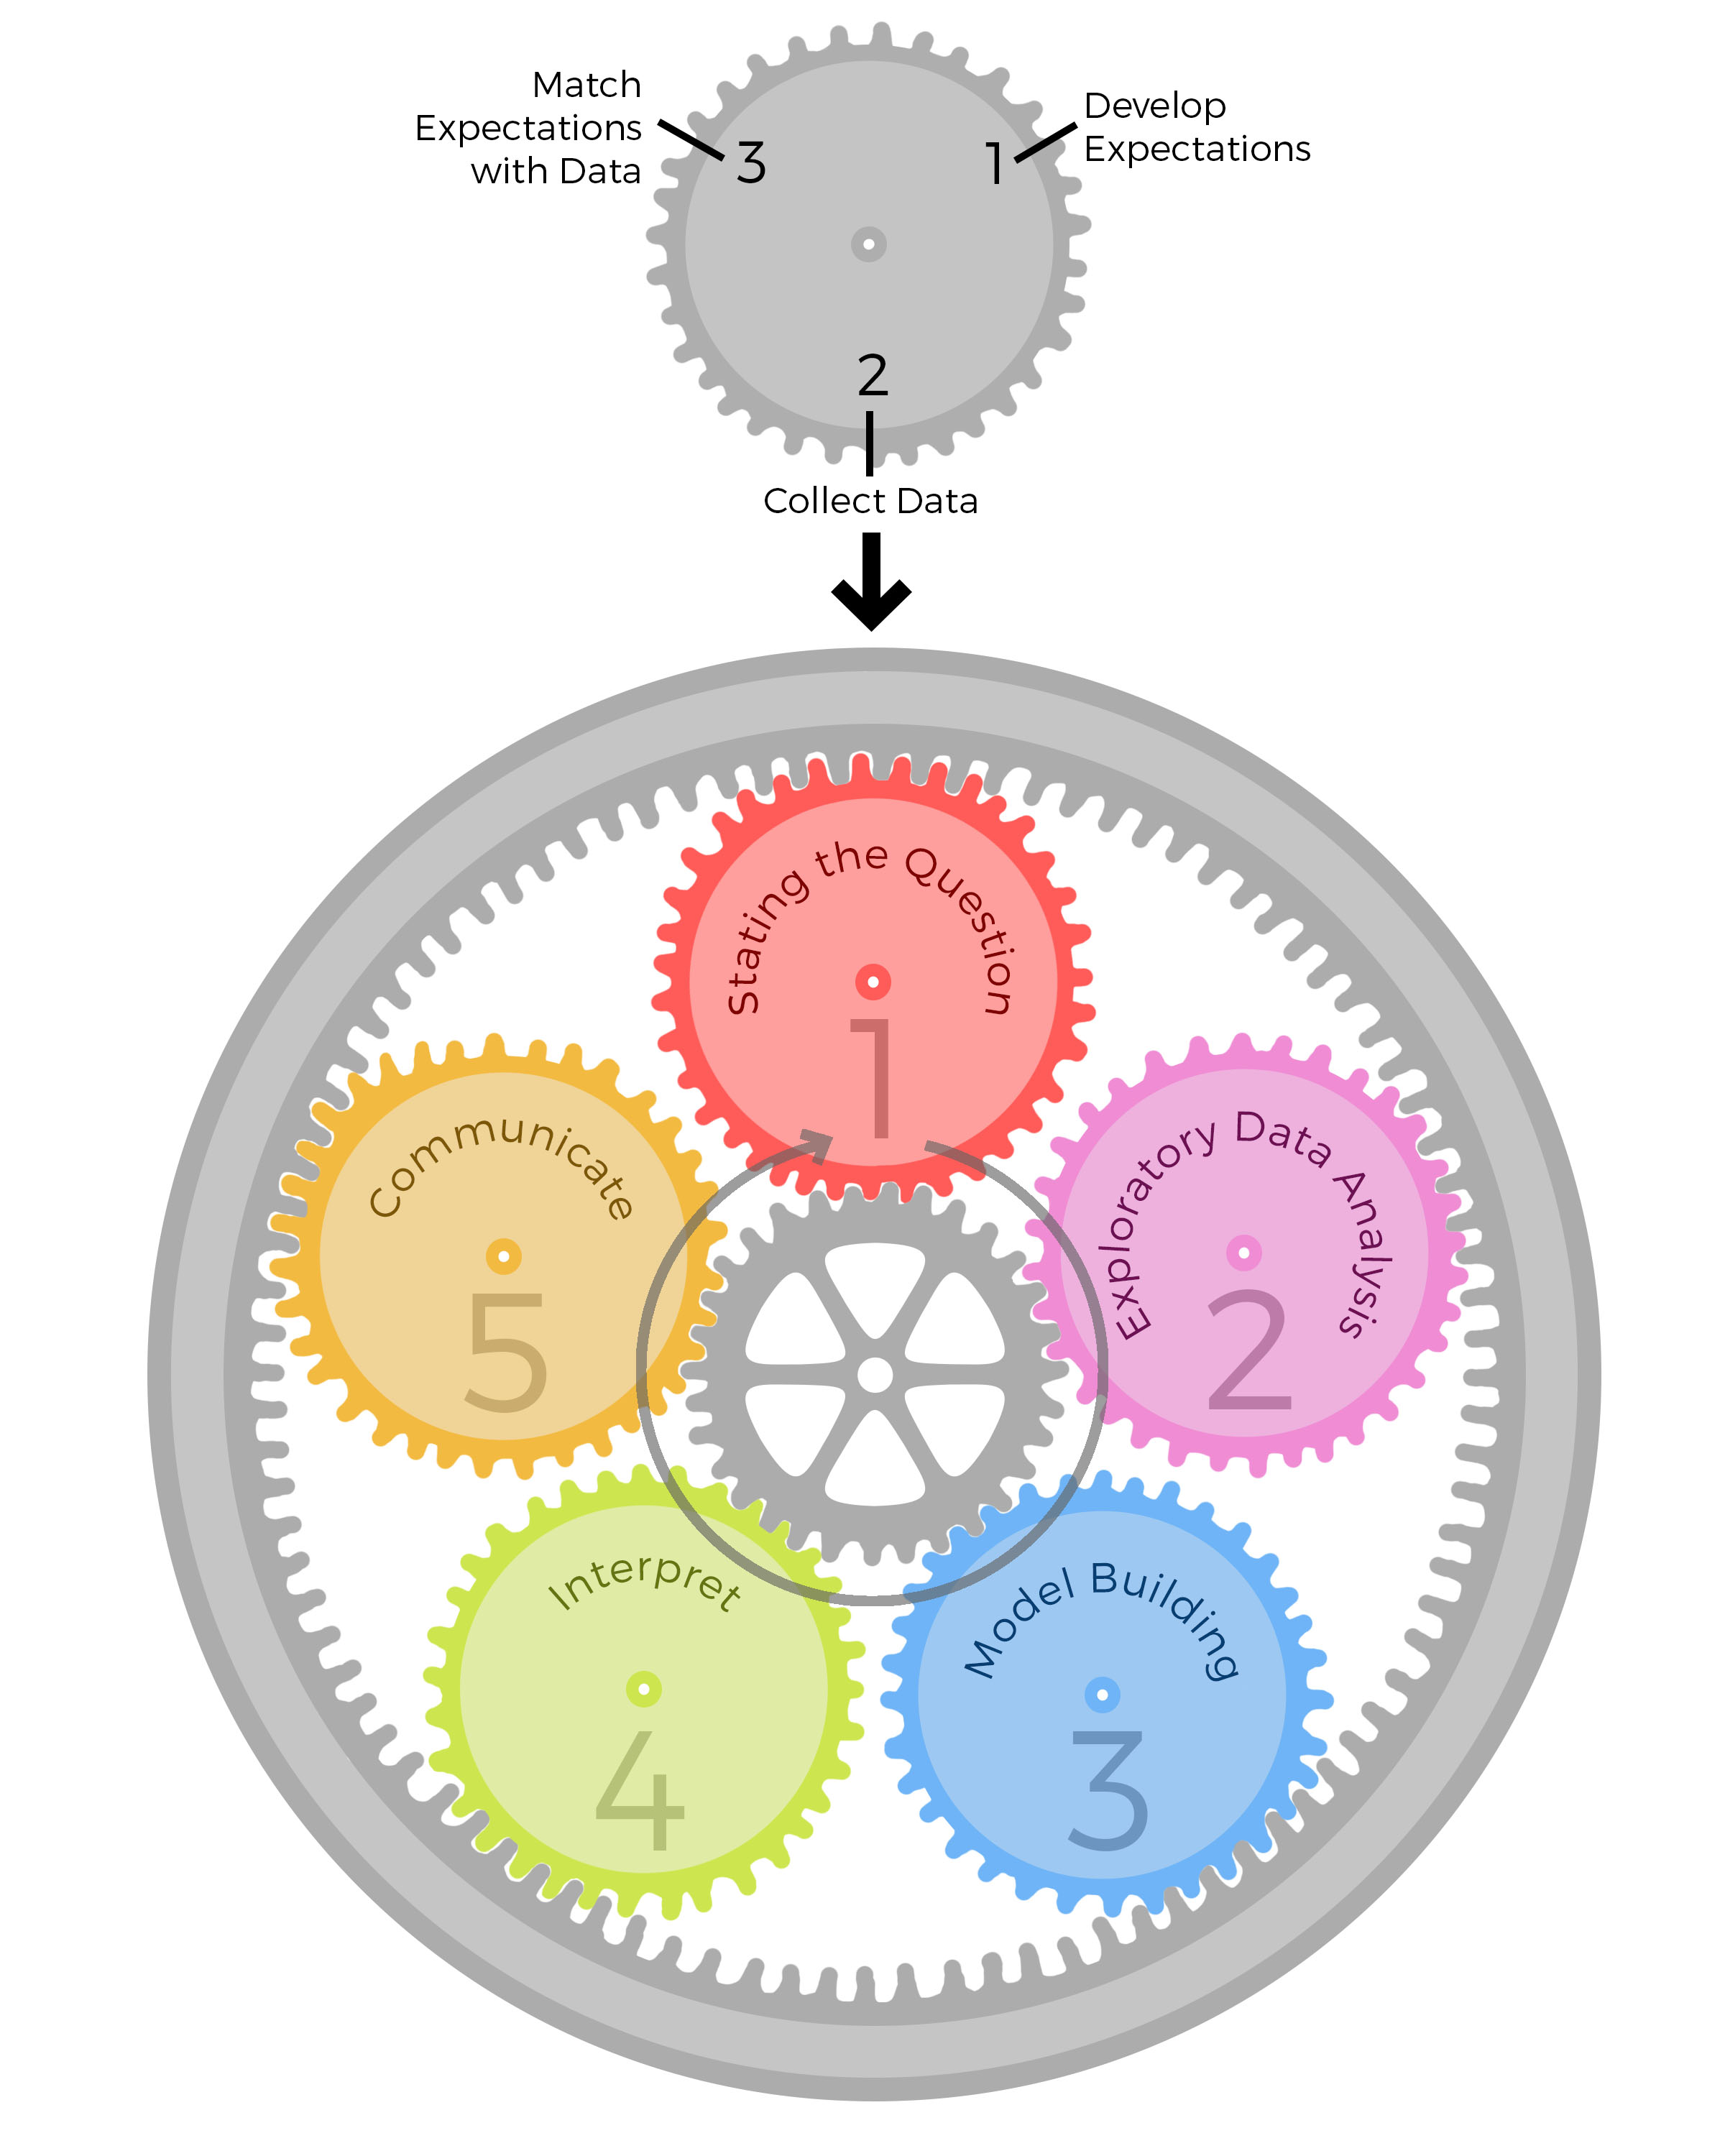
\includegraphics[width = 3in]{epicycle.png}
	\caption{Modelo de Epiciclos de Análisis de Datos (Fuente Peng y Matsui, 2017)}
\end{figure}

\subsection{Tareas Comunes en la Ciencia de Datos}
Hemos hablado de la ciencia de datos y su carácter predictivo. Las tareas mas comunes para lo cual se utiliza la ciencia de datos son las siguientes.

\begin{itemize}
	\item \textbf{Clasificación:} Decidir si algo pertenece a una categoría u otra. Harrington define la clasificación como la tarea de predecir a que tipo de clase pertenece una instancia (ejemplo) de la data propia de los métodos supervisados \cite{harrington}.
	\item \textbf{Puntuación:} Predecir o estimar un valor numérico, tal como lo es un precio o la probabilidad de un fenómeno. Alpaydin define esto como la extracción de reglas de los datos de los cuales se puede esperar estadísticamente un comportamiento similar y por lo cual se pueden efectuar predicciones correctas para instancias nuevas \cite{alpaydin}.
	\item \textbf{Ranking:} Aprender a ordenar objetos por preferencias
	\item \textbf{Agrupamientos:} Agrupar objetos en grupos de características homogéneas. Las técnicas de agrupamiento son típicas de los métodos de aprendizaje automatizado no-supervisados, donde en vez de buscar clasificar en clases conocidas o puntuar con valores ciertos, se busca la características comunes de la data para la agrupación de la misma en clases, tomando en cuenta que dichas clases no son conocidas a priori \cite{harrington}. 
	\item \textbf{Relaciones:} Encontrar relaciones o causas potenciales de efecto tal cual se ven en la data. Para Alpaydin la regresión lineal es un perfecto ejemplo de búsqueda de relaciones en la ciencia de datos, donde existe una función con un juego de parámetros asociados $y = g(x \mid \theta)$, $g(.)$ es el modelo y $\theta$ son sus parámetros. $Y$ es un número dentro de una regresión y $g(.)$ es la función de la regresión \cite{alpaydin}
	\item \textbf{Caracterizaciones:} Utilización general de visualizaciones y reportes de la data. Un ejemplo notable lo da Witten y Frank al referirse a la técnica de \emph{Market Basket Analysis} dentro de la mercadotecnia \cite{datamining}. En dicha técnica se busca que otros artículos comprarán los consumidores basados en el comportamiento registrado de sus compras pasadas. En términos matemáticos, estamos buscando $P(Y \mid X,D) = x_i$ donde $D$ es el juego conocido de datos históricos de los movimientos comerciales de los consumidores. 
\end{itemize}

\pagebreak
\section{Aprendizaje Automatizado}
El aprendizaje automatizado es un campo de la ciencia de la computación donde se busca darle a las computadores la habilidad de aprender sin ser explicitamente programadas. El término se le atribuye a \textbf{Arthur Samuel}, un pionero del campo de la inteligencia artificial, quien lo acuñó en 1959 (Kohavi, R. y Provost, F., 1998).

Es interesante que los métodos de aprendizaje automatizado proliferaron de forma paralela al concepto de ciencia de datos, y solo fueron absorbidos por esta en los últimos diez años. Alpaydim nos describe el aprendizaje automatizado como la programación de computadoras para optimizar un criterio de desempeño utilizando datos o experiencia pasada (Alpaydim, E., 2010). Tom Mitchell respeta este concepto al describir el aprendizaje automatizado como "\ldots la construcción de programas computacionales que aprenden con la experiencia\ldots” (Mitchell, T., 1997, pág. XV). Solo Peter Harrington utiliza una descripción mucho más simplista al determinar que “El aprendizaje automatizado es la extracción de información de la data.” (Harrington, P. 2012, pág. 5).

Estudiar los procedimientos de aprendizaje automatizado equivale a estudiar tres temas principales que los componen.

\begin{itemize}
	\item Diseño del estudio: conjuntos de entrenamiento y conjuntos de predicción
	\item Problemas conceptuales: error fuera de la muestra, curvas ROC
	\item Implementación práctica: en este caso en particular, un tema que se cubrirá con la biblioteca Caret
\end{itemize}

Todo el mundo predice todo tipo de aseveraciones, desde el resultado de una elección presidencial hasta el partido de fútbol del domingo de una liga en particular. Pero en el sentido estricto de la palabra, ¿qué significa predecir? En nuestro contexto científico, definiremos el acto de predecir como el resultado de utilizar la probabilidad y muestreo para la selección de un conjunto de entrenamiento, el cual utilizaremos para construir las características de diseño de una función de predicción. La función utilizará dichas características para generar nuevas predicciones.  Los componentes para la selección adecuada de variables de predicción son los siguientes:

TO DO: Agregar el siguiente esquema
Pregunta > Datos > Atributos > Algoritmo > Parámetros > Evaluación

Un ejemplo muy común utilizado generalmente para explicar el uso del aprendizaje automatizado es la detección de correo chatarra, también conocido como spam. Podemos utilizar atributos cuantitativos de los mensajes, por ejemplo la frecuencia de ciertas palabras, para que un modelo se entrene y pueda predecir dentro de ciertos rangos de certeza si un correo cualquiera es o no spam.

\subsection{Importancia Relativa de Los Pasos}

Hay una secuencia de pasos importante para la consecución de modelos de aprendizaje automatizado coherentes.

TO DO: Agregar el siguiente esquema como gráfico
Pregunta : Data : Atributos : Algoritmos

La combinación de algunos datos y un deseo extremo de conseguir una respuesta no nos asegura que una razonable pueda extraerse de un cuerpo cualquiera de información (Tukey, 1977). También es útil recordar que la calidad de los datos que ingresan al conjunto de entrenamiento tienen un efecto sobre el resultado del modelo. Datos que no son útiles no aportan nada. Es mucho mejor que la data sea curada y organizada de manera que tenga alta relevancia al tema de estudio.

Los buenos atributos son aquellos que comparten las siguientes características:

\begin{enumerate}
	\item ayudan a comprimir la data
	\item retienen el mayor volumen de información relevante
	\item son creados basados en un modelo experto del modelo a aplicarse
\end{enumerate}

No es fácil hacer una buena selección de atributos que mas adelante se convertirán en variables de predicción. Los errores mas comunes son los siguientes.

\begin{enumerate}
	\item tratar de automatizar la selección de atributos
	\item no prestar la atención necesaria a las variaciones y particularidades de los datos
	\item desechar información importante innecesariamente
\end{enumerate}

En este sentido los algoritmos importan mucho menos que la selección y curación de la data a utilizar. Los mejores métodos de aprendizaje automatizado reúnen una serie de características que los hace justamente sobresalir del montón. Las características en mención son las siguientes:

\begin{enumerate}
	\item Interpretable:
	\item Simples:
	\item Precisos:
	\item Rápidos (de entrenar y evaluar):
	\item Escalables:
\end{enumerate}

La predicción de modelos se basa mucho en el arte de compensar beneficios versus necesidades.

\begin{enumerate}
	\item interpretación de los datos vs. precisión
	\item velocidad vs. precisión
	\item simplicidad vs. precisión
	\item modelos escalables vs. precisión
\end{enumerate}

A pesar de tener que sopesar la mejor forma de compensar todas estas variables, la interpretación es muy importante y debe conservar su lugar, ya que poco sirve un modelo rápido y preciso que no se puede interpretar. Muchos autores otorgan un segundo lugar de importancia a lo escalable del modelo. Se han dado casos donde modelos muy precisos no se han podido poner en producción por la complejidad de escalar el algoritmo. El caso mas mencionado es el premio NETFLIX, el cual otorgo un millón de dolares al equipo con el mejor modelo de predicción de gustos de sus clientes, solo para luego llegar a la conclusión que el mismo era demasiado complejo y lento de escalar en producción y archivarlo (Techdirt, 2012).

\subsection{Métodos Supervisados y No-Supervisados}
Para los autores Hastie, Tibshirani, y Friedman el aprendizaje supervisado intenta aprender una función f de predicción a través del uso de uso juegos de datos de entrenamiento en forma de muestras del total de los datos disponibles. El uso de datos de entrenamiento le permite al sistema aprender y minimizar el error del modelo de predicción \cite{theElements}.

Harrington nos da una explicación más sencilla del término, al aclarar que el aprendizaje supervisado es aquel que le pide al computador aprender de los datos utilizando una variable específica como objetivo. Esto reduce la complejidad de algoritmos y patrones que se deben derivar de la muestra de datos \cite{harrington}.

El profesor Alpaydin agrega que el aprendizaje supervisado tiene como objeto aprender un mapeo de los elementos de entrada a los de salida, teniendo en cuenta que los valores correctos de estos últimos están dados por el supervisor \cite{alpaydin}.

\subsection{Error Muestral y Error Fuera de Muestra}
El siguiente concepto es fundamental dentro de la teoría de aprendizaje automatizado, y la terminología puede diferir un poco de los términos establecidos en la estadística inferencial.

	\begin{itemize}
		\item \textbf{Error dentro de la muestra:} es el margen de error que se obtiene al utilizar el juego de datos de entrenamiento en la construcción del modelo de predicción. También se conoce como error de re-substitución
		\item  \textbf{Error fuera de muestra:} es el margen de error que se obtiene cuando se aplica el modelo de predicción a un nuevo juego de datos. También se lo conoce como error de generalización.
	\end{itemize}


En este punto debemos aclarar cuales son las ideas principales en las que hay que enfocarse.

\begin{enumerate}
	\item Principalmente estamos interesados mucho mas en el error de generalización - el que se obtiene al aplicar un nuevo juego de datos al modelo de predicción - que del margen de error de resubstitución.
	\item El error de resubstitución siempre va a ser menor que el error de generalización
	\item La razon por la cual se da este fenómeno (que el error de resubstitución sea menor que el error de generalización) es el efecto de sobreajuste. El algoritmo se está ajustando de más a los datos.
\end{enumerate}

La data en la ciencia de datos tiene dos partes: señal y ruido. El objetivo del modelo de predicción es el de predecir la señal. Siempre se puede diseñar un modelo perfecto que capture tanto la señal como el ruido. Pero dicho modelo no se desempeñará bien en juegos de datos nuevos.

El efecto de sobreajuste se como la creación de un modelo optimista a partir del juego de datos de entrenamiento. Los métodos que utilizamos buscan interpretar los datos de tal manera que no solo se ajustan a la señal sino al ruido de los mismos. Por esa razón el margen de error de resubstitución (error dentro de la muestra) es tan bajo pero cuando se prueba el mismo modelo entrenado en un juego de datos externo el margen de error generalizado (fuera de la muestra) crece. Se ha comprobado que los errores por sobreajuste ocurren más en modelos complejos que en modelos sencillos. La razón es que muchas veces el modelo complejo es precisamente más complicado para ajustarse mejor a la señal de los datos, sin que estos ajustes sean necesarios - o precisos - al momento de cambiar del juego de datos.

\subsection{Diseño de un Estudio de Aprendizaje Automatizado}
El diseño de una investigación de ciencia de datos tiene seis pasos. El diseño del estudio de un problema de aprendizaje automatizado debe verse como el diseño de la fase de modelo (paso tres) mucho más detallado para no confundirlos. La metodología recomendada por el Dr. Jeff Leek (Leek, J. 2015) recomienda los siguientes seis:

\begin{enumerate}
	\item Definir el margen de error deseado
	\item Dividir la data en juegos específicos de entrenamiento, evaluación y validación (opcional)
	\item En el juego de entrenamiento, seleccionar atributos y utilizar validación cruzada
	\item En el juego de entrenamiento, seleccionar la función de predicción; utilizar nuevamente validación cruzada
	\item si no se utilizo validación cruzada, aplicar prueba 1X al juego de evaluación
	\item si se utilizo validación cruzada, aplicar prueba al juego de evaluación, refinar el algoritmo, y luego volver a someter 1X al juego de validación
\end{enumerate}

A pesar de que no tiene una comprobación científica, la comunidad siempre aconseja evitar las muestras pequeñas de la misma forma que se evitan en la estadística clásica. Una pregunta válida es cuanto de los datos disponibles se deben destinar al juego de entrenamiento, cuantos al juego de validación y cuantos al juego de evaluación. Zumel y Mount (Zumel, N., Mount, J., 2014) consideran un modelo sencillo de división con 90\% de los datos destinados al entrenamiento de modelos y el 10\% restante a la evaluación. Sin embargo Leek (Leek, J. 2015) en su libro \emph{Data Style} nos da un juego de reglas mas comprensivas de como distribuir los datos segun el volumen de los mismos.

\textbf{A. Si el volumen de datos es grande}
\begin{itemize}
	\item 60\% para el juego de entrenamiento
	\item 20\% para el juego de evaluación
	\item 20\% para el juego de validación
\end{itemize}

\textbf{B. Si el volumen de datos es mediano}
\begin{itemize}
	\item 60\% para el juego de entrenamiento
	\item 40\% para el juego de evaluación
\end{itemize}

\textbf{C. Si el volumen de datos es pequeño}
\begin{itemize}
	\item entrenar sobre el 100\% de los datos
	\item utilizar validación cruzada sobre el mismo juego que se entrenó
	\item no ocultar el hecho hacer alusión en la investigación de la muestra poco representativa
\end{itemize}

La tentación de utilizar el juego de datos de validación y/o evaluación es muy grande para todos los científicos de datos noveles. Sin embargo la literatura concuerda en que no se debe utilizar la evaluación sino hacia el final del proceso.

La selección de que datos en particular deben elegirse en cada grupo debe ser aleatoria, con un porcentaje definido en cada uno pero total certeza de que no hay parcialidad en la selección. En el caso del lenguaje R, la biblioteca CARET tiene incorporada funciones para garantizar asignaciones de datos a los grupos de entrenamiento y evaluación totalmente aleatorios. Los juegos finales de datos deben reflejar sin embargo las mismas estructuras del problema. Un claro ejemplo son las series de tiempo (Hyndman, R., 2012) en las cuales los datos tiene un componente de tiempo que denota un orden en especial. De estos grupos debe seleccionarse muestras aleatorias pero representativas de los periodos de tiempo a fin de tener sentido. A su vez cada sub-muestra debe reflejar el mayor grado de diversidad posible. Esto se debe lograr con selección aleatoria pero a veces es difícil mantener dicho balance con la mezcla posible de atributos.

\subsection{Tipo de Errores}
El concepto de error en estadística es uno que embarca varias dimensiones. En lo que respecta al aprendizaje automatizado, no importa que tan grande sea la muestra ni que tan exacto sea el algoritmo, siempre cabe la probabilidad - aunque pequeña - que una predicción sea falsa a pesar de que arroja un resultado positivo. Podemos entonces dividir los tipos de errores según su predicción y verdadera naturaleza (Yakir, B. 2011).

En lineas generales diremos que un resultado es positivo si ha sido identificado como tal, y que es negativo si ha sido rechazado. De tal forma:
\begin{itemize}
	\item \textbf{verdadero positivo:} es aquel que ha sido correctamente identificado
	\item \textbf{falso positivo:} es aquel que ha sido incorrectamente identificado
	\item \textbf{verdadero negativo:} es aquel que ha sido correctamente rechazado
	\item \textbf{falso negativo:} es aquel que ha sido incorrectamente rechazado
\end{itemize}

La combinación de los siguientes resultados nos permite medir estadísticamente variables pertinentes a los resultados del modelo. Estas variables se conocen como sensibilidad, especificidad, valor predictivo positivo, valor predictivo negativo, y exactitud.

\textbf{Sensibilidad:} La sensibilidad es la probabilidad que un fenómeno arroje un valor positivo cuando realmente lo es. Por ejemplo, un examen de una enfermedad da positivo cuando el paciente realmente esta enfermo de dicho padecer. Podemos expresar la formula como un cociente de la siguiente forma:

\begin{equation}
sensibilidad = \frac{VP}{(VP + FN)}
\end{equation}

\textbf{Especificidad:} La especificidad es la probabilidad que un fenómeno arroje un valor negativo cuando realmente no se encuentra presente (o sea es una predicción negativa cuando la realidad también es negativo). Por ejemplo, un examen de embarazo que da negativo cuando la paciente no esta embarazada. Podemos expresar la formula como un cociente de la siguiente forma:

\begin{equation}
especificidad= \frac{VN}{(FP + VN)}
\end{equation}

\textbf{Valor Predictivo Positivo:} El valor predictivo positivo es la probabilidad de que un fenomeno este presente cuando la predicción arroja un valor positivo. Por ejemplo, la probabilidad de que un paciente tenga diabetes cuando el examen arroja positivo. Podemos expresar la formula como un cociente de la siguiente forma:

\begin{equation}
\mbox{\textit{valor predictivo positivo}} = \frac{VP}{(VP + FP)}
\end{equation}

\textbf{Valor Predictivo Negativo:} Lo opuesto del valor predictivo positivo, es la probabilidad de que una prediccion arroje negativo cuando el fenómeno no este presente. Por ejemplo, la probabilidad de que un paciente no se le detecte diabetes cuando en la vida real no la tiene. Podemos expresar la formula como un cociente de la siguiente forma:

\begin{equation}
\mbox{\textit{valor predictivo negativo}} = \frac{VN}{(VN + FN)}
\end{equation}

\textbf{Exactitud:} Quizás el mas sencillo de percibir de forma natural, la exactitud es simplemente la probabilidad de una prediccion correcta. Podemos expresar la formula como un cociente de la siguiente forma:

\begin{equation}
exactitud = \frac{VP + VN}{(VP + FP + VN + FN)}
\end{equation}

\subsubsection{Midiendo Error en Data Continua}
Para data continua, de naturaleza numérico, las dos formas de medir el error mas comunes en aprendizaje automatizado son el error cuadrático medio y la raíz error cuadrático medio.

La raíz error cuadrático media es utilizada con frecuencia para medir la diferencia entre valores (de una muestra y valores de una población) predicha por un modelo o un estimador y los datos observados en la realidad. Este valor representa la desviación estándar de la muestra entre los valores predecidos y los valores observados. Las diferencias individuales entre estas dos medidas se conocen como residuos si son extraídos de la muestra, y errores de predicción si son calculados fuera de muestra.

\begin{equation}
\sqrt{\frac{1}{n}\sum_{i=1}^n(prediccion_{i} - observado_{i})^{2}}
\end{equation}

\subsection{Sobreajuste}
En aprendizaje automatizado, el sobreajuste (también es frecuente emplear el término en inglés overfitting) es el efecto de sobre-entrenar un algoritmo de aprendizaje con unos ciertos datos para los que se conoce el resultado deseado. Daroczi define el sobreajuste como la descripción del modelo en conjunto con el ruido aleatorio de la muestra en vez de solo el fenómeno generador de datos \cite{daroczi}. El sobreajuste ocurre, por ejemplo, cuando el modelo tiene más predictores de los que puede acomodar la muestra de datos.

Según Zumel y Mount, una de las señales de sobreajuste más sencillas de detectar se da cuando un modelo tiene un excelente desempeño en el juego de datos que se entrenó, pero uno muy malo en un juego de datos nuevo \cite{zumelMount}. Esto es causa y efecto de memorizar la data de entrenamiento en vez de aprender reglas generales de la generación del patrón.

\subsection{R y la Biblioteca CARET}
La biblioteca \emph{CARET} (nombre extraído de Classification And Regression Training) es una libreria de funciones en R para optimizar el proceso de crear modelos predictivos. El paquete contiene herramientas para:

\begin{itemize}
	\item segmentar juegos de datos
	\item preproceso de los datos
	\item seleccion de predictores
	\item optimizacion del modelo utilizando reconfiguracion de muestras
	\item estimacion de la importancia de la variable
\end{itemize}

El paquete esta mantenido en GitHub bajo la administración del Doctor en Estadística Max Kuhn.

\section{Modelos Ensamblados}
El tema de modelos ensamblados es uno que por lo general se reserva más como técnica de composición que cómo teoría del aprendizaje automatizado. Los modelos ensamblados ayudan a mejorar los resultados del aprendizaje automatizado combinando diferentes modelos. Este enfoque permite la producción de mejores modelos predictivos en contraposición a la utilización de un solo modelo \cite{smolyakov}.

\subsection{Introducción}
  El uso de modelos ensamblados es en cierta forma la prueba final de la hipótesis de trabajo: la utilización de dos modelos entrecruzados cuyos resultados conforman una tabla temporal de valores esperados de los cuales se genera un nuevo modelo sintético de predicción más general y con mayor capacidad de predicción en juegos de datos de validación cruzada. Este concepto es novel; Witten y Frank lo describen como combinación de métodos múltiples, y escriben: “… un enfoque obvio para hacer mejores decisiones es tomar el resultado de diferentes métodos y combinarlos\ldots” \cite{datamining}. Zhou nos describe que “… los modelos ensamblados que entrenan múltiples variables y luego las combinan para uso de entrenamiento, con el Boosting y el Bagging como representantes principales, representan lo más novedoso en el estado del arte de la ciencia de datos…” \cite[p. 7]{ensembleMethods}. De una manera un tanto más coloquial, Zhang y Ma describen el uso de modelos ensamblados con una analogía de la vida real, en la cual los pacientes buscan una segunda y hasta tercera opinión de expertos antes de someterse a una operación complicada \cite{ensembleMachineLearning}. Curiosamente tanto Zhang, Ma y Zhou hablan de la combinación de métodos de regresión general con clasificadores, y solo Witten y Frank hablan de otras combinaciones (por supuesto, Witten y Frank comenzaban a escribir en los albores del ensamblaje de métodos, cuando los clasificadores no estaban tan de moda porque el análisis era mayoritariamente de números, algo que cambió con el avance de las redes sociales). Una de las descripciones más sucintas y prácticas es la de Vadim Smolyakov, quien define el uso de modelos ensamblados como meta-algoritmos que combinan dos o más técnicas de aprendizaje automatizado en un modelo predictivo de forma que se logre disminuir la varianza (bagging), el sesgo (boosting) o se mejore la precisión (stacking) \cite{smolyakov}. 

\subsection{Combinando Métodos}
La combinación de métodos es el último paso en la estrategia de construcción de un sistema ensamblado de aprendizaje automatizado. La pregunta de que métodos combinar esta estrechamente relacionado con el tipo de juegos de datos y la solución que se busca alcanzar. Por ejemplo, alguno métodos de clasificación como los vectores de soporte solo devuelven valores discretos \cite{ensembleMachineLearning}. De tal manera el uso de dos métodos alternos en uno ensamblado estará determinado por la forma final en que se ensamblan y el algoritmo final utilizado para la decisión de predicción. Tanto Polikar \cite{ensembleMachineLearning} como Zhou \cite{ensembleMethods} citan como preferibles las metodologías de voto por mayoría, promedio, promedio ponderado, y ensamblaje infinito. Dzeroski y Zenko denotan que la mayoría de la investigación alrededor de métodos ensamblados se da con la generación de ensambles utilizando un único algoritmo de clasificación, como por ejemplo los árboles de decisión o el entrenamiento de redes neuronales \cite{DzeroskiZenko}. 

Smolyakov divide los métodos ensamblados en dos grandes clasificaciones \cite{smolyakov}:

\begin{itemize}
  \item \textbf{Métodos Ensamblados Secuenciales:} son aquellos donde los modelos bases de aprendizaje se generan de forma secuencial. La idea inicial es que se explota la dependencia entre dichos modelos base al momento de generarlos. Un buen ejemplo de modelos ensamblados secuenciales es \emph{AdaBoost}. El desempeño de predicción o la acotación del margen de error se optimiza al calibrar los regresores y/o clasificadores después de cada entrenamiento y previo al próximo. 
  \item \textbf{Métodos Ensamblados Paralelos:} son aquellos en los cuales los modelos bases se generar en forma paralela e independiente. Un buen ejemplo de modelos ensamblados paralelos es \emph{Random Forest}. La motivación de utilizar modelos ensamblados paralelos es maximizar la independencia entre los regresores y/o clasificadores que se optimizan entre si al promediar los resultados, reduciendo el margen de error. 
\end{itemize}

\subsection{Diversidad}
La diversidad de ensamblaje, o la diferencia entre diferentes métodos de aprendizaje, es un tema fundamental en el ensamblaje de métodos \cite{ensembleMethods}. Intuitivamente es fácil entender que para obtener una ventaja de la combinación, es necesario que los aprendizajes sean diferentes, de otra manera la ganancia en desempeño no seria marginalmente superior a los métodos por separado \cite{ensembleMethods}.

La mayoría de los métodos ensamblados utilizan solo un tipo de modelo base de algoritmo de aprendizaje para producir regresores o clasificadores homogéneos (del mismo tipo) conocidos como \textit{ensamblajes homogéneos} \cite{smolyakov}. También existen métodos que utilizan diferentes tipos de modelos bases como clasificadores y/o regresores. Estos modelos ensamblados se conocen como \textit{modelos heterogéneos}. Para poder ensamblar modelos más precisos que cualquiera de sus modelos base por si solos es necesario que los modelos bases sean precisos en primera instancia, y tan diversos como sea matemáticamente posible \cite{smolyakov}.

Para propósitos de este marco teórico revisaremos de forma breve los tres métodos más utilizados en la actualidad para el ensamblaje que son:
\begin{itemize}
  \item Bagging: cuando se busca reducir la varianza en los clasificadores
  \item Boosting: cuando se busca reducir el sesgo 
  \item Stacking: cuando se busca aumentar la predicción de los regresores
\end{itemize}

Dado que la hipótesis de trabajo del siguiente estudio utiliza el ensamblaje heterogéneo de modelos bases de regresión lineal y pronóstico de series de tiempo con ARIMA, haremos un alto para entrar con más detalle en la teoría y bondades de los modelos apilados (\emph{stacking}).

\subsection{Bagging}
La idea del \emph{bagging} esta estrechamente ligada al \emph{bootstrapping}, y determinada por la selección de múltiples muestras de datos generadas a través de \emph{bootstrapping}, utilizadas para alimentar clasificadores, sobre cuyos resultados el método ensamblado puede votar \cite{daume}. La palabra \emph{bagging} es la composición de \emph{bootstrap aggregation}. La etimología proviene de la metodología propia del método, que usa la agregación de múltiples muestras generadas de los datos disponibles (por ende, el \emph{bootstrapping}) para promediar múltiples estimados \cite{smolyakov}. 
Por ejemplo, se pudiera utilizar el \emph{bagging} para entrenar M árboles diferentes en diferentes juegos de datos seleccionados al azar con reemplazo para computar el ensamblado siguiente:  

\[ f(x) = \frac{1}{M} \sum_{m=1}^M f_m^{(x)} \]

\emph{Bagging} utiliza muestreo por \emph{bootstrap} para obtener juegos de datos para entrenar los modelos base. Para agregar los resultados de los modelos base, el \emph{bagging} utiliza dos maneras:
\begin{enumerate}
  \item Votación para clasificadores
  \item Promedios para regresión
\end{enumerate}

\subsection{Boosting}
El \emph{boosting} se refiere a una familia de técnicas de algoritmos que tienen la capacidad de convertir clasificadores (o regresores) débiles en entrenadores fuertes. El principio del \emph{boosting} es calzar una secuencia de clasificadores débiles - modelos que son escasamente mejores en la predicción que selección al azar, como por ejemplo pequeños árboles de decisión - a versiones ajustadas y sopesadas de los datos. Más peso se le otorga a los clasificadores que fueron mal clasificados en rondas anteriores \cite{smolyakov}. Daume describe el método como "\ldots La forma en la cual funciona el \emph{boosting} es que basado en un juego de datos y resultados pasados, va generando nuevas predicciones. Las predicciones con resultados aceptables se les pone menor peso y recursos, mientras que el algoritmo vuelve a iterar en aquellas predicciones con valores lejanos hasta que cobran fuerza \ldots" \cite{daume}. Esta técnica recibe el nombre de \textbf{AdaBoost}, del ingles \emph{adaptive boosting algotithm}. \textbf{AdaBoost} fue una de las primeras técnicas practicas en la ciencia de datos.

Los algoritmos de \emph{AdaBoost} comienzan ajustando los pesos del clasificador base \(y_1(x)\) a \(\frac{1}{N}\). Al comienzo todos los coeficientes de peso son los mismos. En rondas subsiguientes los coeficientes de peso se aumentan para aquellos puntos de datos que han sido mal clasificados y se reduce el peso de aquellos que han sido clasificados correctamente. Esta iteración es la que permite fortalecer los clasificadores débiles (a la vez fortaleciendo los débiles y debilitando los fuertes para contrastar mejor) \cite{smolyakov}. 

Existe una variable epsilon que representa el error ajustado de cada clasificador base. Hacia el final de las iteraciones del algoritmo los coeficientes ajustados alfa le otorgan mayor peso a los clasificadores con mayor precisión (la cual ha sido ajustada en \(n\) iteraciones). 

Una metodología derivada es el \emph{Boosting de Árboles Degradados}. Dicho método es una generalización del \emph{boosting} para funciones arbitrarias de pérdida \cite{smolyakov}. El mismo se puede utilizar tanto para problemas de clasificación como de regresión, y construye el modelo de forma secuencial:

\[ F_m(x) = F_{m-1}(x) + \gamma_m^{h_m(x)} \]

En cada nodo del árbol de decisión \(h_m(x)\) se elige para minimizar una función de pérdida \(L\) dado el modelo actual \(F_{m-1}(x)\):

\[ F_m(x) = F_{m-1}(x) + \argmin_h \sum_{i=1}^n L(y_i, F_{m-1}(x_i) + h(x_i) )\]

Los algoritmos para regresión y clasificación en este caso utilizan diferentes tipos de funciones de pérdida cuya explicación queda fuera del alcance de este marco teórico. 

\subsection{Stacking}
El \emph{stacking} - del inglés apilar - es una técnica de aprendizaje ensamblado que combina múltiples modelos de regresión o clasificación mediante un meta-regresor o un meta-clasificador. Los modelos base se entrenan en el juego de datos de entrenamiento, y luego el meta-modelo es entrenado en los resultados de los modelos base como variables \cite{smolyakov}. Los modelos base por lo general son diferentes algoritmos de aprendizaje automatizado, por lo que los modelos ensamblados por \emph{stacking} son usualmente heterogéneos. David Wolpert, del Centro de Estudio de Los Alamos, Nuevo México, escribió por primera vez sobre el método. Su propuesta era utilizar stacking generalizado como una manera de reducir el sesgo del entrenamiento de datos y el error de generalización. La tesis planteada es que el \emph{stacking} tiene un mejor margen de generalización ya que reduce el mismo al utilizar como fuente de datos de entrenamiento las predicciones (el cual denomina conjeturas en su artículo original) de un juego inicial de clasificadores \cite{wolpert}. Wolpert habla de un aprendizaje automatizado en dos espacios, uno inicial donde se toma como entradas los clasificadores base, y un segundo espacio, donde bautiza como \emph{generalizador} lo que la literatura actual denomina el meta-clasificador. La idea de generalización era la reducción del error del modelo aplicado a la vida real en solución de problemas. El concepto de sobreajuste (\textit{overfit}) no figura entonces pero lo que se buscaba era un método que generalizara mejor sobre datos de validación reduciendo el error generado por el sobreajuste de los modelos base sobre el juego de datos de entrenamiento. Dzeroski y Zenko han continuado los estudios de Wolpert y han presentado nuevos métodos de \emph{stacking}, incluyendo el uso de distribuciones de probabilidades y regresión lineal de múltiples respuestas como opciones que clasifican y predicen como mayor precisión \cite{DzeroskiZenko}. Ting y Witten definen la generalización por \emph{stacking} como una metodología general que utiliza un modelo de alto nivel que combina modelos inferiores para alcanzar mayores niveles de precisión en la predicción \cite{tingwitten}.

Dado que gran parte del trabajo de tesis doctoral involucra el uso de \emph{stacking}, el pseudo-código para el algoritmo se presenta a continuación. \\

\begin{lstlisting}
Input: data entrenamiento D = {xi,yi}, i=1...m
Output: clasificados ensamblado H
Paso 1: aprender de los clasificadores base
para t = 1 a T hacer:
	aprender h(t) basado en D
terminar bucle
Paso 2: construir un nuevo juego de datos para predicciones
para i = 1 a m hacer:
	D(h) = {xi', yi}, donde xi' = {h1(xi), ..., hT(xi)}
terminar bucle
Paso 3: aprender del meta-clasificador
aprender H basado en D(h)
retornar H
\end{lstlisting}

Entrando en mayor profundidad sobre la metodología, el \emph{stacking} se centra en la combinación de múltiples clasificadores generados por la utilización de diferentes algoritmos $L_1, \ldots, L_N$ en un juego de datos único S, el cual consiste de ejemplos $s_1 = (x_i, y_i)$, pares de vectores $(x_i)$ y sus clasificaciones $(y_i)$. En la primera fase, un juego de clasificadores bases $C_1, C_2, \ldots, C_N$ se generan, donde $C_i = L_i(S)$. En la segunda fase, un meta-clasificador se aprende de la combinación de salidas del clasificador base \cite{wolpert}

Para generar un juego de entrenamiento para el meta-clasificador, se puede aplicar un proceso de \emph{validación cruzada} o \emph{dejar-uno-fuera}. En caso de utilizar el proceso de dejar-uno-afuera, se aplica cada uno de los algoritmos base a todo el juego de datos menos un ejemplo para prueba: $\forall i = 1, \ldots, n : \forall k = 1, \ldots, N : C^{i}_{k} = L_k(S - S_i)$. Luego se utilizan los clasificadores aprendidos para generar predicciones para $s_i : \hat{y}^{k}_{i} = C^{i}_{k}(x_i)$. El juego de datos a meta-nivel consiste de ejemplos de la forma $((\hat{y}^{l}_{i}, \ldots, \hat{y}^{n}_{i}), y_i)$ donde los regresores o clasificadores son las predicciones de los regresores/clasificadores base y la clase es la clase correcta del ejemplo a mano \cite{DzeroskiZenko}.

La decisión de que meta-clasificador o meta-regresor utilizar es por el momento decisión del científico de datos en cada caso, y un tema que ha llevado a controversias en la comunidad de la ciencia estadística.  El método de stacking continúa su evolución como por ejemplo el uso de distribuciones de probabilidades. Ting y Witten continúan el trabajo de Wolpert concentrandosé en los que ellos llaman los dos factores cruciales de los métodos de \emph{stacking} generalizado: el tipo de generalizador más conveniente para derivar el modelo de nivel superior, y los tipos de atributos que debieran ser utilizados como variables de ingreso \cite{tingwitten}. Los autores introducen una metodología novel donde se ensamblan clasificadores cuyas predicciones son las distribuciones de probabilidad de los valores de las clases, en vez de los valores de las clases en si. Ende, los meta-atributos son probabilidades de cada una de los valores de clase que arroja cada uno de los clasificadores base. Los autores aducen que esto no solo les permite hacer predicciones, sino utilizar el intervalo de confidencia de los clasificadores base. 

Cada clasificador base predice una distribución de probabilidades para un juego de posibles valores de clase. La predicción de un clasificador base $C$ aplicada al ejemplo $x$ es una distribución de probabilidades a su vez:

\[ p^c(x) = (p^c(c_1 \mid x), (p^c(c_2 \mid x), \ldots, (p^c(c_m \mid x)) \]

donde ${c_{1}, c_{2}, \ldots, c_m}$ es el rango de posibles valores de la clase y $(p^c(c_i \mid x)$ denota la probabilidad de que dicho ejemplo $x$ pertenezca a la clase $c_i$ como lo estima (y predice) el clasificador $C$. La clase $c_j$ con la probabilidad más alta $p^C(c_j \mid x)$ se predice con el clasificador $C$. Los meta-atributos son las predicciones de probabilidades para cada clase posible según cada uno de los clasificadores base \cite{DzeroskiZenko}. 

\subsection{Marco Conceptual}
La TRM representa un ejemplo perfecto de series de tiempo con marcada tendencia secular y estacionalidad. Pudiéramos en cualquier caso utilizar métodos de pronóstico de series de tiempo como ARIMA para entonces estimar el valor futuro de la TRM. Sin embargo, esta estimación tendría como único elemento de referencia el valor de la TRM en diferentes puntos del tiempo. Estaríamos resolviendo el problema haciendo caso omiso de las diferentes variables exógenas que intervienen en la economía mundial y de Colombia, y que juntas definen a través de la ley de oferta y demanda el valor final de la TRM.

En dicho caso, el uso de regresión lineal y regresión multivariable nos permite justamente crear un modelo de pronóstico basado en regresores relacionados con la variable independiente que a su vez son variables exógenas. A través de la creación de dicho modelo la predicción se hace sin tomar en cuenta que la TRM es una serie de tiempo y puede aportar en su descomposición factores importantes tales como la estacionalidad de la tendencia.

Si partimos del hecho de que la TRM es una serie de tiempos y puede ser estudiada como tal, y que además los diferentes rubros de exportación de la economía de Colombia aportan divisas que a través de la ley de oferta y demanda regulan en el mercado sus precios, es una admisión de que existen variables relacionadas, aunque exógenas que rigen el comportamiento de la TRM además de sus tendencias seculares y estacionalidad.

Es válido, si partimos de ambos supuestos y los tomamos como ciertos, pensar que puede existir un modelo híbrido de pronóstico que tome en consideración ambos eventos. Hay claras sinergias entre las exportaciones de Colombia, fuentes de ingresos de divisas, que se manifiestan en indicios de comportamiento de cotización de mercado. Hay claras manifestaciones en la estacionalidad y tendencia de una serie de tiempos representativa de la TRM. Ambas metodologías de pronóstico son el reflejo de la realidad económica modelados de diferentes maneras.

La Ciencia de Datos utiliza el aprendizaje automatizado como forma de llegar a modelos complejos de clasificación y estimación. Es aprendizaje automatizado porque los datos son los que se entrenan y definen el modelo, no el científico. Si existen sinergias fuertes el modelo cobra vida de forma automática. Inclusive el aprendizaje automatizado prevé la existencia de modelos ensamblados, justamente para aumentar la capacidad de estimación cuando un fenómeno puede ser modelado mejor como una sumatoria de clasificadores y/o regresores que por un solo método. Por lo tanto, es plausible obtener un modelo de predicción de la TRM generado por el aprendizaje automatizado de series de tiempo y regresión multivariable en un solo método híbrido y ensamblado que parta desde:

\begin{itemize}
\item el uso de los valores de la TRM como serie de tiempo,
\item y los valores de la TRM y los diferentes rubros mayores que componen la canasta de exportación de Colombia como una estructura de datos para el análisis de regresión multivariable.
\end{itemize}

¿Cómo podemos predecir la TRM para mitigar el efecto negativo de las fluctuaciones en la tasa de cambio en la contabilidad de precios y costos?

La hipótesis de trabajo para resolver dicha pregunta postula un modelo basado en los principales rubros de exportación de Colombia diseñado con Machine Learning de los mismos datos:
\begin{itemize}
\item Existen una cantidad finita - e inferior a la decena - de productos de exportación que fungen como variables de agregación al producto bruto interno de Colombia y que son necesarias para la consecución de un modelo predictivo parsimonioso de la TRM.
\item El valor de la TRM, tal cual lo ja la Superintendencia Financiera de Colombia, no es sino el reflejo de los movimientos de estas variables de aportación que ayudan a modelar y controlar la tasa de cambio.
\item El comportamiento pasado de dichas variables puede ser utilizado para entrenar y generar un modelo estadístico predictivo parsimonioso utilizando aprendizaje automatizado cuyo margen de error sea inferior al 5\% (o, en otros términos, p \textgreater 0,05).
\item El modelo final no es único sino es el resultado del ensamblaje de varios modelos matemáticos predictivos y dinámico en su concepción ya que puede ser afectado por la acumulación de nuevos datos de retroalimentación a posteriori
\end{itemize}

En términos formales:

\begin{equation}
    p^{c}(x) = (p^{c}(c_{1} \mid x),p^{c}(c_{2} \mid x))
\end{equation}

Donde:

\begin{eqnarray}
    c_{1} & : & y_{t}^{\prime} = c + \phi_{1}y_{t-1}^{\prime} + \ldots + \phi_{p}y_{t-p}^{\prime} + \phi_{1}e_{t-1} + \ldots + \phi_{q}e_{t-q} + e_{t} \\
    c_{2} & : & f(y_{t}) = \beta_{0} + \beta_{1}x_{t-1} + \beta_{2}x_{t-2} + \cdots + \beta_{n}x_{t-n} + \epsilon_{t}
\end{eqnarray}

En términos coloquiales, el modelo de predicción está determinado por el ensamblaje acumulado de dos clasificadores (ambos regresores), un modelo de regresión lineal y otro de pronóstico ARIMA.

La hipótesis de trabajo propuesta tiene marcada diferencias con los trabajos de otros investigadores en el área de predicción del FOREX.

\begin{itemize}
\item Los investigadores Mehreen Rehman, Gul Muhammad Khan y Sahibzada Ali Mahmud han utilizado la ciencia de datos para la predicción de FOREX. Los autores utilizan CGP (Programación Genética Cartesiana), una extensión del uso de redes neuronales, para obtener predicciones del dólar australiano (Rehman, M., Khan, G. y Mahmud, S., 2014). Este modelo se alimenta exclusivamente de datos históricos de la cotizaciones de la moneda y no tiene datos de variables exógenas como los regresores propuestos de los rubros de exportación de Colombia.
\item El estudio de los doctores Hossein Talebi, Winsor Hoang y Marina Gavrilova busca la mejora de sistemas automatizados de corretaje de FOREX. Los autores proponen un nuevo método de clasificación con extracción de clasificadores de múltiples escalas para el entrenamiento de datos, y luego se ensamblan diferentes clasificadores por voto Bayes (Talebi, H., Hoang, y Gavrilova, M., 2014). El trabajo tiene en cuenta el uso de métodos ensamblados pero utiliza como clasificadores pares de cotizaciones de monedas (por ejemplo el par COP:USD) las cuales pueden pensarse como un ensamble de dos series de tiempo sin uso de variables exógenas.
\item Los profesores de matemática de la universidad de Beijing Lean Yu, Shouyang Wang, y K. K. Lai usan un enfoque novedoso en el sentido que utilizan un sistema ensamblado de auto-regresión lineal generalizada (GLAR) con redes neuronales artificiales (ANN). Este estudio es similar a la propuesta de esta investigación pero sigue alimentando el sistema solo con series de tiempo.
\end{itemize}

Los autores que ya han utilizado aprendizaje automatizado y métodos ensamblados todos recurren al uso de series de tiempo como entradas, sin que ninguno se haya preguntado si existen sinergias adicionales en el concepto de valorización del FOREX. El problema ha sido estudiado con mucho detenimiento desde el punto de vista del aprendizaje automatizado puro pero no desde el punto de vista macro económico y comercial. La hipótesis de trabajo se basa en la observación de que son las exportaciones las que regulan el precio de la TRM y pueden aportar un elemento de agregado de precisión al modelo predictivo si se combina con el modelo entrenado de series de datos. El papel del aprendizaje automatizado es justamente este: entrenar un modelo que minimiza el error de predicción en base a una gran cantidad de datos y facilitar el análisis estadístico del modelo predictivo en aras de lograr un modelo de producción que pueda ser utilizado con facilidad todos los días, varias veces al día de ser necesario, o inclusive miles de veces al día en un sistema automatizado de FOREX.

\setcounter{chapter}{2}
\chapter{Capítulo III: \\Marco Metodológico}
\thispagestyle{empty}

\section{Hipótesis de Trabajo }
Como sugiere Huertas en su escrito La Formulación de la Hipótesis \cite{huertas} las hipótesis se materializan luego que el investigador llega a través de la observación a una proposición inicial. La observación nos lleva a una creencia común del mercado bursátil de Colombia de que la TRM esta correlacionada al precio del barril de petróleo. Al llevar esta proposición al análisis, se nota que la correlación es real pero no completa. Hay otros elementos adicionales al precio internacional de petróleo que forman parte de un modelo predictivo, y que quizás compartan la similitud de ser variables relacionadas con los productos de mayor exportación y contribuyentes a la agregación del producto bruto interno.

La pregunta de investigación entonces evoluciona a la siguientes:

\emph{¿Como crear un modelo predictivo de la TRM de Colombia usando Aprendizaje Automatizado basándonos en los productos de mayor contribución a la canasta del producto bruto interno?}

El elemento de aprendizaje automatizado es una condición de la solución innovadora solo por un hecho. Como nos explica Prabanjhan \cite{narayanachar}): “el aprendizaje automatizado utiliza datos estadísticos y métodos estadísticos y de computación avanzados para aprender de un juego y muestras de datos y entrenar un modelo con validación cruzada… “. A diferencia de las metodologías estadísticas anteriores donde el investigador utiliza los estudios y análisis de los datos para crear un modelo, el aprendizaje automatizado toma los datos y nos permite entrenar los datos para resolver el problema del modelo. Como los datos entrenados se validan de forma cruzada con el modelo, el modelo subsiguiente ya tiene su propio error estadístico implícitamente delimitado, lo que nos permite utilizarlo con un grado de confianza medible desde el punto de vista matemático.

Utilizando técnicas de investigación exploratoria visual es evidente que solo la variable descriptora del precio internacional de petróleo no es suficiente, sino que hay otros factores que influyen en el precio de la TRM y que la mantienen de subir mucho y los efectos nefastos de la devaluación que esto acarrea. De aquí entonces nuestra hipótesis general de trabajo:

\emph{El valor de la TRM se puede pronosticar a través de un modelo estadístico parsimonioso basado en los datos históricos de la valorización de los productos de mayor contribución al portafolio de exportaciones de Colombia.}

\subsection{Hipótesis especificas}
Las siguientes son hipótesis específicas de trabajo.

\begin{itemize}
	\item Existen una cantidad finita - e inferior a la decena - de productos de exportación que fungen como variables de agregación al producto bruto interno de Colombia y que son necesarias para la consecución de un modelo predictivo parsimonioso de la TRM.
	\item El valor de la TRM, tal cual lo ja la Superintendencia Financiera de Colombia, no es sino el reflejo de los movimientos de estas variables de aportación que ayudan a modelar y controlar la tasa de cambio.
	\item El comportamiento pasado de dichas variables puede ser utilizado para entrenar y generar un modelo estadístico predictivo parsimonioso utilizando aprendizaje automatizado cuyo margen de error sea inferior al 5\% (o, en otros términos, \(p < 0.05\)).
	\item El modelo final no es único sino es el resultado del ensamblaje de varios modelos matemáticos predictivos y dinámico en su concepción ya que puede ser afectado por la acumulación de nuevos datos de retroalimentación a posteriori (N. Del A. esta hipótesis es especulativa en naturaleza, y experimentación matemática precisa es necesaria para validarla).
\end{itemize}

\section{Metodología de Estudio}
Enfoque cuantitativo experimental utilizando Machine Learning.

\begin{itemize}
	\item Método ensamblado de GLM y ARIMA
	\item Aprendizaje automatizado
	\item Biblioteca CARET para la creación de muestras aleatorias de entrenamiento y evaluación cruzada
	\item 70\% datos de entrenamiento
	\item 30\% datos de evaluación cruzada
\end{itemize}

\section{Descripción del Método}
La metodología utilizada para el trabajo de investigación se apega estrictamente a la formalización de la hipótesis de trabajo:

\begin{equation}
    p^{c}(x) = (p^{c}(c_{1} \mid x),p^{c}(c_{2} \mid x))
\end{equation}

Donde:

\begin{eqnarray}
    c_{1} & : & y_{t}^{\prime} = c + \phi_{1}y_{t-1}^{\prime} + \ldots + \phi_{p}y_{t-p}^{\prime} + \phi_{1}e_{t-1} + \ldots + \phi_{q}e_{t-q} + e_{t} \\
    c_{2} & : & f(y_{t}) = \beta_{0} + \beta_{1}x_{t-1} + \beta_{2}x_{t-2} + \cdots + \beta_{n}x_{t-n} + \epsilon_{t}
\end{eqnarray}

Por lo tanto la metodología del estudio se puede resumir en un método ensamblado de aprendizaje automatizado resultante de la composición de dos aprendices: uno basado en un regresor lineal y el segundo basado en un pronostico ARIMA. Los valores estimados para cada caso del arreglo de datos se utilizan como variable independiente y predictor del modelo ensamblado, con la variable dependiente inmutable. El modelo ensamblado entonces se entrena nuevamente con los resultados de las predicciones contra los valores reales \cite{leek}.

Podemos resumir el proceso con el siguiente esquema de arquitectura del modelo:

\begin{figure}[h!]
    \centering
    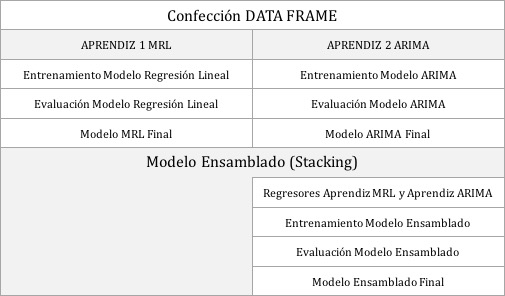
\includegraphics[width=5in]{ArquitecturaModeloEnsamblado}
    \caption{Proceso de Investigación para el Análisis del Modelo Predictivo (Fuente Propia)}
\end{figure}

Cada aprendiz es a su vez un modelo de aprendizaje automatizado con su propia metodología de investigación.

\subsubsection{Aprendiz 1: Modelo de Regresión Lineal}
\begin{itemize}
	\item El aprendiz 1 es un modelo de regresión lineal utilizando como variable dependiente el valor de la TRM para cada día del juego de datos y como regresores un arreglo asociado de cotizaciones del precio promedio mundial de los once productos principales de la canasta de exportación de Colombia entre los años 2010 y 2017.
	\item Para el juego de entrenamiento se selecciona un 70\% de los datos disponibles. Dicha selección se hace con la ayuda de la biblioteca CARET de R para funciones de aprendizaje automatizado.
	\item Para el juego de validación se selecciona un 30\% de los datos disponibles. Dicha selección también se hace con la ayuda de la biblioteca CARET de R para funciones de aprendizaje automatizado.
	\item La variable SEED se prefigura al valor arbitrario \emph{7556014} para propósitos de reproducibilidad de los datos.
	\item El aprendizaje automatizado no asegura que todos los regresores sean útiles o necesarios para una predicción dentro de los valores de confianza esperados. Existe la posibilidad que un número limitado de regresores cumpla con los mismos valores de predicción que la totalidad de los mismos y que el modelo generalice mejor al tener menos regresores (disminuyendo la inflación de la varianza como efecto secundario).
	\item Para determinar el número óptimo de regresores se procedió a armar el modelo de aprendizaje automatizado sumando un regresor a la vez y analizando los valores del coeficiente de determinación y coeficiente de correlación. Los valores finales del error mínimo cuadrático de cada modelo se comparan para determinar la mejor combinación de regresores.
	\item Como segunda validación para la combinación correcta de regresores, se utilizó el análisis \emph{Step\_AIC} (reducción óptima de regresores utilizando análisis combinatorio y el Criterio de Información de Aikake) con la biblioteca \emph{STEP\_AIC} de \emph{R}. El método \emph{STEP\_AIC} es intensivo en recursos de computación y no siempre arroja resultados superiores a los que un investigador pueda armar a mano utilizando técnicas visuales de exploración de datos.
\end{itemize}

\subsubsection{Aprendiz 2: Modelo ARIMA}
\begin{itemize}
	\item El aprendiz 2 es un modelo de pronostico ARIMA utilizando como serie de tiempo el valor de la TRM para cada día del juego de datos entre los años 2010 y 2017.
	\item Para el juego de entrenamiento se selecciona un 70\% de los datos disponibles. Dicha selección se hace con la ayuda de la biblioteca FORECAST de R para funciones de aprendizaje automatizado utilizando series de tiempo \cite{hyndman}.
	\item Para el juego de validación se selecciona un 30\% de los datos disponibles. Dicha selección también se hace con la ayuda de la biblioteca FORECAST de R para funciones de aprendizaje automatizado de series de tiempo.
	\item La variable SEED se prefigura al valor arbitrario \emph{7556014} para propósitos de reproducibilidad de los datos.
\end{itemize}

\subsubsection{Clasificador Ensamblado}
\begin{itemize}
	\item El clasificador ensamblado se toma como un arreglo de una variable dependiente (el valor de la TRM para cada día correspondiente al juego de datos) y dos variables independientes (los resultados de la predicción de los dos aprendices).
	\item Para el juego de entrenamiento se selecciona el 100\% de los datos disponibles. Dicha selección se hace con los resultados de las pruebas de evaluación de los dos aprendices iniciales \cite{popularEnsemble}.
	\item La variable SEED se prefigura al valor arbitrario \emph{7556014} para propósitos de reproducibilidad de los datos.
	\item El modelo se resuelve utilizando la metodología de Stacking como un modelo de regresión lineal \cite{smolyakov}.
\end{itemize}

\subsubsection{Validación del Modelo Ensamblado}
Se espera del modelo final un nivel de desempeño con predicciones dentro de un \(\alpha \leq 0.05\). Para tal fin dentro del diseño de investigación se valida el modelo sometiendo el mismo a un juego aleatorio de 100 datos de muestra que comprende:

\subsubsection{Esquema Visual del Modelo Predictivo}
El siguiente es el esquema visual del modelo predictivo donde se muestra como los resultados de los aprendices del modelo ARIMA y de regresión lineal múltiple se convierten en las entradas del modelo ensamblado.

\begin{figure}[H]
	\centering
	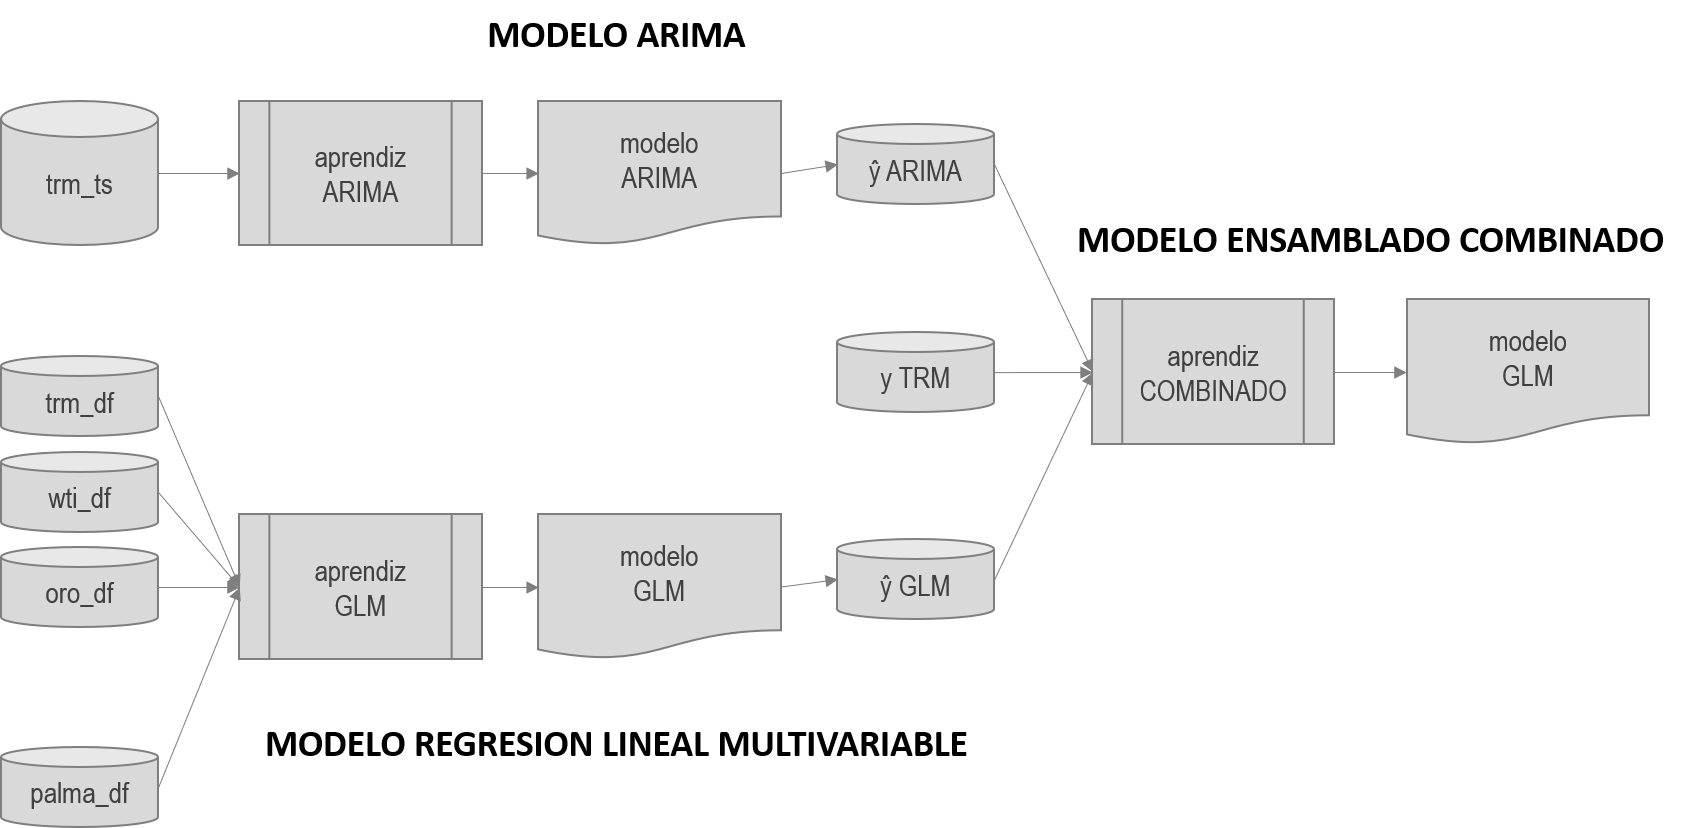
\includegraphics[width=5in]{images/EsquemaModeloPredictivo.png}	\caption{Esquema Modelo Predictivo}
\end{figure}

\begin{itemize}
	\item Resultados de predicción del modelo versus el modelo aprendiz 1 de regresión lineal multivariable.
	\item Resultados de predicción del modelo ensamblado versus el modelo aprendiz 2 ARIMA.
	\item Resultados de predicción del modelo ensamblado versus un intervalo de confianza del 99\%.
\end{itemize}

El modelo se considera óptimo para producción si pasa las tres pruebas de validación.

\section{Diseño de la Instrumentación}
El diseño de la instrumentación para el trabajo de laboratorio incluirá programas de software matemático para:

\begin{itemize}
    \item Recolectar las diferentes series de tiempo que servirán como variables dependientes (valor de la TRM) e independientes (regresores tales como las cotizaciones del barril de petróleo, quintal de café, etc.)
    \item Análisis exploratorio visual para determinar validez de los datos, muestras de autocorrelación y autocorrelación parcial a través de la prueba Dickey-Fueller
    \item Calce de la función de regresión lineal para las variables independientes
    \item Código para el modelo predictivo ensamblado
\end{itemize}

\subsection{Componentes de Investigación Series de Tiempo}
Un componente de aportación es cualquier rubro que se supone se exporta desde Colombia, aporta ingresos en dólares, y por lo tanto ayuda a equilibrar la balanza de pagos y demanda demanda de divisas - y por ende la TRM. Es importante hacer un análisis de cada uno de estos que debe incluir \cite{zumelMount}:

\begin{itemize}
	\item carga inicial como serie de tiempo (time series class)
	\item start(), end()
    \item summary()
    \item plot.ts()
    \item acf()
    \item pacf()
    \item descomponer en stl()
    \item prueba Dickey Fuller adf.test()
\end{itemize}

La carga inicial de datos para cualquier serie de tiempo se hace a través del servicio web de \textit{Quandl} (el siguiente ejemplo ilustrativo utiliza las cotizaciones del quintal de café).

\begin{lstlisting}[language=R]
# Load coffee prices as time series
library(Quandl)
library(tseries)

Quandl.api_key("KzzS8Vfxkw1ZgTWgU4jH")
coffee <- Quandl("ODA/PCOFFOTM_USD", collapse = "monthly", type = "ts")
head(coffee)
class(coffee)
cycle(coffee)
\end{lstlisting}

\subsection{EDA (Explorative Data Analysis)}
La forma más sencilla de ver los efectos del precio del café es revisar la tendencia del precio internacional y si ha habido efectos por temporada o alguna tendencia \cite{daroczi}.

\begin{lstlisting}[language=R]
plot.ts(coffee)
abline(reg = lm(coffee ~ time(coffee)))
\end{lstlisting}

\begin{figure}[H]
	\centering
	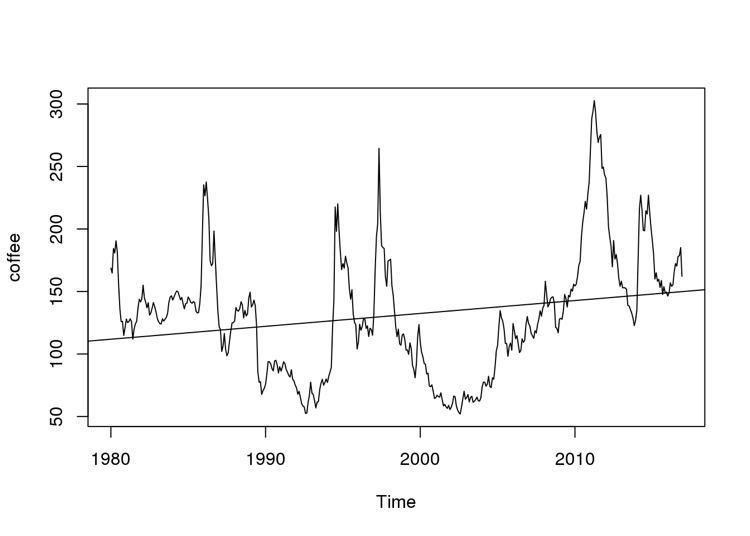
\includegraphics[width=5in]{correlacionTiempoCafe}
	\caption{Análisis EDA Cotización Internacional Café por quintal  (Fuente Propia)}
\end{figure}

Otro examen necesario es el de autocorrelación y autocorrelación parcial. Ambos análisis nos permiten ver si la serie es del tipo auto-regresiva o de promedios móviles \cite{hyndman}.

\begin{lstlisting}[language=R]
par(mfrow=c(1,2))
acf(coffee)
pacf(coffee)
\end{lstlisting}

\begin{figure}[H]
	\centering
	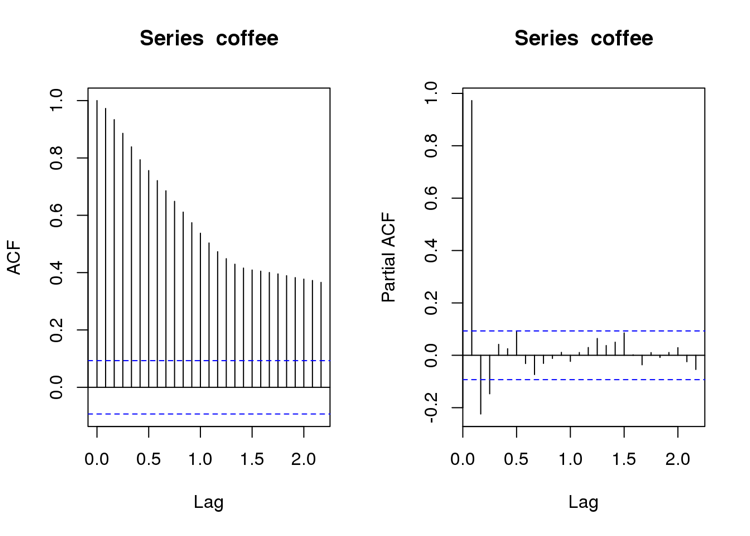
\includegraphics[width=5in]{autocorrelacion}\\
	\caption{Correlograma Precio Internacional del Café (Fuente Propia)}
\end{figure}

El último examen es la descomposición de la serie en datos, temporalidad y tendencia, para ver si alguno de estos elementos está presente.

\begin{lstlisting}[language=R]
decomp <- stl(coffee, s.window = 11)
plot(decomp)
\end{lstlisting}

\begin{figure}[H]
	\centering
	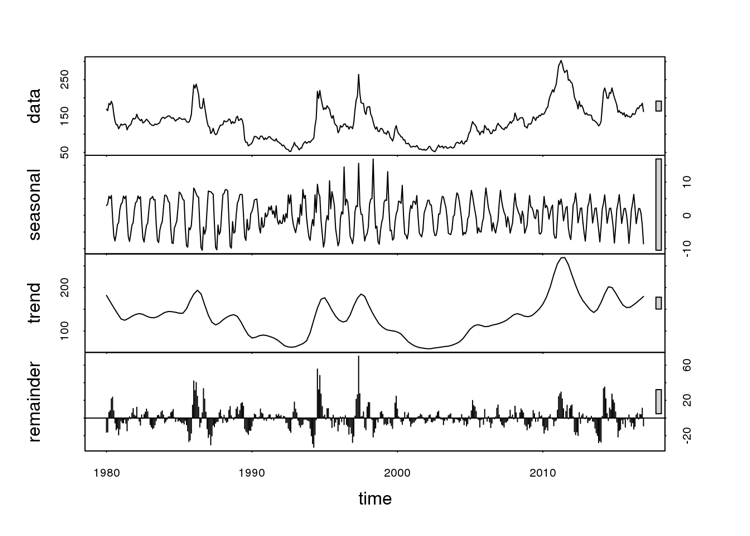
\includegraphics[width=5in]{decopSTLCafe}\\
	\caption{Descomposición STL Precio Internacional del Café (Fuente Propia)}
\end{figure}

El test \emph{Dickey Fuller} \cite{dickeyfuller} es la prueba mas importante para la verificación de la estacionalidad de una serie de tiempos. La literatura recomienda altamente someter todas las pruebas de series al test \emph{Dickey Fuller} antes de proceder con otros análisis \cite{hyndman}.

\begin{lstlisting}[language=R]
# Dickey Fuller Test for stationary time series
df <- adf.test(coffee, k = 12)
df$statistic
df$p.value
\end{lstlisting}

\subsection{Regresión Lineal con Calce de la Función de Predicción}
Los modelos de regresión lineal utilizan la biblioteca \emph{Quandl} para la extracción de datos y deben hacer la transformación del arreglo de datos a una serie de tiempos. Los datos serán colapsados de forma mensual y se revisará la fórmula de la función de calce para el coeficiente de correlación y determinación \cite{narayanachar}.

\begin{lstlisting}[language=R]
# Load oil prices as time series
library(Quandl)
library(tseries)

Quandl.api_key("KzzS8Vfxkw1ZgTWgU4jH")
wti <- Quandl("EIA/PET_RWTC_D", collapse = "monthly", type = "ts")
head(wti)
class(wti)
cycle(wti)

plot.ts(wti)
abline(reg = lm(wti ~ time(wti)), col="red")
fit = lm(wti ~ time(wti))
summary(fit)


Call:
lm(formula = wti ~ time(wti))

Residuals:
    Min      1Q  Median      3Q     Max
-45.031 -13.929  -0.368  11.399  80.925

Coefficients:
              Estimate Std. Error t value Pr(>|t|)
(Intercept) -4849.3862   213.2634  -22.74   <2e-16 ***
time(wti)       2.4439     0.1065   22.94   <2e-16 ***
---
Signif. codes:  0 '***' 0.001 '**' 0.01 '*' 0.05 '.' 0.1 ' ' 1

Residual standard error: 19.43 on 384 degrees of freedom
Multiple R-squared:  0.5782,	Adjusted R-squared:  0.5771
F-statistic: 526.4 on 1 and 384 DF,  p-value: < 2.2e-16
\end{lstlisting}

\begin{figure}[H]
	\centering
	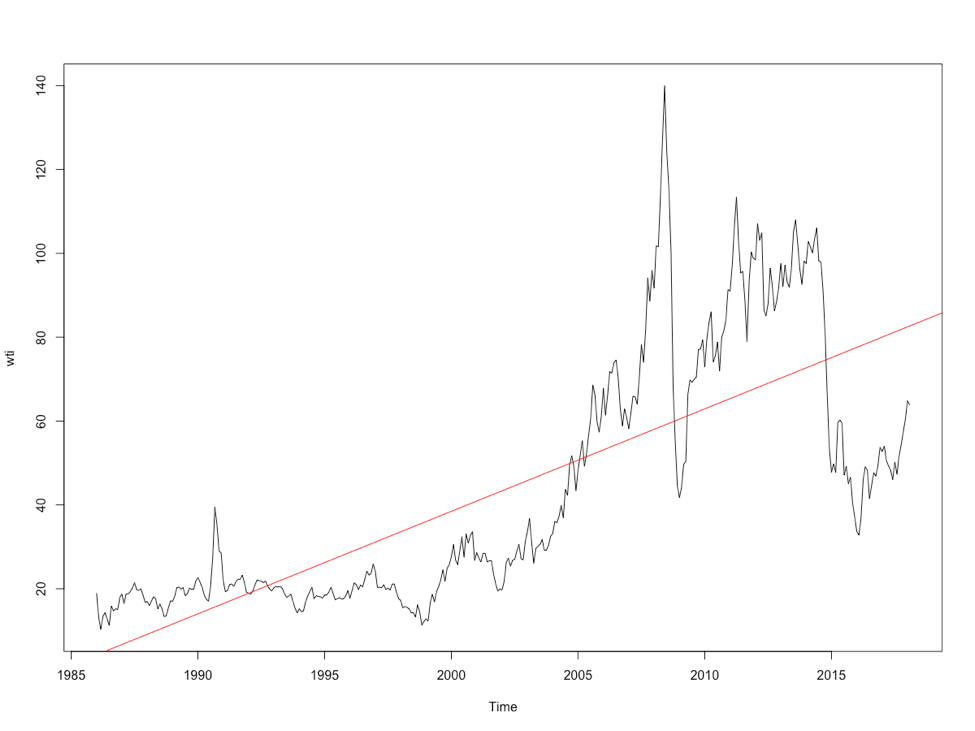
\includegraphics[width=5in]{regresionTiempoWTI}\\
	\caption{Descomposición STL Precio Internacional del Café (Fuente Propia)}
\end{figure}

\subsection{Modelo Predictivo Ensamblado}
El modelo predictivo ensamblado es el resultado del entrenamiento de un modelo predictivo de regresión lineal y un modelo ARIMA. Ambos modelos se combinan y se entrenan con la variable de valor real en común para ambos \cite{viswanathan}.

\begin{lstlisting}[language=R]
# Pseudo-codigo R simplificado
# Funcion de modelo ensamblado

# Cargar Data Frame con informacion de series de tiempo
library(caret)
set.seed(7556014)
data(featuresTRM)
data(TRM)
adData = data.frame(TRM, featuresTRM)
inTrain = createDataPartition(adData$TRM, p = 3/4)[[1]]
training = adData[ inTrain,]
testing = adData[-inTrain,]

set.seed(7556014)

modelo1 <- train(TRM ~ ., method = "glm", data = training)
modelo2 <- train(TRM ~ ., method = "ARIMA", data = training)

# Vectores de valores de prediccion de cada modelo
predVec1 <- predict(modelo1, testing)
predVec2 <- predict(modelo2, testing)

# Construccion de matriz de datos ensamblados (variable dependiente y predictor)
predDF <- data.frame(TRM = testing$TRM, predVec1, predVec2)

# Modelo combinado (fit)
combModelFit <- train(TRM ~ ., method = "glm", data = predDF)
finalPred <- predict(combModelFit, predDF)
\end{lstlisting}

\section{Diseño de muestreo}

Inicialmente, podemos calcular el tamaño de la muestra necesaria para nuestro estudio con la fórmula \cite{mendehall}:

\begin{equation}
   n =  (N* z^2*p*q)/(E^2*(N-1)+ z^2*p*q)
\end{equation}

El tamaño total de todas las cotizaciones de la TRM o del precio internacional del petróleo WTI es un número finito. Los mercados funcionan de lunes a viernes, por lo general las cincuenta y dos semanas del año. Para el uso común de la tasa de cambio, esta cifra se usa todos los días, por ejemplo cuando un consumidor usa una tarjeta de crédito y el banco debe referir al valor de la TRM aunque no sea día de operaciones bursátiles. Por lo que el número total de posibles cotizaciones oficiales en un año dado cualesquiera se determinan como:

\begin{equation}
    N_{regresor} = 365
\end{equation}

La fórmula es muy simple y equivale a sustituir cualquier variable regresor (por ejemplo, el valor del petróleo WTI) por los números reales de días del año.

\begin{equation}
    N_{wti} = 365
\end{equation}

Ende, existen 365 posibles valores de la cotización del petróleo WTI en un año cualesquiera. Dado que el modelo de predicción de aprendizaje automatizado utiliza datos del año 2010 al 2017 inclusive, podemos ampliar el universo dentro del período de estudio con la siguiente formula:
\begin{equation}
    n_{regresor} = 365 * 8 = 2920
\end{equation}

Nuestro universo por regresor equivale a dos mil novecientos veinte puntos de datos. Para un estudio con un nivel de confianza del 99\% y un error de estimación del 5\% calculamos el número de la muestra como una proporción, donde:

\begin{eqnarray*}
  N &=& 2,080 \text{ puntos de datos} \\
  p &=& 0.5 \\
  q &=& 0.5 \text{ o (1 – p)} \\
  z &=& 99\% \text{ o 2.575} \\
  e &=& 5\% \text{ o 0.05} \\
\end{eqnarray*}

Utilizamos el lenguaje R para resolver el cálculo:

\begin{lstlisting}[language=R]
N <- 2080
p <- 0.5
q <- 1 - p
z <- 2.575
E <- 0.05

muestra <- (N * z^2 * p * q) / ((N - 1) * E^2 + z^2 * p * q)
muestra
[1] 502.9681
\end{lstlisting}

El tamaño de la muestra es 503 puntos de datos por regresor a utilizar. Sin embargo, dado que los usos de técnicas de Ciencia de Datos nos permiten acceder a la biblioteca Quandl de forma de recolectar el universo entero de datos, utilizaremos los 2,920 puntos de datos para cada regresor, trabajando de esta forma con el universo entero y no la muestra. Este es un buen ejemplo del uso de Big Data \cite{pengMatsui} que no solo aplica a muestras grandes de universos extensos, sino al total de la data de un universo pequeño.

\subsubsection{Reglas de Imputación de Datos}
Es común que las bases de datos retornen series de datos incompletas para los días feriados o días sin cambio en la cotización del bien. Para determinar el valor de cualquier día incompleto, la investigación resolvió el método de imputación como la última cotización válida para el regresor.

\subsection{Observaciones Adicionales Sobre el Uso de Muestras dentro de Diseños de Investigación con Regresión Lineal}
No todos los autores están de acuerdo con el uso de la fórmula tradicional para el cálculo del número de muestras en un estudio de regresión lineal. William Dupont y Walton Plummer han discutido el uso de técnicas alternativas cuando los estudios (sobre todo los estudios clínicos) utilizan regresiones lineales multivariable \cite{dupontPlummer}. Dichas técnicas se apoyan en la identificación de diferentes pendientes en los análisis de regresión versus el uso de coeficientes (argumentando que es más fácil comparar visualmente pendientes versus coeficientes) y el manejo del poder estadístico $1 – \beta$. Sobre este último los autores manifiestan ajustar los niveles de poder para verificar en que momento del cambio se detecta diferencias de la pendiente de una hipótesis contra su hipótesis alternativa dentro de una muestra de n pacientes.

Al momento de preparar el diseño del estudio, las herramientas de medición y la muestra, el doctorando ha decidido no profundizar más en métodos menos tradicionales de cálculo de muestras en estudios de regresión lineal, dado que en el caso específico se utilizará la totalidad del universo, haciendo el cálculo de muestra innecesario.

\setcounter{chapter}{3}
\chapter{Resultados}
Contenidos por definir.

\chapter{Conclusiones y Recomendaciones}
La conclusión principal de la investigación doctoral es que los rubros de exportación de la economía Colombiana pueden ser utilizado como regresores de un modelo predictivo de la tasa de referencia del mercado. Cuando estos regresores se combinan con la serie de tiempo de la TRM misma a través del uso del aprendizaje automatizado, el resultado es un modelo ensamblado combinado parsimonioso y altamente preciso.

Cuando elevamos el nivel de análisis alrededor de los resultados del trabajo de laboratorio podemos ver conclusiones enfocadas en tres rubros:

\begin{enumerate}
  \item conclusiones específicas sobre el uso y validez de cada método de predicción utilizado en el aprendizaje automatizado como aprendiz
  \item conclusiones específicas sobre las ventajas de la metodología de métodos ensamblados
  \item conclusiones del uso de aprendizaje automatizado en la contabilidad de costos
\end{enumerate}

La Ciencia de Datos y el Aprendizaje Automatizado como disciplinas son áreas de la academia relativamente nuevas y con menor exposición en las universidades Latinoamericanas. El trabajo de investigación doctoral nos permite aportar recomendaciones al respecto de los siguientes temas:

\begin{itemize}
  \item recomendaciones sobre la implementación de una investigación de Ciencia de Datos utilizando Aprendizaje Automatizado
  \item recomendaciones sobre futuros trabajos de investigación resultantes de inquietudes que surgieron a lo largo del trabajo de laboratorio y a las cuales no se les pudo dar respuestas que satisfagan la curiosidad científica
\end{itemize}

\section{Conclusiones}
Cada método de aprendizaje automatizado utilizado en el siguiente trabajo de investigación tiene sus bondades. Para discutir cada uno con total objetividad, haremos referencia a una sola tabla comparativa de valores de desempeño y precisión.

\begin{table}[h!]
  \begin{center}
    \caption{Desempeño Comparativo de Métodos Machine Learning}
    \label{tab:table1}
    \begin{tabular}{c|c|c|c}
      \textbf{Indicador} & \textbf{ARIMA} & \textbf{Regresión Lineal} & \textbf{Modelo Ensamblado}\\
      \hline
      RMSE & 25.5473 &89.0524 & 24.8040 \\
      R2 & 0.9976 & 0.9714 & 0.9978 \\
    \end{tabular}
  \end{center}
\end{table}

\subsection{Modelo ARIMA}
El modelo ARIMA tuvo resultados por encima de las expectativas del investigador, con un valor de error cuadrático bajo y un valor de coeficiente de determinación alto, ciertamente superior al método de regresión lineal multivariable. La fortaleza del pronóstico ARIMA se fundamente en lo completo y robusto del juego de datos utilizado. La serie de tiempo de la TRM es estudiada por todo el sector contable, económico y financiero de Colombia, por lo que no fue sorpresa que de todas las series de datos está fuera la más accesible de estudio. El comportamiento de la serie de datos TRM también tienen una tendencia secular y de estacionalidad muy marcadas que se ajusta al uso de metodologías como ARIMA.

Dado el caso de no contar con otras metodologías o acceso a base de datos mayores para ampliar el rango de métodos potables, el uso de un aprendiz ARIMA puede solucionar el problema de pronosticar el valor futuro de la TRM sin necesidad de mayor complicación.

\subsection{Modelo de Regresión Lineal Multivariable}
El modelo de regresión lineal multivariable tuvo el desempeño menos preciso de los tres métodos estudiados. El valor del error cuadrático fue el mayor de los tres (aunque no necesariamente se puede decir que fue alto) y el coeficiente de determinación fue el menor de los tres (aunque fue alto estadísticamente hablando). El uso de los rubros de exportación como regresores se justifica con el calce ajustado del modelo, por lo que se considera un modelo robusto y parsimonioso. Sin embargo es un modelo más difícil de aplicar sin conocimientos de programación de métodos de aprendizaje automatizado y no rindió mejores pronósticos que el uso más sencillo de ARIMA.

\subsection{Modelo Ensamblado Stacking}
Correspondiendo con la literatura y los trabajos de autores como Daroczi, Leek, Peng y Tattar, el modelo ensamblado tuvo los mejores niveles de desempeño y precisión con el error cuadrático más bajo y el coeficiente de determinación más alto. La utilización de los dos métodos iniciales como entradas para un aprendiz ensamblado genera un método más robusto que se nutre de entradas pre-procesadas por los aprendices que las componen. Habiendo dicho esto, el desempeño obtenido por el método ensamblado no se puede considerar sino marginal en comparación con los aprendices que lo alimentan. La diferencia del error cuadrático es considerable si se mide contra el aprendiz de regresión lineal multivariable, pero poco notable contra el aprendiz ARIMA. De la misma forma, el valor del coeficiente de determinación su superior por menos de 0.026 contra el aprendiz de regresión lineal multivariable, pero nuevamente imperceptible versus el aprendiz ARIMA.

\subsection{Modelos de Aprendizaje Automatizado versus Modelos Ensamblados}
La utilización de la TRM en contratos de futuros o \emph{forwards} puede justificar la complejidad adicional de implementar un algoritmo compuesto. Para funciones de análisis de costos el overhead adicional de lidiar con un modelo ensamblado puede no hacer diferencias en el costeo final, sobre todo en cifras con redondeos a 2 decimales.

Para la organización moderna y de amplio alcance la complejidad adicional de la utilización de modelos ensamblados puede verse recompensada con el tiempo. El mayor nivel de precisión siempre redundará en mejores márgenes de utilidad y ganancias de productividad. En un ambiente dinámico y de bajo margen de utilidad como lo es el negocio de corretaje bursátil dicha precisión puede ser la diferencia entre la viabilidad de operación o no.

Para reportes ad-hoc, análisis de factibilidad, o toma rápida de decisiones, el uso de modelos ensamblados puede no ser la mejor respuesta. El trabajo de investigación doctoral llegó a un modelo parsimonioso y preciso con el uso del modelo ARIMA, el más sencillo de los tres de aplicar y entender. En el caso de tener que afrontar pronósticos de mediana exactitud, un modelo simple y rápido de aplicar puede satisfacer a la organización mejor que uno de mayor precisión pero intensivo en el uso de recursos y bases de datos extensas y validadas.

\section{Recomendaciones}
El trabajo de investigación arroja recomendaciones sobre la implementación de una investigación de Ciencia de Datos utilizando Aprendizaje Automatizado, y recomendaciones sobre futuros trabajos de investigación resultantes de inquietudes que surgieron a lo largo del trabajo de laboratorio.

\subsection{Implementación de Investigación de un Modelo Predictivo de Aprendizaje Automatizado}
Todas las fuentes de datos y todo el código fuente utilizado en el trabajo doctoral puede ubicarse en el sitio \emph{Github} del investigador. Ambos pueden ser utilizados bajo licencia MIT Open Source por cualquier estudiante, ejecutivo o persona que quiere conocer, ampliar, replicar, corroborar, mejorar y/o ampliar el conocimiento sobre la Ciencia de Datos y el Aprendizaje Automatizado.

Empero, utilizar el código provisto desde un computador personal es muy diferente a desplegar una investigación de Ciencia de Datos. Si para otros investigadores la recopilación de la información puede ser un problema crítico y el diseño de la instrumentación una decisión difícil para asegurar un análisis exitoso, el científico de datos se encuentra con problemas diferentes y típicos de su rama. La cantidad de datos disponible para cada investigación por lo general es exagerada y disponible con facilidad (razón por la cual se acuña el término BIG DATA). El problema pasa de la recolección al procesamiento de los datos. De igual manera el diseño de la instrumentación fue facilitado por la existencia de cientos de librerías disponibles en el lenguaje R. El investigador de datos pasa más tiempo decidiendo que juegos de datos son aplicables al


%% BIBLIOGRAPHY
\bibliographystyle{apalike}
\pagebreak
\bibliography{thesis.bib}

\setcounter{chapter}{6}
\chapter{Otras Fuentes}
Contenidos por definir.

\setcounter{chapter}{7}
\chapter{Anexos}


\section{Bibliotecas de Programas}
La siguiente sección recopila los programas utilizados para el trabajo de investigación doctoral.

\subsection{Programa buildTRM.R}
El siguiente listado de secuencia de comandos R construye la serie de tiempos TRM para la tasa representativa del mercado.

\begin{lstlisting}[language=R]
# UBJ Doctorado en Administracion Gerencial
# Modelo Predictivo de la TRM Utilizando Machine Learning
# LIB ubj/code/buildTRM.R 
# FECHA 19/08/2018
# Ariel E. Meilij
#
# BRIEF Construye serie de datos TRM

library(Quandl)
library(tseries)
library(ggplot2)
library(ggfortify)
library(Hmisc)
library(corrplot)
library(PerformanceAnalytics)
library(reshape2)
library(ggpubr)

Quandl.api_key("KzzS8Vfxkw1ZgTWgU4jH")
trm_data <- Quandl("CURRFX/USDCOP")

# Limpiar serie de tiempo TRM en su data.frame
trm <- trm_data[, 1:2]
trm <- subset(trm, trm$Date > "2009-12-31")
trm <- subset(trm, trm$Rate > 1500)
colnames(trm) <- c("Date", "trm")

fechas <- seq(as.Date("2010-01-01"), as.Date("2017-12-31"), "days")
quote <- c(1:2922)
# Cargar como valor inicial valor mas antiguo de la serie de tiempo
last_quote <- trm[dim(trm)[1],2]

for(i in 1:2922)
{if(length(trm[which(trm$Date == fechas[i]), ]$trm))
{quote[i] <- trm[which(trm$Date == fechas[i]), ]$trm
last_quote <- trm[which(trm$Date == fechas[i]), ]$trm}
  else
  {quote[i] <- last_quote}
}

# Build into a time series
trm_ts <- ts(quote, start=c(2010,1,1), frequency=365)
plot(decompose(trm_ts))
save(trm_ts, file = "data/trm_ts")

# Build into data frame
trm_df <- data.frame(fechas, quote)
colnames(trm_df) = c("Date", "trm")
save(trm_df, file = "data/trm_df")
# EOC
\end{lstlisting}

\subsection{Programa buildBanana.R}
El siguiente listado de secuencia de comandos R construye la serie de tiempos banana con los valores de las cotizaciones mundiales de la tonelada de guineo.

\begin{lstlisting}[language=R]
# UBJ Doctorado en Administracion Gerencial
# Modelo Predictivo de la TRM Utilizando Machine Learning
# LIB ubj/code/buildBanana.R 
# FECHA 19/08/2018
# Ariel E. Meilij
#
# BRIEF Construye serie de datos del banano

library(Quandl)
library(tseries)
library(ggplot2)
library(ggfortify)
library(Hmisc)
library(corrplot)
library(PerformanceAnalytics)
library(reshape2)
library(ggpubr)

Quandl.api_key("KzzS8Vfxkw1ZgTWgU4jH")
banana_data <- Quandl("ODA/PBANSOP_USD")

# Limpiar serie de tiempo banana en su data.frame
banana <- subset(banana_data, banana_data$Date > "2009-12-31")
colnames(banana) <- c("Date", "banana")

fechas <- seq(as.Date("2010-01-01"), as.Date("2017-12-31"), "days")
quote <- c(1:2922)
# Cargar como valor inicial valor mas antiguo de la serie de tiempo
last_quote <- banana[dim(banana)[1],2]

for(i in 1:2922)
{if(length(banana[which(banana$Date == fechas[i]), ]$banana))
{quote[i] <- banana[which(banana$Date == fechas[i]), ]$banana
last_quote <- banana[which(banana$Date == fechas[i]), ]$banana}
  else
  {quote[i] <- last_quote}
}

# Build into a time series
banana_ts <- ts(quote, start=c(2010,1,1), end=c(2017,12,31), frequency=365)
plot(decompose(banana_ts))
save(banana_ts, file = "data/banana_ts")

# Build into data frame
banana_df <- data.frame(fechas, quote)
colnames(banana_df) = c("Date", "banana")
save(banana_df, file = "data/banana_df")
# EOC
\end{lstlisting}

\subsection{Programa buildCafe.R}
El siguiente listado de secuencia de comandos R construye la serie de tiempos café con los valores de las cotizaciones mundiales de la tonelada de café Arabiga.

\begin{lstlisting}[language=R]
# UBJ Doctorado en Administracion Gerencial
# Modelo Predictivo de la TRM Utilizando Machine Learning
# LIB ubj/code/buildCafe.R 
# FECHA 19/08/2018
# Ariel E. Meilij
#
# BRIEF Construye serie de datos cafe

library(Quandl)
library(tseries)
library(ggplot2)
library(ggfortify)
library(Hmisc)
library(corrplot)
library(PerformanceAnalytics)
library(reshape2)
library(ggpubr)

Quandl.api_key("KzzS8Vfxkw1ZgTWgU4jH")
cafe_data <- Quandl("CHRIS/ICE_KC1")

# Limpiar serie de tiempo cafe en su data.frame
cafe <- cafe_data[,c(1,5)]
cafe <- subset(cafe, cafe$Date > "2009-12-31")
cafe <- na.omit(cafe)
colnames(cafe) <- c("Date", "cafe")

fechas <- seq(as.Date("2010-01-01"), as.Date("2017-12-31"), "days")
quote <- c(1:2922)
# Cargar como valor inicial valor mas antiguo de la serie de tiempo
last_quote <- cafe[dim(cafe)[1],2]

for(i in 1:2922)
{if(length(cafe[which(cafe$Date == fechas[i]), ]$cafe))
{quote[i] <- cafe[which(cafe$Date == fechas[i]), ]$cafe
last_quote <- cafe[which(cafe$Date == fechas[i]), ]$cafe}
  else
  {quote[i] <- last_quote}
}

# Build into a time series
cafe_ts <- ts(quote, start=c(2010,1,1), end=c(2017,12,31), frequency=365)
plot(decompose(cafe_ts))
save(cafe_ts, file = "data/cafe_ts")

# Build into data frame
cafe_df <- data.frame(fechas, quote)
colnames(cafe_df) = c("Date", "cafe")
save(cafe_df, file = "data/cafe_df")
# EOC
\end{lstlisting}

\subsection{Programa buildCarbon.R}
El siguiente listado construye la serie de tiempos carbón con los precios de las cotizaciones mundiales de la tonelada de carbón.

\begin{lstlisting}[language=R]
# UBJ Doctorado en Administracion Gerencial
# Modelo Predictivo de la TRM Utilizando Machine Learning
# LIB ubj/code/buildCarbon.R 
# FECHA 19/08/2018
# Ariel E. Meilij
#
# BRIEF Construye serie de datos carbon

library(Quandl)
library(tseries)
library(ggplot2)
library(ggfortify)
library(Hmisc)
library(corrplot)
library(PerformanceAnalytics)
library(reshape2)
library(ggpubr)

Quandl.api_key("KzzS8Vfxkw1ZgTWgU4jH")
carbon_data <- Quandl("EIA/COAL")

# Limpiar serie de tiempo CARBON en su data.frame
carbon <- carbon_data[, 1:2]
carbon <- subset(carbon, carbon$`Week Ended` > "2009-12-31")
colnames(carbon) <- c("Date", "carbon")

fechas <- seq(as.Date("2010-01-01"), as.Date("2017-12-31"), "days")
quote <- c(1:2922)
# Cargar como valor inicial valor mas antiguo de la serie de tiempo
last_quote <- carbon[dim(carbon)[1],2]

for(i in 1:2922)
{if(length(carbon[which(carbon$Date == fechas[i]), ]$carbon))
{quote[i] <- carbon[which(carbon$Date == fechas[i]), ]$carbon
last_quote <- carbon[which(carbon$Date == fechas[i]), ]$carbon}
  else
  {quote[i] <- last_quote}
}

# Build into a time series
carbon_ts <- ts(quote, start=c(2010,1,1), end=c(2017,12,31), frequency=365)
plot(decompose(carbon_ts))
save(carbon_ts, file = "data/carbon_ts")

# Build into data frame
carbon_df <- data.frame(fechas, quote)
colnames(carbon_df) = c("Date", "carbon")
save(carbon_df, file = "data/carbon_df")
# EOC
\end{lstlisting}

\subsection{Programa buildGasoil.R}
El siguiente programa construye la serie de tiempo gasoil con los precios internacionales del gasoil en galones.

\begin{lstlisting}[language=R]
# UBJ Doctorado en Administracion Gerencial
# Modelo Predictivo de la TRM Utilizando Machine Learning
# LIB ubj/code/buildgasoil.R 
# FECHA 19/08/2018
# Ariel E. Meilij
#
# BRIEF Construye serie de datos del banano

library(Quandl)
library(tseries)
library(ggplot2)
library(ggfortify)
library(Hmisc)
library(corrplot)
library(PerformanceAnalytics)
library(reshape2)
library(ggpubr)

Quandl.api_key("KzzS8Vfxkw1ZgTWgU4jH")
gasoil_data <- Quandl("NASDAQOMX/NQCIGOER")

# Limpiar serie de tiempo gasoil en su data.frame
gasoil <- gasoil_data[, c(1:2)]
gasoil <- subset(gasoil, gasoil$`Trade Date` > "2009-12-31")
gasoil <- subset(gasoil, gasoil$`Index Value` > 0)
colnames(gasoil) <- c("Date", "gasoil")

fechas <- seq(as.Date("2010-01-01"), as.Date("2017-12-31"), "days")
quote <- c(1:2922)
# Cargar como valor inicial valor mas antiguo de la serie de tiempo
last_quote <- gasoil[dim(gasoil)[1],2]

for(i in 1:2922)
{if(length(gasoil[which(gasoil$Date == fechas[i]), ]$gasoil))
{quote[i] <- gasoil[which(gasoil$Date == fechas[i]), ]$gasoil
last_quote <- gasoil[which(gasoil$Date == fechas[i]), ]$gasoil}
  else
  {quote[i] <- last_quote}
}

# Build into a time series
gasoil_ts <- ts(quote, start=c(2010,1,1), end=c(2017,12,31), frequency=365)
plot(decompose(gasoil_ts))
save(gasoil_ts, file = "data/gasoil_ts")

# Build into data frame
gasoil_df <- data.frame(fechas, quote)
colnames(gasoil_df) = c("Date", "gasoil")
save(gasoil_df, file = "data/gasoil_df")
# EOC
\end{lstlisting}

\subsection{Programa buildHulla.R}
El siguiente programa construye la serie de tiempo hulla con las cotizaciones mundiales de la tonelada métrica de hulla térmica. 

\begin{lstlisting}[language=R]
# UBJ Doctorado en Administracion Gerencial
# Modelo Predictivo de la TRM Utilizando Machine Learning
# LIB ubj/code/buildHulla.R 
# FECHA 19/08/2018
# Ariel E. Meilij
#
# BRIEF Construye serie de datos hulla termica

library(Quandl)
library(tseries)
library(ggplot2)
library(ggfortify)
library(Hmisc)
library(corrplot)
library(PerformanceAnalytics)
library(reshape2)
library(ggpubr)

Quandl.api_key("KzzS8Vfxkw1ZgTWgU4jH")
hulla_data <- Quandl("CHRIS/SGX_CFF3")

# Limpiar serie de tiempo HULLA en su data.frame
hulla <- hulla_data[, c(1,6)]
hulla <- subset(hulla, hulla$Date > "2009-12-31")
colnames(hulla) <- c("Date", "hulla")

fechas <- seq(as.Date("2010-01-01"), as.Date("2017-12-31"), "days")
quote <- c(1:2922)
# Cargar como valor inicial valor mas antiguo de la serie de tiempo
last_quote <- hulla[dim(hulla)[1],2]

for(i in 1:2922)
{if(length(hulla[which(hulla$Date == fechas[i]), ]$hulla))
{quote[i] <- hulla[which(hulla$Date == fechas[i]), ]$hulla
last_quote <- hulla[which(hulla$Date == fechas[i]), ]$hulla}
  else
  {quote[i] <- last_quote}
}

# Build into a time series
hulla_ts <- ts(quote, start=c(2010,1,1), end=c(2017,12,31), frequency=365)
plot(decompose(hulla_ts))
save(hulla_ts, file = "data/hulla_ts")

# Build into data frame
hulla_df <- data.frame(fechas, quote)
colnames(hulla_df) = c("Date", "hulla")
save(hulla_df, file = "data/hulla_df")
# EOC
\end{lstlisting}

\subsection{Programa buildNiquel.R}
El siguiente programa construye la serie de tiempo níquel con las cotizaciones mundiales de la tonelada métrica de ferroníquel.

\begin{lstlisting}[language=R]
# UBJ Doctorado en Administracion Gerencial
# Modelo Predictivo de la TRM Utilizando Machine Learning
# LIB ubj/code/buildNiquel.R 
# FECHA 19/08/2018
# Ariel E. Meilij
#
# BRIEF Construye serie de datos del niquel

library(Quandl)
library(tseries)
library(ggplot2)
library(ggfortify)
library(Hmisc)
library(corrplot)
library(PerformanceAnalytics)
library(reshape2)
library(ggpubr)

Quandl.api_key("KzzS8Vfxkw1ZgTWgU4jH")
niquel_data <- Quandl("ODA/PNICK_USD")
# niquel_data <- Quandl("LME/PR_NI") FUENTE ALTERNA PERO INCOMPLETA

# Limpiar serie de tiempo niquel en su data.frame
# niquel_data <- niquel_data[, c(1,2)]
niquel <- subset(niquel_data, niquel_data$Date > "2009-12-31")
#niquel <- na.omit(niquel)
colnames(niquel) <- c("Date", "niquel")

fechas <- seq(as.Date("2010-01-01"), as.Date("2017-12-31"), "days")
quote <- c(1:2922)
# Cargar como valor inicial valor mas antiguo de la serie de tiempo
last_quote <- niquel[dim(niquel)[1],2]

for(i in 1:2922)
{if(length(niquel[which(niquel$Date == fechas[i]), ]$niquel))
{quote[i] <- niquel[which(niquel$Date == fechas[i]), ]$niquel
last_quote <- niquel[which(niquel$Date == fechas[i]), ]$niquel}
  else
  {quote[i] <- last_quote}
}

# Build into a time series
niquel_ts <- ts(quote, start=c(2010,1,1), end=c(2017,12,31), frequency=365)
plot(decompose(niquel_ts))
save(niquel_ts, file = "data/niquel_ts")

# Build into data frame
niquel_df <- data.frame(fechas, quote)
colnames(niquel_df) = c("Date", "niquel")
save(niquel_df, file = "data/niquel_df")
# EOC
\end{lstlisting}

\subsection{Programa buildOro.R}
El siguiente programa construye la serie de tiempo oro con los precios de cotización de la onza de oro Troy.

\begin{lstlisting}[language=R]
# UBJ Doctorado en Administracion Gerencial
# Modelo Predictivo de la TRM Utilizando Machine Learning
# LIB ubj/code/buildOro.R 
# FECHA 19/08/2018
# Ariel E. Meilij
#
# BRIEF Construye serie de datos oro

library(Quandl)
library(tseries)
library(ggplot2)
library(ggfortify)
library(Hmisc)
library(corrplot)
library(PerformanceAnalytics)
library(reshape2)
library(ggpubr)

Quandl.api_key("KzzS8Vfxkw1ZgTWgU4jH")
gold_data <- Quandl("WGC/GOLD_DAILY_USD")

# Limpiar serie de tiempo GOLD en su data.frame
oro <- subset(gold_data, gold_data$Date > "2009-12-31")
colnames(oro) <- c("Date", "oro")

fechas <- seq(as.Date("2010-01-01"), as.Date("2017-12-31"), "days")
quote <- c(1:2922)
# Cargar como valor inicial valor mas antiguo de la serie de tiempo
last_quote <- oro[dim(oro)[1],2]

for(i in 1:2922)
{if(length(oro[which(oro$Date == fechas[i]), ]$oro))
{quote[i] <- oro[which(oro$Date == fechas[i]), ]$oro
last_quote <- oro[which(oro$Date == fechas[i]), ]$oro}
  else
  {quote[i] <- last_quote}
}

# Build into a time series
oro_ts <- ts(quote, start=c(2010,1,1), end=c(2017,12,31), frequency=365)
plot(decompose(oro_ts))
save(oro_ts, file = "data/oro_ts")

# Build into data frame
oro_df <- data.frame(fechas, quote)
colnames(oro_df) = c("Date", "oro")
save(oro_df, file = "data/oro_df")
# EOC
\end{lstlisting}

\subsection{Programa buildPalma.R}
El siguiente programa construye la serie de tiempo palma, con las cotizaciones mundiales del galón de aceite de palma.

\begin{lstlisting}[language=R]
# buildPalma.R
# 2018-08-15
# Ariel E. Meilij
# UBJ - DBA

# Build palm oil time series and expand
# 2010-01-01 thru 2017-12-31
# Fill-in NA's or 0 values
# Last known quote takes precedence

library(Quandl)
library(tseries)
library(ggplot2)
library(ggfortify)
library(Hmisc)
library(corrplot)
library(PerformanceAnalytics)
library(reshape2)
library(ggpubr)

Quandl.api_key("KzzS8Vfxkw1ZgTWgU4jH")
palma_data <- Quandl("ODA/PPOIL_USD")

palma <- subset(palma_data, palma_data$Date > "2009-12-01")
colnames(palma) <- c("Date", "palma")

fechas <- seq(as.Date("2010-01-01"), as.Date("2017-12-31"), "days")
quote <- c(1:2922)
last_quote <- palma[dim(palma)[1],2]

for(i in 1:2922)
{if(length(palma[which(palma$Date == fechas[i]), ]$palma))
  {quote[i] <- palma[which(palma$Date == fechas[i]), ]$palma
  last_quote <- palma[which(palma$Date == fechas[i]), ]$palma}
      else
  {quote[i] <- last_quote}
}

qplot(x = fechas, y = quote, geom = "line", main = "Cotizacion Aceite de Palma (2010-2017)")

# Build into a time series
palma_ts <- ts(quote, start=c(2010,1,1), end=c(2017,12,31), frequency=365)
plot(decompose(palma_ts))
save(palma_ts, file = "data/palma_ts")

# Build into data frame
palma_df <- data.frame(fechas, quote)
colnames(palma_df) = c("Date", "palma")
save(palma_df, file = "data/palma_df")

# EOC
\end{lstlisting}

\subsection{Programa buildPolipropileno.R}
El siguiente programa construye la serie polipropileno con las cotizaciones mundiales de la tonelada métrica de polipropileno.

\begin{lstlisting}[language=R]
# UBJ Doctorado en Administracion Gerencial
# Modelo Predictivo de la TRM Utilizando Machine Learning
# LIB ubj/code/buildPolipropileno.R 
# FECHA 19/08/2018
# Ariel E. Meilij
#
# BRIEF Construye serie de datos prolipropileno

library(Quandl)
library(tseries)
library(ggplot2)
library(ggfortify)
library(Hmisc)
library(corrplot)
library(PerformanceAnalytics)
library(reshape2)
library(ggpubr)

Quandl.api_key("KzzS8Vfxkw1ZgTWgU4jH")
polipropileno_data <- Quandl("FRED/WPU091303223")

# Limpiar serie de tiempo polipropileno en su data.frame
polipropileno <- subset(polipropileno_data, polipropileno_data$Date > "2009-12-31")
colnames(polipropileno) <- c("Date", "polipropileno")

fechas <- seq(as.Date("2010-01-01"), as.Date("2017-12-31"), "days")
quote <- c(1:2922)
# Cargar como valor inicial valor mas antiguo de la serie de tiempo
last_quote <- polipropileno[dim(polipropileno)[1],2]

for(i in 1:2922)
{if(length(polipropileno[which(polipropileno$Date == fechas[i]), ]$polipropileno))
{quote[i] <- polipropileno[which(polipropileno$Date == fechas[i]), ]$polipropileno
last_quote <- polipropileno[which(polipropileno$Date == fechas[i]), ]$polipropileno}
  else
  {quote[i] <- last_quote}
}

# Build into a time series
polipropileno_ts <- ts(quote, start=c(2010,1,1), end=c(2017,12,31), frequency=365)
plot(decompose(polipropileno_ts))
save(polipropileno_ts, file = "data/polipropileno_ts")

# Build into data frame
polipropileno_df <- data.frame(fechas, quote)
colnames(polipropileno_df) = c("Date", "polipropileno")
save(polipropileno_df, file = "data/polipropileno_df")
# EOC
\end{lstlisting}

\subsection{Programa buildWti.R}
El siguiente programa construye la serie de tiempo wti, que es el resultante de las cotizaciones mundiales del barril de petróleo tipo West Texas. 
\begin{lstlisting}[language=R]
# UBJ Doctorado en Administracion Gerencial
# Modelo Predictivo de la TRM Utilizando Machine Learning
# LIB ubj/code/buildWti.R 
# FECHA 19/08/2018
# Ariel E. Meilij
#
# BRIEF Construye serie de datos petroleo WTI

library(Quandl)
library(tseries)
library(ggplot2)
library(ggfortify)
library(Hmisc)
library(corrplot)
library(PerformanceAnalytics)
library(reshape2)
library(ggpubr)

Quandl.api_key("KzzS8Vfxkw1ZgTWgU4jH")
wti_data <- Quandl("EIA/PET_RWTC_D")

# Limpiar serie de tiempo wti en su data.frame
wti <- subset(wti_data, wti_data$Date > "2009-12-31")
colnames(wti) <- c("Date", "wti")

fechas <- seq(as.Date("2010-01-01"), as.Date("2017-12-31"), "days")
quote <- c(1:2922)
# Cargar como valor inicial valor mas antiguo de la serie de tiempo
last_quote <- wti[dim(wti)[1],2]

for(i in 1:2922)
{if(length(wti[which(wti$Date == fechas[i]), ]$wti))
{quote[i] <- wti[which(wti$Date == fechas[i]), ]$wti
last_quote <- wti[which(wti$Date == fechas[i]), ]$wti}
  else
  {quote[i] <- last_quote}
}

# Build into a time series
wti_ts <- ts(quote, start=c(2010,1,1), end=c(2017,12,31), frequency=365)
plot(decompose(wti_ts))
save(wti_ts, file = "data/wti_ts")

# Build into data frame
wti_df <- data.frame(fechas, quote)
colnames(wti_df) = c("Date", "wti")
save(wti_df, file = "data/wti_df")
# EOC
\end{lstlisting}

\subsection{visualRegresoresTS.R}
El siguiente programa utiliza un gráfico compuesto para aplicar técnicas \emph{EDA} de análisis visual y verificar la integridad de las series de tiempo antes de aplicar los algoritmos de aprendizaje automatizado.

\begin{lstlisting}[language=R]
# UBJ Doctorado en Administracion Gerencial
# Modelo Predictivo de la TRM Utilizando Machine Learning
# LIB ubj/code/visualRegresoresTS 
# FECHA 19/08/2018
# Ariel E. Meilij
#
# BRIEF EDA regresores TRM en forma de serie de tiempo

# Carga de librerias necesarias
library(tseries)
library(ggplot2)
library(ggfortify)
library(Hmisc)
library(corrplot)
library(PerformanceAnalytics)
library(reshape2)
library(ggpubr)

# Cargar data frames en memoria
load("data/trm_df")
load("data/palma_df")
load("data/oro_df")
load("data/wti_df")
load("data/cafe_df")
load("data/banana_df")
load("data/niquel_df")
load("data/gasoil_df")
load("data/polipropileno_df")
load("data/hulla_df")
load("data/carbon_df")

# Multiple Graph
graf1 <- ggplot(trm_df, aes(x = Date, y = trm)) + geom_line(color = "#00AFBB", size = 1) + 
  xlab("Fechas") + ylab("Cotizacion TRM")
graf2 <- ggplot(palma_df, aes(x = Date, y = palma)) + geom_line(color = "#00AFBB", size = 1) + 
  xlab("Fechas") + ylab("Cotizacion Aceite de Palma")
graf3 <- ggplot(oro_df, aes(x = Date, y = oro)) + geom_line(color = "#00AFBB", size = 1) + 
  xlab("Fechas") + ylab("Cotizacion Oro")
graf4 <- ggplot(wti_df, aes(x = Date, y = wti)) + geom_line(color = "#00AFBB", size = 1) + 
  xlab("Fechas") + ylab("Cotizacion Petroleo WTI")
graf5 <- ggplot(cafe_df, aes(x = Date, y = cafe)) + geom_line(color = "#00AFBB", size = 1) + 
  xlab("Fechas") + ylab("Cotizacion Cafe")
graf6 <- ggplot(banana_df, aes(x = Date, y = banana)) + geom_line(color = "#00AFBB", size = 1) + 
  xlab("Fechas") + ylab("Cotizacion Banano")
graf7 <- ggplot(niquel_df, aes(x = Date, y = niquel)) + geom_line(color = "#00AFBB", size = 1) + 
  xlab("Fechas") + ylab("Cotizacion Ferroniquel")
graf8 <- ggplot(gasoil_df, aes(x = Date, y = gasoil)) + geom_line(color = "#00AFBB", size = 1) + 
  xlab("Fechas") + ylab("Cotizacion Gasoil")
graf9 <- ggplot(polipropileno_df, aes(x = Date, y = polipropileno)) + geom_line(color = "#00AFBB", size = 1) + 
  xlab("Fechas") + ylab("Cotizacion Polipropileno")
graf10 <- ggplot(hulla_df, aes(x = Date, y = hulla)) + geom_line(color = "#00AFBB", size = 1) + 
  xlab("Fechas") + ylab("Cotizacion Hulla Termica")
graf11 <- ggplot(carbon_df, aes(x = Date, y = carbon)) + geom_line(color = "#00AFBB", size = 1) + 
  xlab("Fechas") + ylab("Cotizacion Carbon")

ggarrange(graf1, graf2, graf3, graf4, graf5, graf6, graf7, graf8, graf9, graf10, graf11 + rremove("x.text"), 
          labels = c("TRM", "PALMA", "ORO", "WTI", "CAFE", "BANANA", "FERRONIQUEL", "GASOIL", "POLIPROPILENO", "HULLA TERMICA", "CARBON" ),
          ncol = 3, nrow = 4)
\end{lstlisting}

\subsection{Programa testMLRegression.R}
El siguiente programa fue utilizado como punto intermedio en el trabajo de laboratorio para evaluar el potencial de un modelo de regresión lineal y los regresores candidatos. El mismo no utiliza aprendizaje automatizado sino que aplica un modelo tradicional de regresión lineal multivariable.

\begin{lstlisting}[language=R]
# UBJ Doctorado en Administracion Gerencial
# Modelo Predictivo de la TRM Utilizando Machine Learning
# LIB ubj/code/testMLRegression
# FECHA 19/08/2018
# Ariel E. Meilij
#
# BRIEF Evalua Modelo de Regresion Multivariable con Machine Learning
# Utiliza biblioteca CARET para aprendizaje automatizado

# Carga de librerias necesarias
library(tseries)
library(ggplot2)
library(ggfortify)
library(Hmisc)
library(corrplot)
library(PerformanceAnalytics)
library(reshape2)
library(ggpubr)
library(caret)

# Cargar data frames en memoria
load("data/trm_df")
load("data/palma_df")
load("data/oro_df")
load("data/wti_df")
load("data/cafe_df")
load("data/banana_df")
load("data/niquel_df")
load("data/gasoil_df")
load("data/polipropileno_df")
load("data/hulla_df")
load("data/carbon_df")

# Merge data frames
df1 <- merge(trm_df, palma_df)
df1 <- merge(df1, oro_df)
df1 <- merge(df1, wti_df)
df1 <- merge(df1, cafe_df)
df1 <- merge(df1, banana_df)
df1 <- merge(df1, niquel_df)
df1 <- merge(df1, gasoil_df)
df1 <- merge(df1, polipropileno_df)
df1 <- merge(df1, hulla_df)
df1 <- merge(df1, carbon_df)
summary(df1)

# Eliminar datos, no hacen falta para este ejercicio
df_data <- df1[, 2:12]
rm(df1, trm_df, palma_df, oro_df, wti_df, cafe_df, banana_df, niquel_df, gasoil_df, polipropileno_df, hulla_df, carbon_df)

# Crear juegos de datos para entrenamiento y prueba
set.seed(7556014)
inTrain <- createDataPartition(y = df_data$trm, p = 0.7, list = FALSE)
training <- df_data[inTrain, ]
testing <- df_data[-inTrain, ]

# Comenzar entrenamiento
modelFit <- train(trm ~ ., data = training, method = "glm")

# Graficas de verificacion de modelo
plot(modelFit$finalModel)
plot(modelFit$finalModel, 4, pch = 19, cex = 0.5, col = "#00000010")
plot(modelFit$finalModel$residuals, pch = 19)
abline(0,0, col = "red")

# Plot Data Entrenada en Prediccion vs. Valores Reales
valores_reales <- df_data[inTrain, 1]
valores_prediccion <- predict(modelFit, training[,2:11])
testVector <- data.frame(valores_prediccion, valores_reales)
ggplot(aes(x = valores_prediccion, y = valores_reales), data = testVector) + 
  geom_point(alpha = 0.05)  + geom_smooth(method='lm',formula=y~x, colour = "green") + 
  labs(x = "Valores Prediccion", y = "Valores Reales", 
       title = "Valores Reales vs. Valores Prediccion Modelo Entrenado Regresion Multivariable")

# Plot Data de Prueba vs. Valores Reales
valores_reales <- df_data[-inTrain, 1]
valores_prediccion <- predict(modelFit, testing[,2:11])
testVector <- data.frame(valores_prediccion, valores_reales)
ggplot(aes(x = valores_prediccion, y = valores_reales), data = testVector) + 
  geom_point(alpha = 0.05)  + geom_smooth(method='lm',formula=y~x, colour = "yellow") +
  labs(x = "Valores Prediccion", y = "Valores Reales", 
       title = "Valores Reales vs. Valores Prediccion Data Validacion Regresion Multivariable")

# Test individual de valores aleatorios comparativos
indices_aleatorios <-  sample.int(dim(inTrain)[1], 20)
y_values <- df_data[indices_aleatorios, 1]
y_hat <- predict(modelFit, df_data[indices_aleatorios, 2:11])
testMatrix <- data.frame(y_values, y_hat, round(((y_hat/y_values)-1)*100,1))
colnames(testMatrix) = c("VALOR REAL", "PREDICCION", "ERROR %")
print(testMatrix)
print(mean(testMatrix$`ERROR %`))

# Grafica Residuales
residuales <- modelFit$finalModel$residuals
indice <- seq(1:2047)
data_residuales <- data.frame(residuales, indice)
ggplot(aes(y = residuales, x = indice), data = data_residuales) + geom_jitter(alpha = 1/05) +
  labs(y = "Error Aleatorio", x = "", title = "Valores Residuales")
\end{lstlisting}

\subsection{Programa testAutoARIMA.R}
El siguiente programa construye el modelo de pronostico ARIMA utilizando la biblioteca de aprendizaje automatizado \emph{forecast}.

\begin{lstlisting}[language=R]
# UBJ Doctorado en Administracion Gerencial
# Modelo Predictivo de la TRM Utilizando Machine Learning
# LIB ubj/code/testAutoARIMA 
# FECHA 19/08/2018
# Ariel E. Meilij
#
# BRIEF Pronostico de la TRM utilizando machine learning con ARIMA

library(forecast)
library(ggplot2)

load("data/trm_ts")

# Descomposicion de serie de tiempo TRM
plot(decompose(trm_ts))

# Evaluar autocorrelacion
par(mfrow=c(1,2))
acf(trm_ts)
pacf(trm_ts)

# Utilizar funcion auto.arima para modelo automatico ARIMA
modelFit <- auto.arima(trm_ts)

# Plot Data de Prueba vs. Valores Reales
valores_reales <- trm_ts
valores_prediccion <- modelFit$fitted
testVector <- data.frame(valores_prediccion, valores_reales)
ggplot(aes(x = valores_prediccion, y = valores_reales), data = testVector) + 
  geom_point(alpha = 0.05) + 
  geom_smooth(method='lm',formula=y~x, colour = "gray") +
  labs(x = "Valores Prediccion", y = "Valores Reales", 
       title = "Valores Reales vs. Valores Prediccion ARIMA(3,1,2) para TRM 2010-2017 ")

# Test individual de valores aleatorios comparativos
indices_aleatorios <-  sample.int(length(trm_ts), 100)
y_values <- trm_ts[indices_aleatorios]
y_hat <- modelFit$fitted[indices_aleatorios]
testMatrix <- data.frame(y_values, y_hat, round(((y_hat/y_values)-1)*100,1))
colnames(testMatrix) = c("VALOR REAL", "PREDICCION", "ERROR %")
print(testMatrix)
print(mean(testMatrix$`ERROR %`))

# Plot del Test
qplot(y = y_values, x = y_hat, data = testMatrix, show.legend = TRUE,
      main = "Test Aleatorio Valores Reales vs. Prediccion") + geom_smooth(formula = y~x) 
\end{lstlisting}

\subsection{Programa testMLRegression.R}
El siguiente programa utiliza la biblioteca \emph{CARET} para crear un modelo de regresión multivariable con aprendizaje automatizado.

\begin{lstlisting}[language=R]
# UBJ Doctorado en Administracion Gerencial
# Modelo Predictivo de la TRM Utilizando Machine Learning
# LIB ubj/code/testMLRegression
# FECHA 19/08/2018
# Ariel E. Meilij
#
# BRIEF Evalua Modelo de Regresion Multivariable con Machine Learning
# Utiliza biblioteca CARET para aprendizaje automatizado

# Carga de librerias necesarias
library(tseries)
library(ggplot2)
library(ggfortify)
library(Hmisc)
library(corrplot)
library(PerformanceAnalytics)
library(reshape2)
library(ggpubr)
library(caret)

# Cargar data frames en memoria
load("data/trm_df")
load("data/palma_df")
load("data/oro_df")
load("data/wti_df")
load("data/cafe_df")
load("data/banana_df")
load("data/niquel_df")
load("data/gasoil_df")
load("data/polipropileno_df")
load("data/hulla_df")
load("data/carbon_df")

# Merge data frames
df1 <- merge(trm_df, palma_df)
df1 <- merge(df1, oro_df)
df1 <- merge(df1, wti_df)
df1 <- merge(df1, cafe_df)
df1 <- merge(df1, banana_df)
df1 <- merge(df1, niquel_df)
df1 <- merge(df1, gasoil_df)
df1 <- merge(df1, polipropileno_df)
df1 <- merge(df1, hulla_df)
df1 <- merge(df1, carbon_df)
summary(df1)

# Eliminar datos, no hacen falta para este ejercicio
df_data <- df1[, 2:12]
rm(df1, trm_df, palma_df, oro_df, wti_df, cafe_df, banana_df, niquel_df, gasoil_df, polipropileno_df, hulla_df, carbon_df)

# Crear juegos de datos para entrenamiento y prueba
set.seed(7556014)
inTrain <- createDataPartition(y = df_data$trm, p = 0.7, list = FALSE)
training <- df_data[inTrain, ]
testing <- df_data[-inTrain, ]

# Comenzar entrenamiento
modelFit <- train(trm ~ ., data = training, method = "glm")

# Graficas de verificacion de modelo
plot(modelFit$finalModel)
plot(modelFit$finalModel, 4, pch = 19, cex = 0.5, col = "#00000010")
plot(modelFit$finalModel$residuals, pch = 19)
abline(0,0, col = "red")

# Plot Data Entrenada en Prediccion vs. Valores Reales
valores_reales <- df_data[inTrain, 1]
valores_prediccion <- predict(modelFit, training[,2:11])
testVector <- data.frame(valores_prediccion, valores_reales)
ggplot(aes(x = valores_prediccion, y = valores_reales), data = testVector) + 
  geom_point(alpha = 0.05)  + geom_smooth(method='lm',formula=y~x, colour = "green") + 
  labs(x = "Valores Prediccion", y = "Valores Reales", 
       title = "Valores Reales vs. Valores Prediccion Modelo Entrenado Regresion Multivariable")

# Plot Data de Prueba vs. Valores Reales
valores_reales <- df_data[-inTrain, 1]
valores_prediccion <- predict(modelFit, testing[,2:11])
testVector <- data.frame(valores_prediccion, valores_reales)
ggplot(aes(x = valores_prediccion, y = valores_reales), data = testVector) + 
  geom_point(alpha = 0.05)  + geom_smooth(method='lm',formula=y~x, colour = "yellow") +
  labs(x = "Valores Prediccion", y = "Valores Reales", 
       title = "Valores Reales vs. Valores Prediccion Data Validacion Regresion Multivariable")

# Test individual de valores aleatorios comparativos
indices_aleatorios <-  sample.int(dim(inTrain)[1], 20)
y_values <- df_data[indices_aleatorios, 1]
y_hat <- predict(modelFit, df_data[indices_aleatorios, 2:11])
testMatrix <- data.frame(y_values, y_hat, round(((y_hat/y_values)-1)*100,1))
colnames(testMatrix) = c("VALOR REAL", "PREDICCION", "ERROR %")
print(testMatrix)
print(mean(testMatrix$`ERROR %`))

# Grafica Residuales
residuales <- modelFit$finalModel$residuals
indice <- seq(1:2047)
data_residuales <- data.frame(residuales, indice)
ggplot(aes(y = residuales, x = indice), data = data_residuales) + geom_jitter(alpha = 1/05) +
  labs(y = "Error Aleatorio", x = "", title = "Valores Residuales")
\end{lstlisting}

\subsection{Programa testStackedModelVariant.R}
El siguiente programa fue la variante final del modelo ensamblado de aprendizaje automatizado que utiliza \emph{GLM} como el método final de ensamblaje. El programa original (disponible en el repositorio \emph{GitHub}) utiliza \emph{GAM}, pero los coeficientes eran poco visibles con este proceso y los resultados finales eran casi idénticos.  

\begin{lstlisting}[language=R]
# UBJ Doctorado en Administracion Gerencial
# Modelo Predictivo de la TRM Utilizando Machine Learning
# LIB ubj/code/testStackedModelVariant 
# FECHA 31/08/2018
# Ariel E. Meilij
#
# BRIEF Modelo Ensamblado de Prediccion de la TRM
# VARIANTE Utiliza juego de test para crear tercer modelo

# Carga de librerias necesarias
library(tseries)
library(ggplot2)
library(ggfortify)
library(Hmisc)
library(corrplot)
library(PerformanceAnalytics)
library(reshape2)
library(ggpubr)
library(caret)
library(forecast)

# Cargar data frames en memoria
load("data/trm_df")
load("data/palma_df")
load("data/oro_df")
load("data/wti_df")
load("data/cafe_df")
load("data/banana_df")
load("data/niquel_df")
load("data/gasoil_df")
load("data/polipropileno_df")
load("data/hulla_df")
load("data/carbon_df")

# Merge data frames
df1 <- merge(trm_df, palma_df)
df1 <- merge(df1, oro_df)
df1 <- merge(df1, wti_df)
df1 <- merge(df1, cafe_df)
df1 <- merge(df1, banana_df)
df1 <- merge(df1, niquel_df)
df1 <- merge(df1, gasoil_df)
df1 <- merge(df1, polipropileno_df)
df1 <- merge(df1, hulla_df)
df1 <- merge(df1, carbon_df)
summary(df1)

# Eliminar datos, no hacen falta para este ejercicio
rm(trm_df, palma_df, oro_df, wti_df, cafe_df, banana_df, niquel_df, gasoil_df, polipropileno_df, hulla_df, carbon_df)

# Crear juegos de datos para entrenamiento y prueba
# Cargar juegos de datos
load("data/trm_ts")
set.seed(7556014)

# Modelo 1: ARIMA
modelFitARIMA <- auto.arima(trm_ts)

# Model 2: Regresion Multivariable
inTrain <- createDataPartition(y = df1$trm, p = 0.7, list = FALSE)
training <- df1[inTrain, ]
testing <- df1[-inTrain, ]
modelFitGLM <- train(trm ~ palma + oro + wti + cafe + banana + niquel +
                       gasoil + polipropileno + hulla + carbon, 
                     data = training, method = "glm")

# Crear data frame de modelos ensamblados
# variable independiente Y : TRM
# variables dependientes Xi : predicciones
# UTILIZAR DATOS TEST!
predGLM <- predict(modelFitGLM, testing)

# Para la serie de tiempo extraer solo las predicciones que 
# coinciden con el juego de datos de test *lo opuesto de inTrain
# guardamos en foo las predicciones como df y leidas como 
# numerico para que funcione (extraer TS es aun dificil en R)
foo = as.data.frame(as.numeric(modelFitARIMA$fitted))
predARIMA = foo[-inTrain, ]
rm(foo)

# Crear data frame datos modelo ensamblado 
df_ensamblado <- data.frame(testing$trm, predARIMA, predGLM)
colnames(df_ensamblado) = c("trm", "predARIMA", "predGLM")

# Revisar y graficar modelo para verificar integridad de los datos
summary(df_ensamblado)
plot(df_ensamblado, main = "Validacion Datos Modelo Ensamblado")

# Entrenar modelo ensamblado con GAM
modeloEnsamblado <- train(trm ~ ., method = "glm", data = df_ensamblado)
modeloEnsamblado
summary(modeloEnsamblado)

# Test individual de valores aleatorios comparativos
size_b <- dim(testing)[1]
indices_aleatorios <-  sample.int(size_b, 10)
y_values <- df_ensamblado[indices_aleatorios, 1]
y1_hat <- predARIMA[indices_aleatorios]
y2_hat <- predGLM[indices_aleatorios]
y3_hat <- modeloEnsamblado$finalModel$fitted.values[indices_aleatorios]
testMatrix <- data.frame(y_values, y1_hat, y2_hat, y3_hat, round(((y1_hat/y_values)-1)*100,1), round(((y2_hat/y_values)-1)*100,1), round(((y3_hat/y_values)-1)*100,1))
colnames(testMatrix) = c("VALOR REAL", "Y1_HAT", "Y2_HAT", "Y3_HAT", "ERROR % Y1", "ERROR % Y2", "ERROR % Y3")
print(testMatrix)
print(mean(testMatrix$`ERROR % Y1`))
print(mean(testMatrix$`ERROR % Y2`))
print(mean(testMatrix$`ERROR % Y3`))

# Grafica Prueba 3 Modelos con Valores Aleatorios
size_b <- dim(testing)[1]
indices_aleatorios <-  sample.int(size_b, 100)
y_values <- df_ensamblado[indices_aleatorios, 1]
y1_hat <- predARIMA[indices_aleatorios]
y2_hat <- predGLM[indices_aleatorios]
y3_hat <- modeloEnsamblado$finalModel$fitted.values[indices_aleatorios]

graf1 = qplot(y_values, y1_hat, geom = c("point", "smooth"))
graf2 = qplot(y_values, y2_hat, geom = c("point", "smooth"))
graf3 = qplot(y_values, y3_hat, geom = c("point", "smooth"))
ggarrange(graf1, graf2, graf3 + rremove("x.text"), 
          labels = c("Valores Reales vs. ARIMA", "Valores Reales vs. GLM", "Valores Reales vs. STACKING"),
          ncol = 3, nrow = 1)


# Grafica del Modelo Ensamblado: Valores Reales vs. Valores Esperados
this_y <- df_ensamblado$trm
this_x <- modeloEnsamblado$finalModel$fitted.values
this_frame <- data.frame(this_y, this_x)
ggplot(aes(x = this_x, y = this_y), data = this_frame) + 
  geom_point(alpha = 0.1)  + geom_smooth(method='lm',formula=y~x, colour = "orange", 
                                          show.legend = TRUE) +
  labs(x = "Valores Prediccion Modelo Ensamblado", y = "Valores Reales TRM", 
       title = "Valores Reales vs. Valores Prediccion | Validacion Modelo Ensamblado")

# Tabla comparativa de valores
rmse_ARIMA <- summary(modelFitARIMA)[2]
rmse_GLM <- modelFitGLM$results$RMSE
rmse_STACKED <- as.double(modeloEnsamblado$results$RMSE[1])
R2_ARIMA <- as.double(summary(lm(as.double(trm_ts) ~ modelFitARIMA$fitted))[8])
R2_GLM <- modelFitGLM$results$Rsquared
R2_STACKED <- modeloEnsamblado$results$Rsquared[1]

tabla_comparativa <- data.frame(c(rmse_ARIMA,R2_ARIMA),
                                c(rmse_GLM,R2_GLM),
                                c(rmse_STACKED,R2_STACKED))
  
colnames(tabla_comparativa) <- c("ARIMA", "GLM", "ENSAMBLADO")
rownames(tabla_comparativa)[1] <- c("RMSE")
rownames(tabla_comparativa)[2] <- c("R2")
tabla_comparativa

# End of Code
\end{lstlisting}


\end{spacing}

\end{document}
